% Niniejszy plik stanowi przykład formatowania pracy magisterskiej na
% Wydziale MIM UW.  Szkielet użytych poleceń można wykorzystywać do
% woli, np. formatujac wlasna prace.
%
% Zawartosc merytoryczna stanowi oryginalnosiagniecie
% naukowosciowe Marcina Wolinskiego.  Wszelkie prawa zastrzeżone.
%
% Copyright (c) 2001 by Marcin Woliński <M.Wolinski@gust.org.pl>l
% Poprawki spowodowane zmianami przepisów - Marcin Szczuka, 1.10.2004
% Poprawki spowodowane zmianami przepisow i ujednolicenie 
% - Seweryn Karłowicz, 05.05.2006
% Dodanie wielu autorów i tłumaczenia na angielski - Kuba Pochrybniak, 29.11.2016

% dodaj opcję [licencjacka] dla pracy licencjackiej
% dodaj opcję [en] dla wersji angielskiej (mogą być obie: [licencjacka,en])

\documentclass[magisterska,en]{pracamgr}
\usepackage[T1]{fontenc}
\usepackage[utf8]{inputenc}
\usepackage{lmodern}

\usepackage{fontspec}
\usepackage{lilyglyphs}
\usepackage{tikz}
\usepackage{svg}
\usepackage{shellesc}
\usepackage{graphicx}
\usepackage{mathtools}
\usepackage{amssymb}
\usepackage{amsthm}
\usepackage{array}
\usepackage{color}
\usepackage{setspace}
\usepackage{enumitem}
\usepackage[hidelinks]{hyperref}
\usepackage[chapter]{algorithm}
\usepackage{algpseudocode}
\usepackage{multirow}
\usepackage{siunitx}

\usepackage{caption}
\usepackage{float}

\usetikzlibrary{arrows.meta}
\usetikzlibrary{calc}
\usetikzlibrary{positioning}
\usetikzlibrary{shapes.geometric}

\usepackage{natbib}
\bibliographystyle{alpha}

%\bibliographystyle{plain}

% Dane magistranta:
\autor{Mateusz Szymański}{457163}

\title{Deep Learning-Based Performance MIDI to Score Automatic Transcription}
\titlepl{Automatyczna transkrypcja wykonań MIDI do partytur oparta na głębokim uczeniu}

%kierunek: 
% - matematyka, informacyka, ...
% - Mathematics, Computer Science, ...
\kierunek{Machine Learning}

% informatyka - nie okreslamy zakresu (opcja zakomentowana)
% matematyka - zakres moze pozostac nieokreslony,
% a jesli ma byc okreslony dla pracy mgr,
% to przyjmuje jedna z wartosci:
% {metod matematycznych w finansach}
% {metod matematycznych w ubezpieczeniach}
% {matematyki stosowanej}
% {nauczania matematyki}
% Dla pracy licencjackiej mamy natomiast
% mozliwosc wpisania takiej wartosci zakresu:
% {Jednoczesnych Studiow Ekonomiczno--Matematycznych}

% \zakres{Tu wpisac, jesli trzeba, jedna z opcji podanych wyzej}

% Praca wykonana pod kierunkiem:
% (podać tytuł/stopień imię i nazwisko opiekuna
% Instytut
% ew. Wydział ew. Uczelnia (jeżeli nie MIM UW))
\opiekun{dr hab. Marek Cygan\\
	Instytut Informatyki\\
	Wydział Matematyki, Informatyki i Mechaniki\\
	Uniwersytet Warszawski\\
	\bfseries{dr inż. Mateusz Modrzejewski}\\
	Instytut Informatyki\\
	Wydział Elektroniki i Technik Informacyjnych\\
	Politechnika Warszawska
}

% miesiąc i~rok:
\date{December 2024}

%Podać dziedzinę wg klasyfikacji Socrates-Erasmus:
\dziedzina{ 
%11.0 Matematyka, Informatyka:\\ 
%11.1 Matematyka\\ 
%11.2 Statystyka\\ 
%11.3 Informatyka\\ 
11.4 Sztuczna inteligencja\\ 
%11.5 Nauki aktuarialne\\
%11.9 Inne nauki matematyczne i informatyczne
}

%Klasyfikacja tematyczna wedlug AMS (matematyka) lub ACM (informatyka)
\klasyfikacja{I. Computing Methodologies\\
  I.2. Artificial Intelligence\\
  I.2.7. Natural Language Processing}

% Słowa kluczowe:
\keywords{deep learning, performance MIDI, automatic music transcription, score generation}

\linespread{1.3}
\setcounter{secnumdepth}{5}
\setcounter{tocdepth}{5}

\setlist[itemize]{parsep=0pt}
\setlist[enumerate]{parsep=0pt}

\newcommand{\nocitation}[0]{{\color{red}citation}}
\newcommand{\missing}[0]{{\color{red}\ldots}}
\newcommand{\argmin}{\operatornamewithlimits{arg\,min}}
\newcommand{\argmax}{\operatornamewithlimits{arg\,max}}

\graphicspath{images/}

\begin{document}
\maketitle

\begin{abstract}
The primary objective of this work is to provide a thorough review and enhancement of recent advancements in the field of automatically transforming performance MIDI recordings into musical scores, which is a part of a more general task: \emph{Automatic Music Transcription}, that is extracting symbolic representations of music from raw audio signal.

The work focuses primarily on extending the methodology proposed in the paper titled \emph{Performance MIDI-to-Score Conversion by Neural Beat Tracking} \cite{Liu2022}. In this paper work, the authors introduced a novel approach that amalgamates Neural Beat Tracking techniques with Convolutional Recurrent Neural Networks to facilitate the conversion of MIDI recordings, specifically piano performances, into musical scores. 

The scope of this study includes a comprehensive examination of the aforementioned techniques, along with augmentations of these methods, involving incorporating additional musical elements, particularly note dynamics. As a consequence, the work extends the widely-used score evaluation metric, MV2H (\emph{Multi-pitch detection, Voice separation, Metrical alignment, Note Value detection and Harmonic Analysis}) \cite{McLeod2018}, with \emph{Dynamic detection}.
\end{abstract}


\tableofcontents
\listoffigures
\listoftables
\listofalgorithms


\chapter*{Introduction}

\addcontentsline{toc}{chapter}{Introduction}

The aim of this thesis is to explore the topic of automatic transcription of performance MIDI into musical scores. The discussion is preceded by an introduction to the necessary concepts and theoretical frameworks. The problem is placed within the broader context of \emph{Automatic Music Transcription}, which is itself a subset of the broader domain of \emph{Music Information Retrieval}. A brief history of the field is provided, along with an overview of the challenges and difficulties associated with automating music transcription.

We also delve into how the quality of transcriptions can be measured and the challenges inherent in their evaluation. Three sets of metrics are presented, each representing a distinct approach to assessing transcription quality: MUSTER, MV2H, and \emph{Score Similarity}.

The main thesis focuses on the state-of-the-art model for MIDI transcription, \emph{Performance MIDI-to-Score Conversion by Neural Beat Tracking} \cite{Liu2022}. This model was the first to successfully utilize machine learning methods for (almost) complete MIDI to score transcription. We provide a detailed discussion of the model’s architecture, performance results, and observed behaviors.

Using custom explainable machine learning tools, we analyze the model’s undesired behaviors in depth and introduce methods to better understand its individual decisions. We also highlight several common transcription problems generated by the model. Insights gained from this analysis were used to improve the model’s robustness to specific transformations. The results of this investigation are presented in the experimental section.

Beyond the above, we conducted experiments comparing the base model with two other promising architectures: \emph{Transformers} and \emph{Temporal Convolutional Networks}. Moreover, we extended the base model by incorporating an additional component for handling dynamics. Additionally, we proposed a method to evaluate the quality of dynamics transcription as an extension of the MV2H metric while maintaining its foundational principles.

At the end of the thesis, we summarize the entire work. We describe potential improvements paths.

This thesis aims to be accessible without requiring prior knowledge of advanced music theory. While we have strived to clarify musical concepts as much as possible, it is beyond the scope of this work to explain all of used musical terms. Readers interested in a deeper understanding of musical terminology are encouraged to refer to \cite{Read1969}, which offers a detailed explanation of the musical elements discussed.

All models were trained on the \emph{Entropy} computing cluster, provided by the \emph{Faculty of Mathematics, Informatics, and Mechanics} at the \emph{University of Warsaw}.

I would also like to acknowledge the assistance of \emph{ChatGPT} in helping me translate some of my clumsy sentences into a more human-readable format.

\chapter{Representation of Music Information}

The representation of music, a multifaceted and intricate domain, plays a central role in the comprehension and analysis of musical works. Music, inherently abstract and temporal, can be encapsulated in two primary forms of representation: \emph{audio} and \emph{symbolic}.

Audio representation captures the live or recorded sound of music, preserving the performance's temporal and dynamic qualities. This form of representation is essential in fields such as musicology, audio engineering, and digital music processing, where the actual sound and its nuances are of prime interest. The shift from a symbolic to an audio-based representation marks a transition from a visual and interpretative medium to a direct auditory experience of music.

Symbolic music representation translates musical ideas into structured symbols. This encompasses the abstract musical qualities such as pitch, rhythm, and dynamics through established notational systems such as Western sheet music and digital formats like MIDI (Musical Instrument Digital Interface). Western sheet music, with its historical roots and standardized notation, provides a visual framework for interpreting and performing music. These notations, evolved over centuries, cover various elements like notes on staves, clefs, key signatures, and time signatures, which collectively guide the performer in realizing the composer's intent. While the internal structure of a music score is not a focus of this work, a curious reader may find useful information in \cite{Read1969}.

Different music representations offer distinct insights and tools for understanding, analyzing, and transforming music. This chapter delves into these two primary ways of representing music, defining basic notions around these.

\section{Audio Signals}

Audio-based music representation refers to a form of signal representation. The most prevalent of these is the \emph{waveform}, a real-valued function in the time domain that represents the temporal amplitude of a sound. Another common signal representation is the \emph{spectrogram}, which provides information about the local\footnote{With respect to the time domain.} frequency distribution within an audio sample.

Although this form of representation is not the primary focus of this work, understanding certain notions is beneficial for a more comprehensive grasp of the general \emph{Automatic Music Transcription} framework, of which \emph{Performance MIDI to Score Transcription} is a part.

\subsection{Waveform}

Digital audio signal is not continuous but discrete. The transformation from a continuous-time signal to a discrete-time signal is called \emph{sampling}. During this process, a single value of the signal at a specific point in time is referred to as a \emph{sample} \cite[p.~34--35]{Smith1999}. Additionally, an entire sample recording is sometimes called an \emph{audio sample}.

\begin{figure}[ht!]
\centering
\includesvg[width=\textwidth]{images/sampling_rate.svg}
\caption[An example of a sampling a sine wave with different sampling rates.]{An example of a sampling a sine wave of the frequency $500$ Hz with different sampling rates: $f_s = 8\,000$ Hz and $f_s = 32\,000$ Hz. The quality of the audio is degraded but the sampling fidelity is better for the higher sampling rate.}
\end{figure}

There are two main parameters of sampling process which directly affect the overall quality of the obtained sound:
\begin{itemize}
   \item \emph{Sampling rate} --- the average number of samples in one second.
   \item \emph{Bit depth} --- the number of bits that one sample encodes.
\end{itemize}

\begin{figure}[ht!]
\centering
\includesvg[width=\textwidth]{images/bit_depth.svg}
\caption[An illustration of bit depth affecting the quality of an audio.]{An illustration of bit depth affecting the quality of an audio: a sine wave of the frequency $500$ Hz sampled with two different vertical resolutions: $2$-bit and $4$-bit. The $2$-bit sample barely reflects the original signal. Sampling rate is assumed to be infinite.}
\end{figure}

The sampling rate sets an upper limit on the frequency that can be accurately represented in a discrete signal. This principle is conveyed by the \emph{Nyquist–Shannon sampling theorem} \cite[p.~40]{Smith1999}. On the other hand, the bit depth refers to the vertical resolution of a sound, determining the dynamic range of the signal \cite[p.~36]{Smith1999}.

Waveform representation easily allows the analysis of amplitude peaks and the audio envelope, which includes aspects of audio dynamics: attack, sustain, decay, and release of a sound.

\subsection{Spectrogram}

The waveform representation is not the only one possible way of encoding an audio signal. Each signal can be decomposed into frequencies, meaning that each (regular enough) function can be viewed as a sum of trigonometric functions. More precisely, a regular enough (i.e. continuous) real-valued function $f\colon\left[-\tfrac{P}{2},\tfrac{P}{2}\right]\to\mathbb{R}$ can be expressed as an infinite series: \[f(x) = \sum_{n=-\infty}^{+\infty}c_n e^{2\pi i\frac{n}{P}x}\] where $c_n$ is defined as: \[c_n = \frac{1}{P}\int\limits_{-\tfrac{P}{2}}^{\tfrac{P}{2}}f(x)e^{-2\pi i \frac{n}{P}x}\mbox{d}x\] for $n\in\mathbb{Z}$. See \cite[p.~185--186]{Rudin1976} for more details.

When a Fourier transform is applied to short time windows of a discrete signal using \emph{Discrete Short-time Fourier Transform} (DSTFT), a series of signal frequency decompositions is obtained. The process results in a \emph{spectrogram}, a visual representation of an audio signal. A spectrogram displays how the intensity of various frequency components changes over time, offering a detailed view of the signal's frequency spectrum \cite[p.~365--366]{Smith1999}.

\begin{figure}[ht!]
\centering
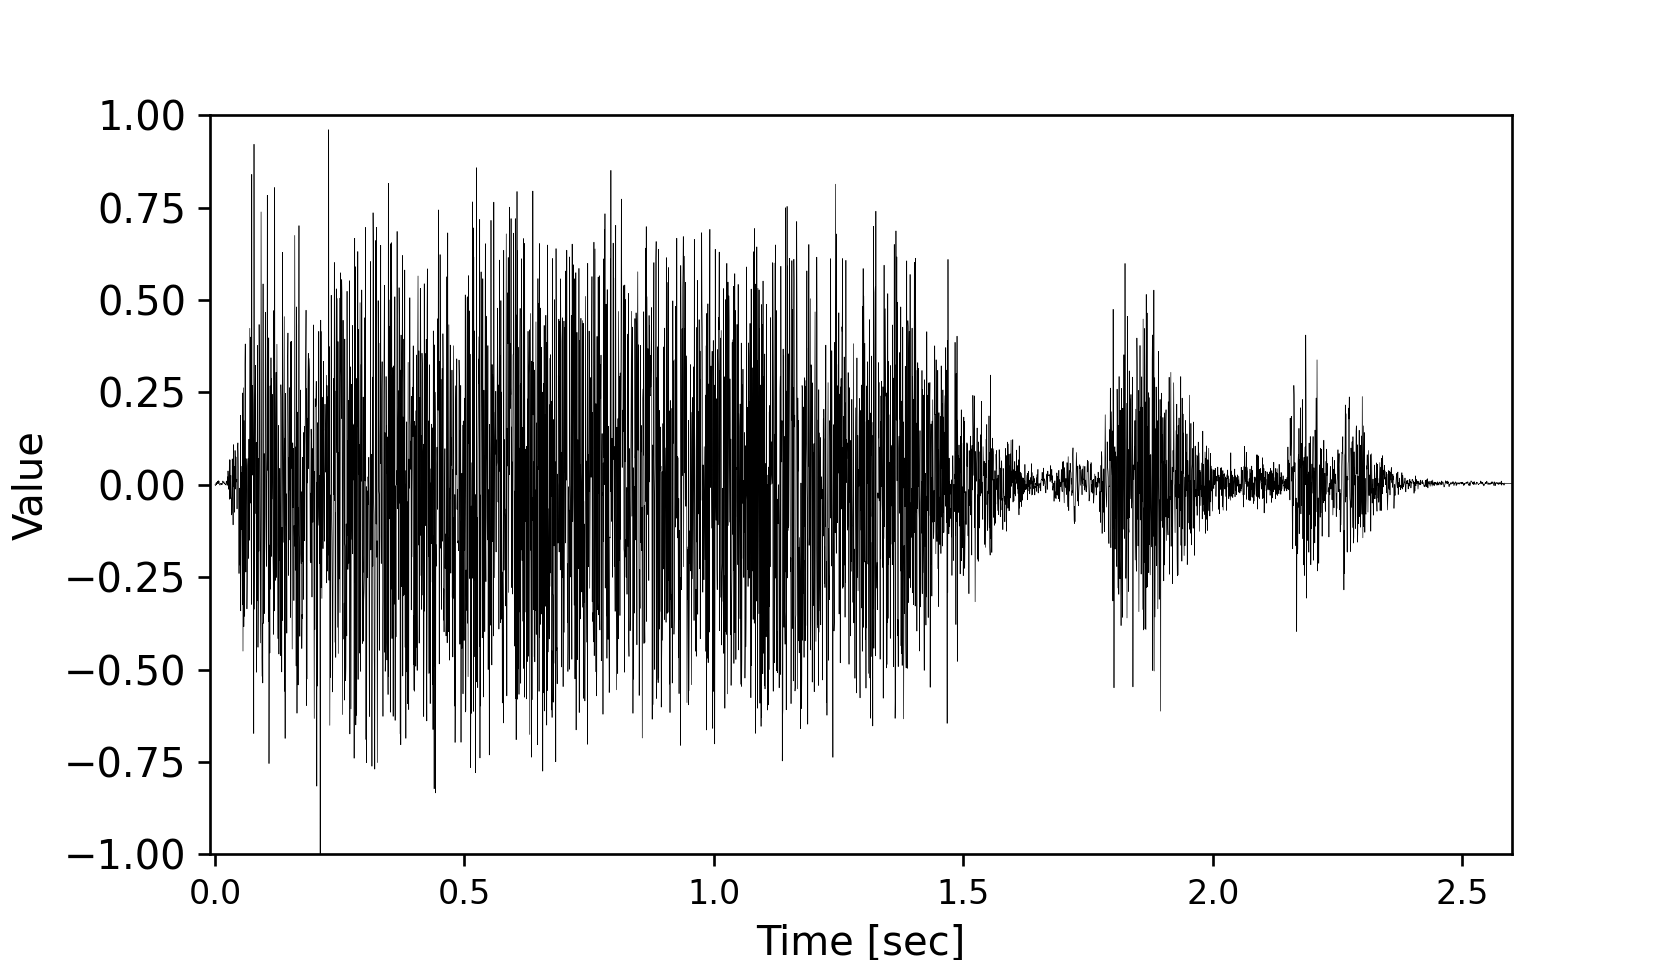
\includegraphics[width=0.49\textwidth]{images/waveform.png}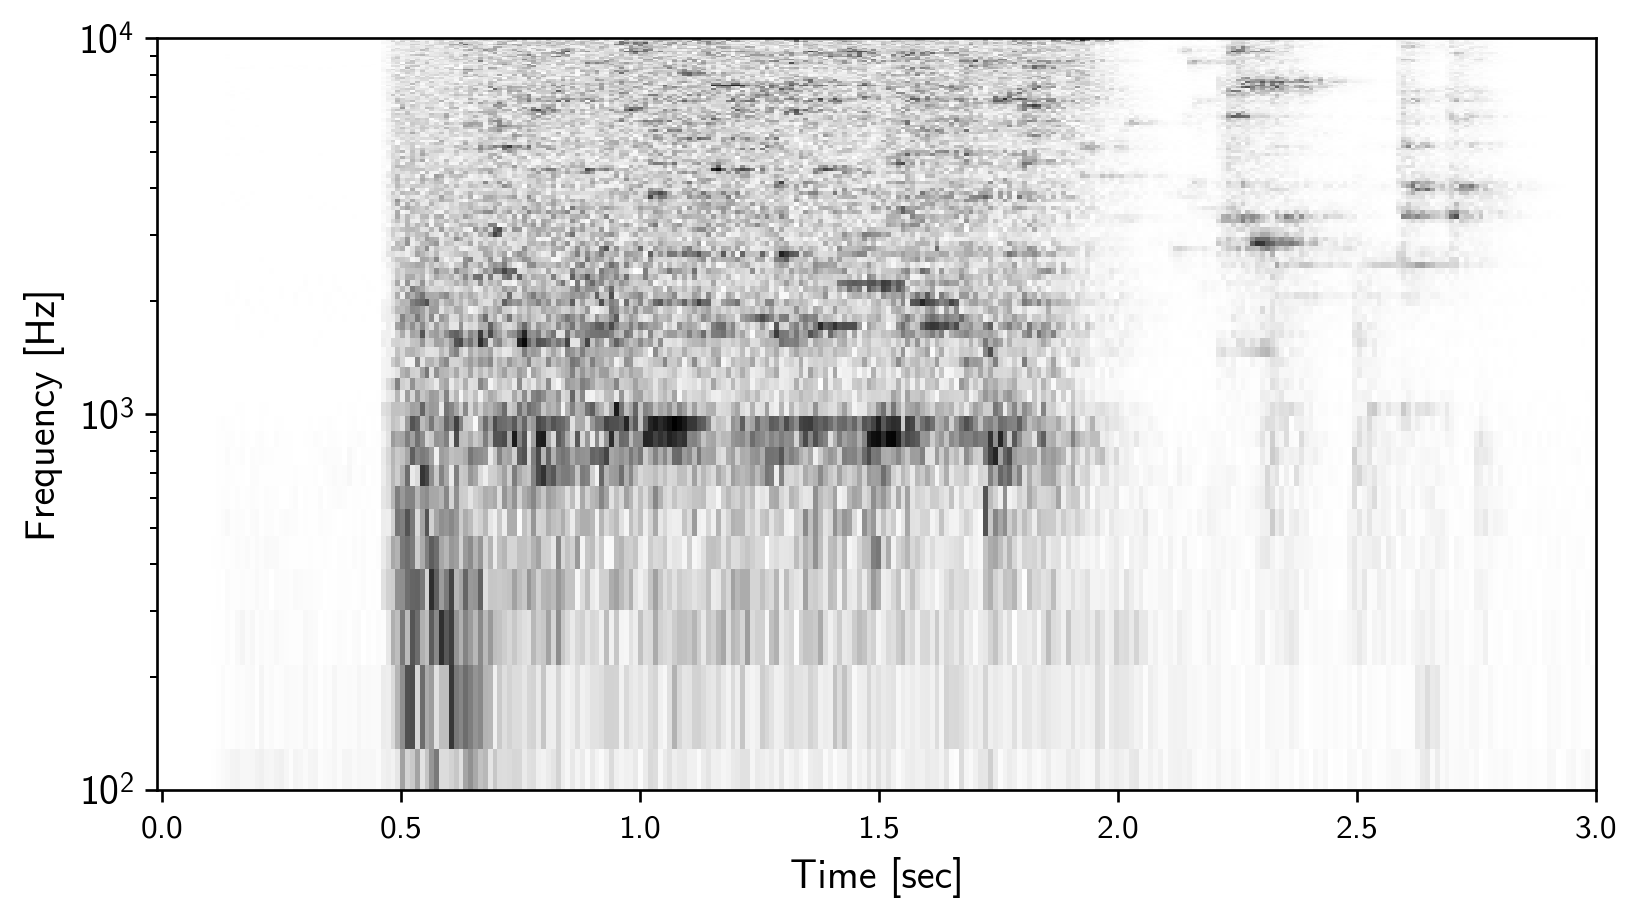
\includegraphics[width=0.49\textwidth]{images/spectrogram.png}
\caption[A comparison of two different representations of the same sound.]{A comparison of two different representations of the same sound: a glass break: \emph{waveform} (left) and \emph{spectrogram} (right). The audio is rich in various frequency bands.}
\end{figure}

The spectrogram representation is vital for retrieving frequency information, aiding in the extraction of features such as pitch (the fundamental frequency) and timbre. However, short-time Fourier transforms are constrained by a trade-off between time and frequency resolutions. Achieving high resolution in one inherently limits the resolution in the other \cite[p.~365--366]{Smith1999}.

\section{Symbolic Representation}

Symbolic representation encodes music through structured, discrete set of symbols, which abstracts certain musical elements such as pitch, duration or dynamics. The ISO/IEC 14496-23:2008 defines \emph{Symbolic Music Representation} (SMR) as \emph{a logical structure based on: symbolic elements representing audiovisual events, the relationship between those events, and aspects related to how those events can be rendered (visually as music notation or audibly) and synchronized with other media types} \cite{ISO2008}.

The definition encompasses various forms of a musical notation, with traditional sheet music as the most established form.

\subsection{Sheet Music}

\emph{Sheet music}, also known as a \emph{score}, is a form of musical notation that can be handwritten or printed. It utilizes musical symbols to represent various elements such as the pitches, rhythms, and chords of a song or an instrumental piece \cite{Wiki2024B}. Sheet music provides essential information that enables musicians to perform a piece.

There are many forms of sheet music notation, originated in different cultures. The music notation of our interest is the notation of Western Classical Music, originated in Europe.

\begin{figure}[ht!]
\centering
\includesvg[width=\textwidth]{images/prelude_gen.svg}
\caption[First bars of Frédéric Chopin's \emph{Prelude Opus 28, No. 4}.]{First bars of Frédéric Chopin's \emph{Prelude Opus 28, No. 4} \cite{Chopin1839}.}
\label{prelude_opus_28_4}
\end{figure}

Western sheet music is a symbolic representation of music that employs a set of standard notations to convey the elements of a musical composition. Key elements include:
\begin{itemize}
   \item \emph{Staff}: Consisting of five horizontal lines and four spaces, each representing a different musical pitch \cite[p.~27]{Read1969}.
   \item \emph{Clef}: Positioned at the beginning of the staff, it specifies the pitch of the notes on the staff (e.g., treble clef $\clefGInline$, bass clef $\clefFInline$ \cite[p.~51--55]{Read1969}. For instruments of a wide pitch range (such as piano), it may change during the course of a piece to accommodate the varying pitch ranges.
   \item \emph{Notes and Rests}: Symbols that represent the pitch and duration of musical sounds and silences, such as whole note $\wholeNote$, half note $\halfNote$, quarter note $\quarterNote$, etc., and corresponding rests like whole rest $\wholeNoteRest$, half rest $\halfNoteRest$, quarter rest $\crotchetRest$, etc. Dotted notes, like the dotted half note $\halfNoteDotted$, are extended by half their length, equating to three quarter notes in this example. For further information, refer to \cite[p.~64--65, 96, 103, 113--114]{Read1969}.
   \item \emph{Key Signature}: Indicates the music's key by specifying consistently altered \emph{flats} ($\flat$) or \emph{sharps} ($\sharp$) \cite[p.~135--136]{Read1969}. For example, a sharp symbol $\sharp$ next to the clef: \[\includesvg{images/key_signature_gen.svg}\] as seen in Figure \ref{prelude_opus_28_4}, signifies that each note on the indicated line should be played a semitone higher (in this case, $\textrm{F}\sharp$ instead of $\textrm{F}$), corresponding to the $\textrm{E}$ minor scale (enharmonically equivalent\footnote{Two notes are \emph{enharmonically equivalent} if they have the same pitch but are notated differently \cite[p.~10]{Kostka1994}. This is a property of the standard twelve-tone equal temperament tuning (12-ET). Other tuning systems may not have this property.} to $\textrm{G}$ major).
   \item \emph{Tempo Marking}: Indicates a song's tempo, specifying the duration of a note. This can be an exact \emph{beats per minute} (BPM) value, such as $\quarterNote = 90$, or described conventionally using Italian terms, ranging from \emph{larghissimo} (extremely slow, under 40 BPM) to \emph{prestissimo} (extremely fast, over 208 BPM) \cite[p.~276--277]{Read1969}.
   \item \emph{Time Signature}: Dictates the rhythmic structure by defining the number of beats per measure and the note value for one beat \cite[p.~148--150]{Read1969}. Represented as a fraction $\mathbf{\genfrac{}{}{0pt}{2}{n}{m}}$, with the denominator $m$ being a power of 2. For example, $\lilyTimeSignature{3}{4}$ indicates three quarter notes per measure. Common time signatures like $\lilyTimeC$ and $\lilyTimeCHalf$ are equivalent to $\lilyTimeSignature{4}{4}$ and $\lilyTimeSignature{2}{2}$, respectively.
   \item \emph{Dynamics}: Symbols and terms indicating the volume of the music, marked from $\lilyDynamics{ppp}$ (pianississimo), through $\lilyDynamics{mp}$ (mezzo piano) and $\lilyDynamics{mf}$ (mezzo forte), to $\lilyDynamics{fff}$ (fortississimo) \cite[p.~250]{Read1969}. These markings are interpretative and not absolute.
   \item \emph{Articulation Marks}: Instructions on the execution of notes, such as staccato or legato, visually represented by accents and slurs \cite[p.~260--268]{Read1969}.
\end{itemize}

A score of a music piece is comprehensive enough to encapsulate a variety of musical elements, serving as a detailed blueprint for performers to interpret and bring to life the composer's intentions. However, the sheet notation as it is cannot be used by computers directly. Thus we need to limit ourselves only to digital representations of musical scores.

\subsection{Musical Instrument Digital Interface}

The standard for music communication is \emph{Musical Instrument Digital Interface} (MIDI). However the term MIDI is overloaded and means usually several things:
\begin{itemize}
   \item A protocol enabling musical information (notes, velocities, control signals) communication between electronic devices.
   \item A technical standard detailing the specifications for digital interfaces and hardware connectors.
   \item An abstraction representing musical information encompassed within the MIDI protocol.
   \item A file format that stores a sequence of recorded MIDI messages.
   \item A MIDI stream, or a content of a MIDI file.
\end{itemize}

The specific interpretation of MIDI depends on the context. In this work, \emph{performance MIDI} refers to the last point, where the stream is captured through a digital piano or other MIDI-compatible digital keyboards\footnote{Although MIDI is not exclusively used for keyboards, the primary focus of the deep learning methods discussed here is on piano compositions.}.

A MIDI stream comprises events, each consisting of two components: a MIDI time and a MIDI message. The time value indicates the duration to wait before executing the next message in the MIDI data sequence \cite[p.~3]{Oliveira2017}. There are two principal message types:
\begin{itemize}
\item \emph{Note on}: Sent when a performer presses a key on an instrument.
\item \emph{Note off}: Triggered when a player releases a key, turning off the corresponding note.
\end{itemize}

Each message specifies two values: \emph{pitch} and \emph{velocity}\footnote{A note intensity, usually correlated with the volume, but not necessarily. This term derives from how some digital instruments measure the speed at which a key is pressed. Some instruments may not respond to this attribute at all \cite[p.~22]{Huber2007}.}. All values are encoded by a $7$-bit integer, from $0$ to $127$.

MIDI streams do not encode sound nor they specify it. The sound rendering is not a responsibility of the MIDI protocol.

The MIDI standard is built upon the 12-tone equal temperament (12-ET) system, which divides an octave into 12 logarithmically equal parts\footnote{The frequency of a note is perceived logarithmically.}. This system is represented in the conventional 88-key keyboard layout, ranging from $\textrm{A}0$ to $\textrm{C}8$, corresponding to MIDI pitch values within the range of $[21, 108]$. The relationship between frequency and pitch in standard tuning\footnote{The widely accepted standard tuning, A440, established by ISO \cite{ISO1975}, sets the frequency of the $\textrm{A}4$ note at $440$ Hz. This $\textrm{A}4$ note corresponds to the MIDI pitch value of $69$.} is expressed by the formula: \[m = 12 \log_2\left(\frac{f_m}{440\textrm{ Hz}}\right) + 69\] where $m$ is the pitch for a given frequency $f_m$ \cite[p.~47--48]{MIDI1996}.

\begin{figure}[ht!]
\centering
\resizebox{1.0\linewidth}{!}{
\begin{tikzpicture}

\coordinate (origin) at (0,0);
\coordinate (stave) at (origin);
% left line of first key
\draw (9.25,-1) -- (9.25,-5);

\def\midiC{0}
\def\midiD{2}
\def\midiE{4}
\def\midiF{5}
\def\midiG{7}
\def\midiA{9}
\def\midiB{11}

% Define a command to calculate the MIDI note number
\newcommand{\midiNote}[3]{% #1 is pitch, #2 is octave
    % Assign MIDI note numbers to each pitch (C=0, C#=1, D=2, ..., B=11)
    \pgfmathtruncatemacro{\pitchValue}{\csname midi#1\endcsname}
    \pgfmathtruncatemacro{\midiNumber}{12 + \pitchValue + #2 * 12 + #3}
};

\newcommand{\drawPianoKey}[4]{
	\pgfmathparse{#2*7+\p+0.25-#3}
        \edef\myx{\pgfmathresult}
        % draw three lines for top, right, bottom of this key
        \draw (\myx,-1) -- (\myx,-5);
        \draw (\myx,-1) -- ($(\myx,-1)+(-1,0)$);
        \draw (\myx,-5) -- ($(\myx,-5)+(-1,0)$);
        % print pitch on line
        \node [anchor=base,xshift=-15] at (\pgfmathresult,-4.5) {{#1}{#2}};
        
		\midiNote{#1}{#2}{0};
    		\node[anchor=base,xshift=-15] at (\pgfmathresult, -5.5) {\midiNumber};

        \blacknotefalse
        \ifcase\p
        \or
            \blacknotetrue
        \or
          \ifnum#2>0
            \blacknotetrue
          \fi
        \or
        \or
            \blacknotetrue
        \or
            \blacknotetrue
        \or
            \blacknotetrue
        \else
        \fi
        \ifblacknote
            % recalculate x
            \pgfmathparse{#2*7+\p-#3}
                \fill ([xshift=0.25cm, yshift=-1cm]stave.south -| \pgfmathresult,0) ++(-0.25cm,0) rectangle ++(0.5cm,-2.5cm);
                % print pitch on black key
                \node [anchor=base,xshift=0.25cm,white] at (\pgfmathresult,-2.5) {\textbf{#1}$\sharp$};
		        \midiNote{#1}{#2}{1};
    		       \node[anchor=base,xshift=0.25cm] at (\pgfmathresult, -0.75) {\midiNumber};
        \fi
}

\newif\ifblacknote
\foreach \octave in {2,...,5}
    \foreach \pitch [count=\p] in {C,D,E,F,G,A,B}{
        % calculate x position from octave and pitch
        \drawPianoKey{\pitch}{\octave}{5}{15}
    }

\def\p{7}
\drawPianoKey{C}{6}{11}{21}
\end{tikzpicture} 

}
\caption[A piano keyboard layout with 49 keys.]{A piano keyboard layout with 49 keys. The integers stand for MIDI note values.}
\end{figure}

A velocity value for a played note should be non-zero, typically controlling the volume of the note. However, there is no universal agreement on the exact gain corresponding to a given velocity value.

The smallest MIDI time unit is \emph{tick}. The length of a single tick is determined by two MIDI parameters:
\begin{enumerate}
	\item \emph{tempo}, which describes microseconds per quarter note.
	\item \emph{ticks-per-quarter-note}, with a common value of $480$.
\end{enumerate}

For example, in the tempo of 120 beats per minute (BPM) the quarter note lasts 500,000 microseconds. In that case, assuming 480 ticks per quarter note, one tick lasts: \[\textrm{tick length} = \frac{\text{ 500,000 microseconds}}{\text{480 ticks}} = 1041.67 \text{ microseconds}\] This feature allows MIDI to handle both physical lengths, as well as musical ones.

While this work primarily focuses on MIDI representation, other notable symbolic representations include:
\begin{itemize}
   \item \emph{MusicXML}: An XML-based file format for representing Western musical notation, designed for both human and machine readability \cite{Good2001}.
   \item \emph{ABC}: A simplified musical notation system encoding essential musical elements \cite{ABC2013}.
   \item \emph{LilyPond}: As authors claim, \emph{LilyPond} is \emph{designed to solve the problems we found in existing software and to create beautiful music that mimics the finest hand-engraved scores} \cite{LilyPond2002}. \emph{LilyPond} has been used to generate all scores and musical glyphs present in this dissertation.
\end{itemize}

Symbolic notation has its limitations: it can only describe predefined musical aspects, ignoring a multitude of other factors\footnote{This is, as any kind of abstraction, rather a desired property.}. For instance, the sheet notation does not capture the timbre of sound and is very limited in expressing dynamic sound ranges. While the format was not primarily designed to represent symbolic music but to allow communication between musical devices, it may be used for that purpose as it can handle musical as well as physical onset times and note durations \cite{Grohganz2014}.

Most symbolic representations are based on the standard division of an octave into 12 tones, which makes them less suitable for music from non-Western European traditions, such as the Indonesian pentatonic \emph{slendro} or seven-note \emph{pelog} systems, for gamelan instruments \cite[p.~73]{Sethares2005}. Certain music genres, like \emph{musique concrète}, are not expressible through traditional notation at all \cite[p.~69--77]{Schaeffer2012}.

In the context of this work, we limit ourselves to the heritage of Western European Music, as we are focused on classical European piano works, composed by Bach, Mozart, Beethoven, Schubert, Chopin, Liszt and others.


\chapter{Automatic Music Transcription}

\emph{Automatic Music Transcription} (AMT) is the design of computational algorithm converting an acoustic musical signal into some form of musical notation, such as sheet music or MIDI files \cite{Benetos2019}. AMT is a subset of the broader field of \emph{Music Information Retrieval}.

\section{Music Information Retrieval}

\emph{Music Information Retrieval} (MIR) is an interdisciplinary research field concerning extraction and inference of meaningful features from music, indexing of music using these features, and the development of different search and retrieval schemes \cite{Schedl2014}.

It involves several different scientific backgrounds such as: musicology, psychoacoustics, signal processing, informatics, and most recently, machine learning \cite{Wiki2024A}.

The acronym MIR (\emph{Musical Information Retrieval} was first used by Kassler in 1966, referring to a special-purpose programming language named MIR \cite{Kassler1966}. However, the term has significantly evolved since then.

\subsection{Examples of Problems in Music Information Retrieval}

The scope of Music Information Retrieval is very extensive. It includes but is not limited to:
\begin{itemize}
	\item \emph{Classification and Indexing}. The amount of available digital music is constantly increasing \cite{Orio2006} and there is a need to organize music data into categories in order to facilitate navigation through rich audio libraries, link related audio items or managing music archives.
	\item \emph{Audio Identification}. This task aims to identify a fragment of a given music recording under conditions of recording noise or other distortions. A well-known system for this purpose is \emph{Shazam}. A variant of this task is \emph{query by humming}, where a user hums or sings a melody, and the system recognizes the corresponding song \cite{Schedl2014}.
	\item \emph{Measuring Music Similarity}. This involves comparing different music pieces to determine their similarity. Analysis may include melody, harmony, rhythm, and lyrics, aiding in genre classification, mood-based recommendations, and identifying cover songs or similar musical styles \cite{Berenzweig2003}.
	\item \emph{Instrument/vocal recognition and separation}. The most general expression of the problem is to identify and separate each instrument from a given audio sample. A specific application is separating a vocal track from a full song.
	\item \emph{Recommendation Systems}. Certain music systems propose a list of music pieces (usually \emph{playlists}) based on user musical preferences with some parameters involved: \emph{accuracy}, \emph{diversity} or \emph{serendipity} (a measure how surprising a recommendation is) \cite{Schedl2014}.
	\item \emph{Audio Transcription}. In this task, audio recordings are converted into a written or symbolic form, such as sheet music or MIDI files. This involves detecting and notating various elements like pitches, rhythms, and possibly lyrics from the audio signal.
\end{itemize}

Our primary interest lies in the last area, audio transcription, which will be the focus of the next section.

\subsection{Sources of Music Information}

While the general scope of tasks and problem in Music Information Retrieval is very broad, the information can primarily be sourced from two categories of music representation: \emph{audio-based} and \emph{symbolic}. These two primary modes of representing music information have been discussed in detail in the preceding chapter.

Besides the two previously mentioned ways of music representation, there is also a bibliographic source of information. That includes: title, composer/arranger/performer, publisher, publication date, and sometimes additional information such as the date of a recording, information about the label publishing, catalog numbers, or music categorization by genre or style. Such bibliographic details can be integral to certain MIR systems, offering a different dimension of information beyond the audio and symbolic representations.

\subsection{Music Facets}

There are many aspects of musics one wish to extract from. Downie lists a few aspects, though not mutually exclusive, that can be subject to Music Information Retrieval \cite{Downie2003}:
\begin{itemize}
	\item \emph{Pitch Facet}.
	\item \emph{Temporal Facet}.
	\item \emph{Harmonic Facet}.
	\item \emph{Timbral Facet}.
	\item \emph{Editorial Facet}.
	\item \emph{Bibliographic Facet}.
\end{itemize}

Extracting each of these facets involves distinct methodologies as they operate on different layers of musical information.

For instance, generating a complete score from a performance MIDI requires the extraction of pitch, temporal, and editorial facets. While pitch and temporal aspects are present in the MIDI stream, the underlying harmonic and temporal structures, such as key and time signature, are not explicitly present and must be inferred.

In case of pitch, even for a MIDI file, ambiguity is still possible. For example, a MIDI note represented by the number 73 could, depending on the musical context, be interpreted as either $\textrm{C}\sharp$ or its enharmonic equivalent, $\textrm{D}\flat$. Similarly, note lengths are usually not preserved. For instance, a pianist's hand movement between notes (unless playing \emph{legato}) typically shortens the actual length of a note compared to its notated duration in the score.

The list above mentioned by Downie is not exhaustive: music is a very multimodal phenomenon and it comes not only with an audio, but also text (lyrics), images (album covers and photographs of musicians) or gestures of performers \cite{Schedl2014}.

\section{Automatic Music Transcription}

As defined by Benetos et al. \cite{Benetos2019}, \emph{Automatic Music Transcription} (AMT) is \emph{the design of computational algorithms to convert acoustic music signals into some form of music notation}. Typically, the input of an AMT system is a raw audio signal, encoded in one of common audio format, whether lossless (like WAVE, AIFF, FLAC) or compressed (such as MP3, AAC, or Ogg). The output of AMT systems varies and depends on specific use cases.

Regardless of the final output form, the general AMT task is a multi-staged process involving several different subtasks:
\begin{enumerate}
	\item Instrument recognition and separation
	\item (Multi-)pitch estimation
	\item Note onset and offset detection
	\item Beat and rhythm tracking
	\item Interpretation of dynamics
	\item Interpretation of instrument articulations
	\item Score typesetting
\end{enumerate}

AMT systems may focus on addressing only a subset of these problems, meaning not all stages are necessarily involved in every AMT task. Therefore, AMT should be viewed not as a singular task but as a class of various tasks. Often, the audio sample may be pre-processed into an intermediate form, such as a MIDI stream, before being subjected to further AMT processing.

\subsection{Application of Music Transcription}

AMT systems can be applied to facilitate a variety of routine tasks that musicians would do manually otherwise.

Benetos et al. (2013) highlights that one of \emph{the most immediate application of automatic music transcription is for allowing musicians to record the notes of an improvised performance in order to be able to reproduce it} \cite{Benetos2013}.

These systems can significantly aid in the learning process for individuals wishing to practice songs for which published scores are either unavailable or hard to access. These systems also may speed up the process of composing, when the tedious task of transcribing recordings is no longer necessary. The latter is the promise of performance MIDI to score transcription systems.

\subsection{Levels of Music Transcription}

Music transcription can be classified into four distinct levels: \emph{frame-level}, \emph{note-level}, \emph{stream-level}, and \emph{notation-level}, each with its unique purposes and challenges \cite{Benetos2019}.

\subsubsection{Frame-level Transcription}

\emph{Frame-level transcription}, also known as \emph{multi-pitch estimation} (MPE), involves estimating the pitch of notes at the level of individual samples (or frames), treated independently for each frame \cite{Bhattarai2023}. This form of transcription may be conducted under the assumption of either monophonic or polyphonic instrumentation, with the latter being more complex.

The outcome is a partial function (or a set of such functions) $f\colon I\to\mathbb{R}_{>0}$ where for each point of time $x\in I$ a frequency is assigned. Additionally, frame-level transcription often includes sound energy estimation.

This level of transcription is vital for pitch-correction tools such as \emph{Melodyne}. However, this level of transcription fails to capture a broader context of music structure.

\subsubsection{Note-level Transcription}

\emph{Note-level transcription} is one abstraction layer higher than frame-level transcription. It aims to estimate an entire note entity, recognize a note's pitch within a note onsets and offset. It often includes determining note velocities.

One possible format of the output of note-level transcription is a MIDI stream.

\begin{figure}[ht!]
\centering
\begin{tabular}{>{\centering\arraybackslash} m{0.05\textwidth} >{\centering\arraybackslash} m{0.95\textwidth}}
1 & \includesvg[width=0.9\textwidth]{images/pitch_estimation.svg}\\
2 & \includesvg[width=0.9\textwidth]{images/pitch_notes.svg}
\end{tabular}
\caption[A frame-level and note-level transcription of a vocal audio sample.]{A frame-level (1) and note-level (2) transcription of a vocal audio sample. The \emph{CREPE} algorithm has been used for a monophonic pitch estimation \cite{Kim2018}, and \emph{CREPE notes} for note quantization \cite{Riley2023}. Frequency instability leads to misaligned pitch attribution on a note-level transcription.}
\end{figure}

\subsubsection{Stream-level Transcription}

\emph{Stream-level transcription}, also known as \emph{multi-pitch streaming} (MPS), involves grouping estimated pitches or notes into separate streams, typically corresponding to individual instruments \cite{Bhattarai2023}. On that level of transcription, multi-pitch estimation is not sufficient as distinguishing different instruments is needed. The process of instrument differentiation is in fact a clustering problem.

Instruments differ in their timbres, or tone colors, which is the perceived quality of sound that makes two instruments sound distinct even when they play the same pitch at the same energy level. The timbre largely depends on an instrument's harmonic series and its variation over time (the envelope). This is merely a simplification: not all sounds conform to harmonic series representations; for example, noise or most percussion instruments are exceptions, though tonal instruments are generally well-described by harmonic series \cite[p.~27--28]{Sethares2005}.

Duan et al. (2014) defines the streaming tasks as: \emph{the clustering objective is to maintain timbre consistency, based on the assumption that sound objects coming from the same source have similar timbre} \cite{Duan2014}. Notes coming from the same instrument are expected to have similar timbre characteristic. Depending on the method, the number of instrument clusters may or may not be specified beforehand.

The timbre of an instrument is not static and can vary based on several factors, including:
\begin{itemize}
	\item The method and force of inducing vibration. For instance, a violin emits different sounds based on the bowing technique, and a piano's sound quality changes with the force applied to the keys.
	\item The fundamental frequency. The harmonic series of an instrument varies with the played note, often resulting in different overtone distributions in lower and higher registers.
	\item Playing technique. The way a musician produces sound can significantly affect timbre. On wind instruments, for example, variations in embouchure, tonguing, and breath control can create diverse timbral effects.
\end{itemize}

The timbre clustering becomes particularly challenging when similar but distinct instrument are played simultaneously, and their harmonic series are overlapping.

\subsubsection{Notation-level Transcription}

\emph{Notation-level transcription} is the process of converting audio recordings into a traditional music notation or a score \cite{Bhattarai2023}. This process transforms the musical content into a structured format as outlined in the previous section on \emph{Sheet Music}.

Besides the musical content, that is notes and rests, notation-level transcription involves assigning other various musical elements:
\begin{itemize}
	\item Instruments are organized by separate staves. Each instrument needs to be recognized and appropriately organized within the score.
	\item Tempo markings are usually indicated at the beginning of a piece but may vary throughout the composition.
	\item Clefs are used to suggest the pitch range of the voice or instrument. For instruments with a wide pitch range, such as the piano, the clef may change during the piece.
	\item Time signatures are essential, with the most common default being $\lilyTimeSignature{4}{4}$. While the time signature generally remains consistent across instruments, it can vary within a piece.
\end{itemize}

Some notation-level transcription methods might come with certain limitations and not provide all these elements. For instance, they might default to using the $\textrm{C}$ major treble clef and the common $\lilyTimeSignature{4}{4}$ time signature for all staves, regardless of the song's actual key or time signature. Some methods may also assume that a single instrument is being played.

\subsection{Stages of Music Transcriptions}

As previously discussed, the general transcription is a complex task consisted of several steps.

Assume we have a raw audio signal containing a recording of music. For the sake of simplicity, let us consider a raw audio signal containing a recording of music from a single polyphonic instrument such as piano or guitar.

In order to retrieve notes from the recording, usually the audio signal is converted to a spectrogram. This representation allows both pitch and energy estimation.

The transcription involves three challenges:
\begin{itemize}
	\item \emph{Detecting Pitch Frequencies}. Notes usually produce a series of harmonics – multiples of a fundamental frequency – each with varying energy levels that change over time. Additionally, the fundamental frequency itself may fluctuate due to vibration and glide. This task is further complicated by the limited frequency resolution of the short-time Fourier transform.
	\item \emph{Recognizing Time Onsets and Offsets}: Identifying when a note begins and ends is straightforward in monophonic music but becomes significantly more complex in polyphony, where multiple notes are often played with slightly different timings, and their envelopes overlap with each other. As in the previous task, time resolution of the short-time Fourier transform is limited as well.
	\item \emph{Measuring Note Velocity}. Notes can be played with different energy, resulting a sound with different amplitude. Accurately assigning velocity to each note is difficult, especially when notes have overlapping harmonic series and energy attribution becomes ambiguous. Also a limited resolution of a Fourier transform contribute to this effect.
\end{itemize}

There are different strategies to overcome these obstacles. Assuming that there is only one instrument playing, these are covered by note-level transcription.

The outcome of this process is a \emph{performance MIDI} or a \emph{MIDI stream}, comprising a sequence of notes characterized by four features: pitch, note onset, duration, and velocity.

A MIDI stream lacks information about the underlying music structure. More specifically, certain vital score elements are still yet to be determined: time signatures, key signatures, voicing (e.g. hand part assigning for piano recordings). Moreover, notes and rests need to be quantized into standardized lengths (e.g., whole notes $\wholeNote$, half notes $\halfNote$, quarter notes $\quarterNote$, etc.).

The final stage is notation-level transcription: transforming the performance MIDI into a scored format. This involves imposing the structure mentioned above and then rendering the score in a specific music data format.

\begin{figure}[ht!]
\centering
\begin{tabular}{>{\centering\arraybackslash} m{0.05\textwidth} >{\centering\arraybackslash} m{0.95\textwidth}}
1 &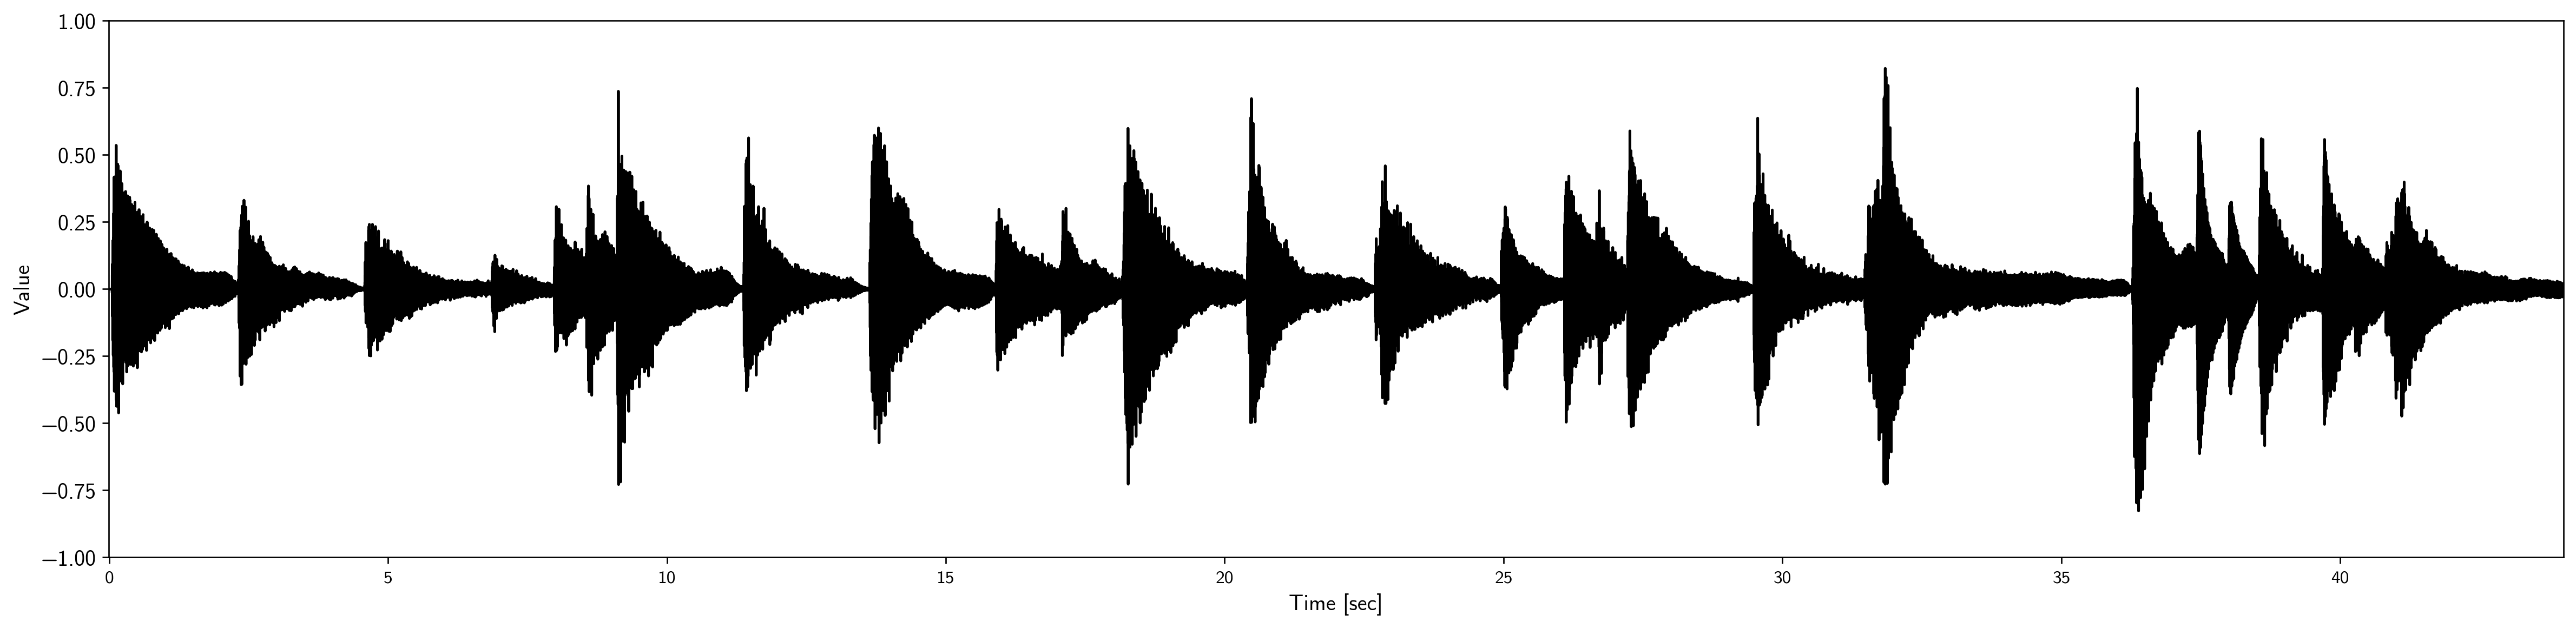
\includegraphics[width=0.9\textwidth]{images/amt_0.png} \\
2 &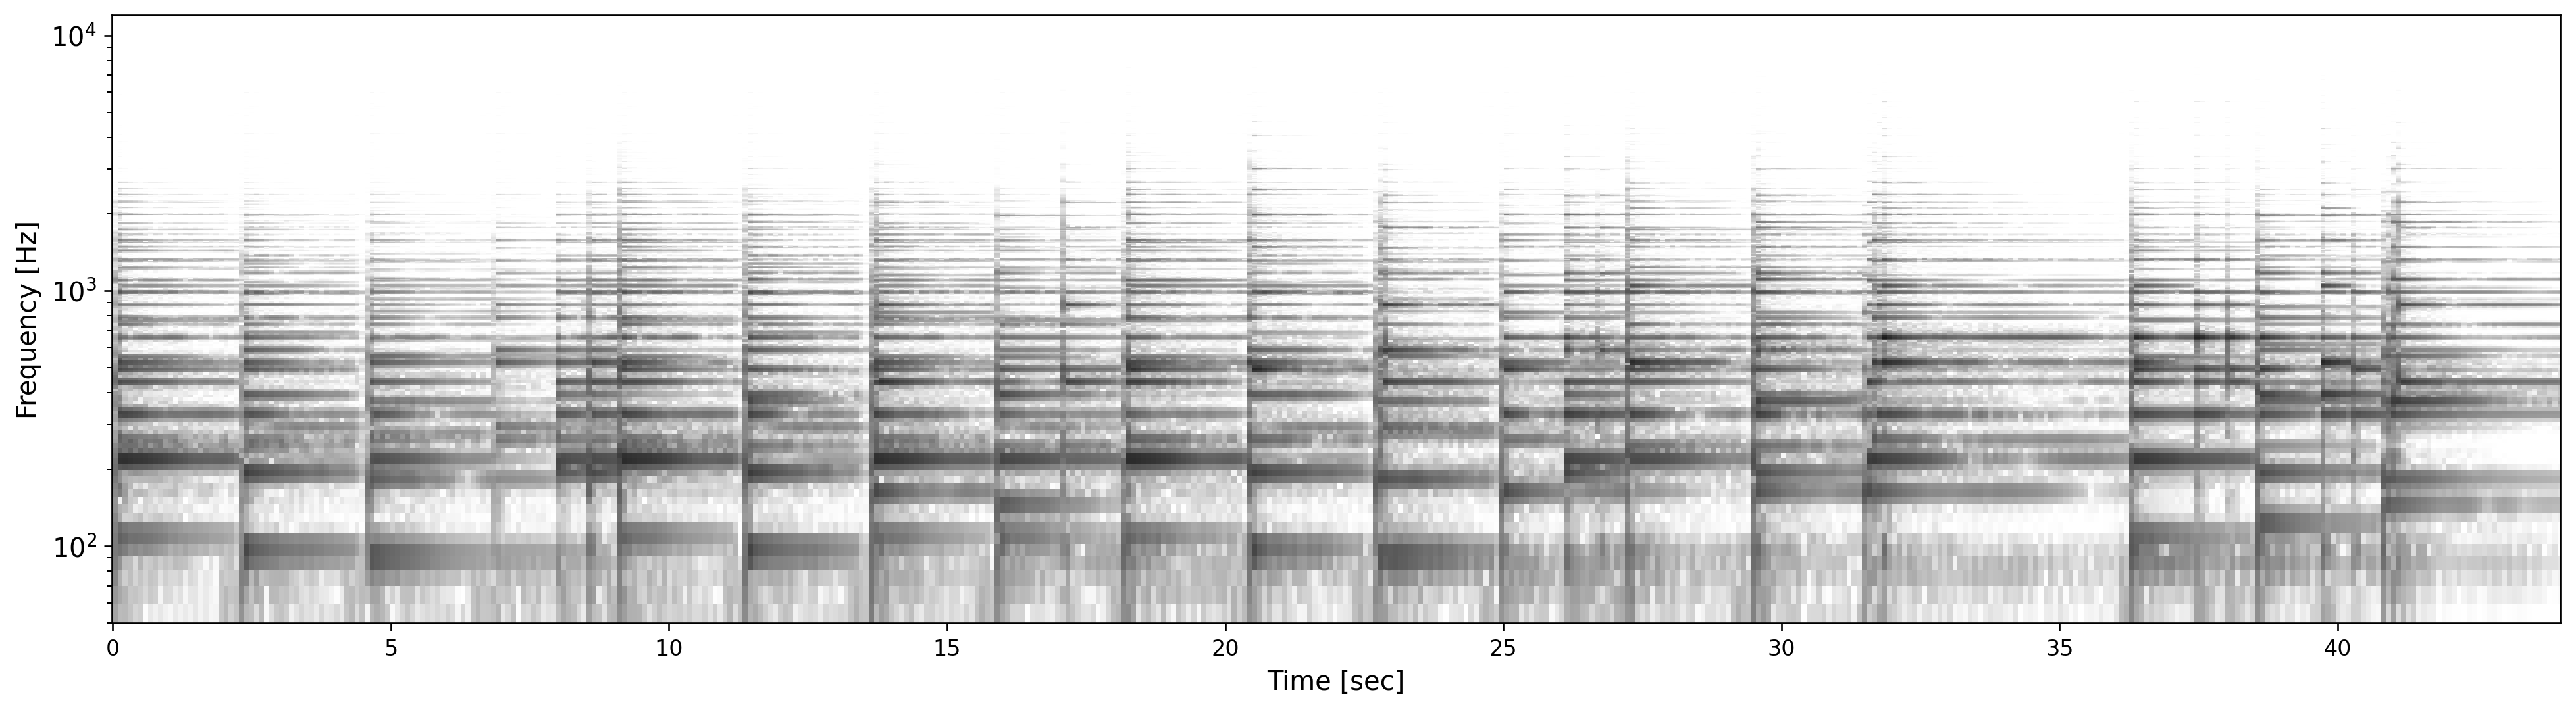
\includegraphics[width=0.9\textwidth]{images/amt_1.png} \\
3 &\includesvg[width=0.9\textwidth]{images/piano_roll.svg} \\
4 &\includesvg[width=0.9\textwidth]{images/amt_gen.svg}
\end{tabular}
\caption[An example of an Automatic Music Transcription task on a concrete piano recording.]{An example of an Automatic Music Transcription task on a concrete piano recording. First, the audio sample (1) is transformed to a spectrogram (2) using the short-time Fourier transform, from which notes are retrieved. The result of that process is a sequence of a MIDI stream (3) for which the other aspects of music score are determined (here: clefs, key signature, time signature, tempo marking) and transcribed to a final score (4).}
\end{figure}

This stage of audio transcription is the main focus of this work, concerning mostly on digital piano recordings. From now on we will assume that the performance MIDI is given, either retrieved from the audio signal, or recorded directly via some MIDI instrument. However, we do not care about the visual aspects of the score, only its content. The more precise definition of \emph{content} will be formalized in the next fragment.

\subsection{Performance MIDI to Score Transcription}

Let us review basic assumptions of the performance MIDI to score process. In this section, we follow the name convention of Liu et al. (2022), the authors of the main performance MIDI to score model discussed \cite{Liu2022}. However, a few adjustments have been made.

\subsubsection{Performance MIDI Encoding}

The input performance MIDI may be encoded as a sequence $\mathbf{X}=\left\{p_i,o_i,d_i,v_i\right\}_{i=1}^N$ of a variable length $N$, of four features: \emph{pitch} $p_i$ (an integer from the range $0$ to $127$), \emph{onset} $o_i$ being a positive real number, \emph{duration} $d_i$, also a positive real number, and \emph{velocity} $v_i$, an integer from range $0$ to $127$. The velocity may be further normalized to a rational number from the unit interval. We assume also that the sequence is sorted firstly by the onset, and secondly by the pitch in the ascending order.

The encoding of a performance MIDI is in fact a two-dimensional tensor. We will call such encoding also a performance MIDI, when no confusion arises.

\subsubsection{Music Score Encoding} \label{music_score_encoding}

In this section, we define a music score in terms of the essential elements it needs to encode. The output of our automatic transcription method focuses solely on the abstract elements of a score, entirely disregarding the visual layout.

These elements include:
\begin{itemize}
	\item \emph{Tempo}, quantized as an integer within the range of $0$ to $200$. Practically, only values above $30$ are  expected.
	\item \emph{Downbeats} and \emph{beats}, marking sections of each measure\footnote{The downbeat is the first beat of a measure.}. This segmentation helps convert a rhythmically unstructured MIDI into structured measures and identify the initial beats of these measures. Both elements are binary.
	\item \emph{Musical onsets}, indicating the start of notes in terms of quantized beat divisions. Whole integers correspond to notes beginning on a downbeat.
	\item \emph{Note values}, representing durations as quantized lengths (e.g., $1$ for a whole note, $\frac{1}{2}$ for a half note). However, note values are categorical.
	\item \emph{Key signature}, chosen from one of $12$ possible scales: $\textrm{C}$, $\textrm{C}\sharp$, $\textrm{D}$, \ldots, $\textrm{A}\sharp$, $\textrm{B}$, each treated as a separate category.
	\item \emph{Time signature}, consisting of a numerator and denominator. Since there are only several common time signatures, one can narrow down the choice of possible values: $0$, $2$, $3$, $4$ and $6$ for the numerator, and $0$, $2$, $4$ and $8$ for the denominator. The value $0$ stands for other values.
\end{itemize}

Musical onsets, note values, and even key/time signatures may be assigned for each note. Beats and event downbeats may not come without notes and their prediction cannot be done on the note level.

Since we expect only piano recordings, we also aim to differentiate between left and right hand parts, represented as two staves with treble and bass clefs, respectively. This assignment is binary.

Note that pitch values are derived directly from the input. Articulation and dynamic markings are not considered within the scope of the model proposed by Liu et al. (2022).

To summarize, the output score $\mathbf{Y}$ can be represented as a pair of two tensors $\left(\mathbf{Y}_b, \mathbf{Y}_n\right)$:
\begin{itemize}
	\item The beat tensor $\mathbf{Y}_b = \left\{t_j, db_j\right\}_{j=1}^B$ encapsulates the real times $t_i$ of beats, along with a binary downbeat classification $db_i$.
	\item The note-level tensor $\mathbf{Y}_n=\left\{mo_i, nv_i, h_i, tn_i, td_i, k_i, tem_i\right\}_{i=1}^N$ where $mo_i$ is quantized music onset, $nv_i$ is the note value, $h_i$ indicates the hand part of a note (left or right), $tn_i$ and $td_i$ are time signature numerators and denominators, $k_i$ is the key signature, and $tem_i$ is the BPM represented as an integer. All values are categorical.
\end{itemize}

The objective of performance MIDI to score automatic transcription is to find a good enough function $\mathbf{X}\to\mathbf{Y}$. Further sections will be devoted to measuring the quality of the resulting score in order to define the \emph{good enough} part. 

\section{Challenges in the Transcription Task}

Before providing an overview of methods for MIDI to score conversion, it is essential to first understand the inherent challenges of the transcription task. We need to examine how a performance captured in a MIDI file deviates from traditional sheet music and identify the types of information that are lost in the process of translating between these two forms of musical representation.

Some challenges are directly related to the way musical data is encoded in the MIDI format, such as the issue of \emph{note spelling}\footnote{See the Section \ref{harmonic_equivalence} for the explanation.}. This leads to ambiguities that require further disambiguation through additional algorithms or human intervention.

Other challenges arise from the nature of musical performance itself and the variations that occur when a piece is interpreted and played. A live performance rarely, if ever, adheres strictly to the abstract representations of rhythm and timing found in traditional notation. Some vital aspects of the human performance are described in more detail in the next section.

\subsection{Common Transcription Problems}

Traditional music notation represents an idealized version of how a piece should be played. While it provides a structured framework for pitch, rhythm, dynamics, and articulation, it abstracts away from many performance nuances that are either too subtle, too variable or simply irrelevant to be captured in symbolic notation.

\begin{figure}[ht!]
\centering
\begin{tabular}{cc}a)
\includesvg[width=0.3\textwidth]{images/sonata_original_gen.svg}
 & b)\includesvg[width=0.6\textwidth]{images/sonata_performance_gen.svg}
\end{tabular}
\caption[An example of the imported performance MIDI of Chopin's \emph{Sonata No. 2, Op. 35, 2nd movement} ,,as it is''.]{An example of the imported performance MIDI of Chopin's \emph{Sonata No. 2, Op. 35, 2nd movement} ,,as it is'': a) the original sheet, b) the imported performance MIDI without time/key signature assignment. Not only the actual durations render the sheet unreadable and impractical, but also introduce error resulting from note quantization. Notice that there is no hand separation.}
\label{chopin_sonata}
\end{figure}

These deviations can make the direct conversion of performance MIDI into readable sheet music difficult, as exemplified in Figure \ref{chopin_sonata}. Below, we will explore some of the most common transcription problems.

\subsubsection{Tempo}

MIDI files operate with a fixed tempo, or more precisely, a discrete set of tempo changes. A human performer, however, never aligns to the tempo perfectly, even in a course of a single measure.

In many cases, these deviations are deliberate. For example, a performer might slow down (\emph{rubato}) or sustain a note longer than notated (\emph{fermata}) for expressive purposes. While these nuances may sometimes be annotated in the score, it is not always the case, and even when marked, the precise nature of the tempo fluctuation is left to the performer’s interpretation. Performers have considerable freedom in determining the extent and suddenness of tempo changes, which MIDI struggles to represent accurately.

More importantly, performance MIDI files often do not reflect internal tempo structures, rendering the ticks-per-quarter-note parameter ineffective. This issue is further addressed in Section \ref{score-informed_midi_files}.

\subsubsection{Note duration}

In live performances, note durations often deviate from those specified in the score. Pianists, for example, tend to slightly shorten note lengths to prepare for the next note or chord.

In \emph{legato} playing, some notes may be overlapping and their actual length is a bit longer than indicated by the notation. This elongation is especially prominent in rapid, fluid passages. Conversely, \emph{staccato} notes, which are played with almost immediate release, are never denoted with actual expected time of playing. Traditional notation primarily indicates note boundaries, leaving the actual performed lengths to be interpreted by the pianist.

\subsubsection{Dynamics}

The traditional notation system offers a relatively limited palette of dynamic markings, ranging from \emph{pianississimo} ($\lilyDynamics{ppp}$) to \emph{fortississimo} ($\lilyDynamics{fff}$). Changes in volume over a phrase are marked by \emph{crescendo} ($\crescHairpin$) and \emph{diminuendo} ($\decrescHairpin$) symbols. Thorough centuries, the notation has been expanded and introduced new markings such as \emph{sforzando} (sfz) or \emph{subito forte} (sf).

The dynamics are not absolute, rather contextual and depending on the surrounding musical elements. Since these markings are guidelines, there is some room for interpretation by the performer.
	 	 
In contrast, MIDI format stores a concrete note velocity with 7-bit precision. As a rule of thumb, the following arbitrary classification is adopted:

\begin{table}[!ht]
\centering
\begin{tabular}{ccc}
    Dynamic              & Marking              & Velocity \\\hline
    \emph{pianississimo} & $\lilyDynamics{ppp}$ & 16       \\
    \emph{pianissimo}    & $\lilyDynamics{pp}$  & 33       \\
    \emph{piano}         & $\lilyDynamics{p}$   & 49       \\
    \emph{mezzo-piano}   & $\lilyDynamics{mp}$  & 64       \\
    \emph{mezzo-forte}   & $\lilyDynamics{mf}$  & 80       \\
    \emph{forte}         & $\lilyDynamics{f}$   & 96       \\
    \emph{fortissimo}    & $\lilyDynamics{ff}$  & 112      \\
    \emph{fortississimo} & $\lilyDynamics{fff}$ & 127
\end{tabular}

\caption[The dynamics table.]{The dynamics table.\missing}
\end{table}

While the MIDI format represents the dynamics numerically instead of symbolically, there is no direct translation of the actual note velocity to dynamics markings: these describe broader phrases rather than individual notes. An analysis is required to translate raw velocity data into meaningful dynamics guidelines.
	 
The standard transcription model does not handle dynamics explicitly. Experimental methods addressing this issue are discussed in Chapter \ref{experiments_and_improvements}.

\subsubsection{Harmonic Equivalence}\label{harmonic_equivalence}

As the MIDI file format does not distinguish enharmonically  equivalent pitches, we generally cannot solve the problem  of pitch spelling, that is assigning correct \emph{accidentals}: flats ($\flat$) or sharps ($\sharp$) \cite{Cambouropoulos2000}. For example, in keys like D major or G major, a MIDI note 66 is likely to be spelled as F$\sharp$, while the same pitch may function as G$\flat$ in keys such as E$\flat$ or B$\flat$ minor.

The ambiguity can be resolved through assigning the key signature, that is determining the key of the scale. This approach has been successfully used in \cite{Liu2022}.

\subsubsection{Voicing}

A \emph{voice} (or \emph{stream}) is defined as "a monophonic sequence of successive, non-overlapping musical tones" \cite{Karydis2007}. This notion can be broadened to any sequence of notes, whether monophonic or polyphonic, that is perceived as a single musical entity \cite{Cambouropoulos2008}.

\begin{figure}[ht!]
\centering
\includesvg{images/bach_fugue_gen.svg}
\caption[Four independent voices in the Fugue No.1 in C Major, BWV846 by J.S. Bach.]{Four independent voices in the Fugue No.1 in C Major, BWV846 by J.S. Bach.}
\end{figure}

A single MIDI track can be viewed as a collection of notes, and the MIDI format does not offer any levels of further subdivisions. Consequently, exporting a score to a MIDI file loses all information regarding the original voicing. For that reason in the case of piano music, it is common (but not guaranteed) to separate left-hand and right-hand notes into two tracks, corresponding to the two hands. Since there can be more voices than only indicated by the left and hand right (as the example above shows), the hand separation is a subset of a broader challenge of voice separation. For a related work in that matter, refer to \cite{Karydis2007}.
	
\subsection{Score-Informed MIDI files}\label{score-informed_midi_files}

As noted previously, performance MIDI files are generally not aligned to an internal MIDI tempo. One can correct a MIDI file by assigning the tempo so that every beat in the piece corresponds to the same number of ticks. This process effectively regularizes the performance by aligning it with the underlying metric structure of the music.

Grohganz et al. \cite{Grohganz2014} identify two types of MIDI files based on this alignment: \begin{enumerate}
	\item \emph{S-MIDI}: \emph{Score-informed} MIDI files, which have been aligned to a specific tempo, ensuring that the musical events correspond accurately to the beat structure.
	\item \emph{P-MIDI}: Unaligned \emph{performance} MIDI files, where the real tempo of the performance is unknown or inconsistent with the internal timing of the MIDI format. \end{enumerate}

\begin{figure}[ht!]
\centering
\begin{tabular}{cc}a)
\includesvg[height=1.25cm]{images/score_agnostic_gen.svg}
 & b)\includesvg[height=1.15cm]{images/score_informed_gen.svg}
\end{tabular}
\caption[An actual recording of a simple melody.]{An actual recording of a simple melody: a) the score-agnostic recording with incorrectly quantized musical onsets not aligned with the MIDI tempo, b) the score-informed representation of the performance. Notice that the pickup measure is also correctly identified.}
\label{score_informed}
\end{figure}

The beat quantization problem may be thought as a process of converting a P-MIDI into a S-MIDI file.

Most musical software programs struggle to correctly import P-MIDI as they rely on the internal tick-based structure to interpret note onsets. Without accurate alignment to a tempo grid, the resulting transcription can appear rhythmically distorted, with notes placed in incorrect positions relative to the beat (see: Figure \ref{score_informed}). This makes beat quantization an essential step in the transcription of human-performed music.

\subsection{Summary of Steps}

In summary, the procedure of translating the raw performance MIDI to a score involves at least: \begin{itemize}
	\item note quantization, which consists of:
	\begin{itemize}
		\item recognizing the beat grid within the downbeats
		\item interpreting the musical onsets according to the grid
		\item assigning proper musical duration to notes	
	\end{itemize}
	\item assigning time signatures
	\item assigning key signatures
	\item separating independent voices (here: separating hands)
\end{itemize}

Each of these subtasks will be implemented as a separate module within the main model architecture.

\subsection{Limitations}

While AMT systems aim to convert performance data into a readable musical score, only a subset of musical elements is typically included in the generated output. Many nuances remain beyond the scope of current AMT systems, including the main model described here.

Key limitations include: \begin{itemize}
	\item {\bf Accents and articulation marks}: Elements such as \emph{staccato}, \emph{tenuto}, or accents are vital for conveying how each note should be played in terms of attack, duration, and emphasis. None of them are handled by presented AMT models.
	\item {\bf Pedalization}: While MIDI files capture pedal events, the transcription process does not typically translate these events into notated pedal marks. A human intervention is often needed to transform raw MIDI signals into a clean notation.
	\item {\bf Ornaments}: Grace notes, trills, mordents, and other ornaments add complexity to both performance and notation. As the MIDI does not distinguish special notes, all of such ornaments are shown as ordinary notes. To the author's knowledge, there is no model that attempts to transcribe performance recording recognizing ornaments.
	\item {\bf Dynamics and expression marks}: While note velocity can give a rough indication of dynamics, AMT systems do not capture more complex dynamic markings like crescendo, diminuendo, or sudden dynamic shifts. A partial work in that matter can be found in the Chapter \ref{experiments_and_improvements}.
	\item {\bf Clefs}: The changes in the clefs are not registered in a MIDI stream. Thus, it is not a task of the model to assign clefs\footnote{Musical software often interprets MIDI files and handles clef assignments for the user. \missing}. For simplicity, we may assume that the treble clef constantly corresponds to the right hand, while the left hand is governed by the bass clef.
	\item {\bf Phrasing}: The subtle shaping of musical phrases, which performers use to convey musical direction and intention. Common group indications like slurs are absent in the generated scores. \end{itemize}

This is, of course, by no means an exhaustive list.


\chapter{Overview of Existing Methods for MIDI to Score Conversion}

\section{A Brief History}

While the modern formulation of the problem appears to be present in the academic discourse since \cite{Cogliati2016}, the challenges with interpreting various elements of the performance MIDI have been recognized much earlier. Cambouropoulos \cite{Cambouropoulos2000}, for instance, explored necessary elements to process in order to translate a performance MIDI into a score.

Cogliati et al. present a brief but succinct history of the development of AMT systems focused on trnascribing performance data into either musical scores or some other intermediate forms \cite{Cogliati2016}. Several key contributions include:
\begin{itemize}
	\item Aforementioned Cambouropoulos \cite{Cambouropoulos2000} identifies musical elements and tasks needed to transcribe a performance recording into a score.
	\item Takeda et al. \cite{Takeda2002} introduce the use of Hidden Markov Models (HMMs) for the automatic transcription of monophonic recordings.
	\item Karydis et al. \cite{Karydis2007} address the problem of assigning note clusters to separate voices, of which the hand separation is a subproblem.
	\item In 2005, Yang et al. \cite{Yang2005} propose a dynamic programming approach to solve beat quantization problem.
	\item Temperley provides a unified approach to solve three problems of a music transcription: metrical analysis, harmonic analysis, and stream segregation \cite{Temperley2009}.
	\item Grohganz et al. \cite{Grohganz2014} define the concepts of score-performed and score-informed MIDI files and propose a method for transforming the former to the latter.
\end{itemize}

After the formulation, the problem has continued to evolve, incorporating the advancements from machine learning. Some of the more recent advances include:
\begin{enumerate}
	\item Nakamura et al. \cite{Nakamura2017a} apply Markov Random Fields for piano transcription.
	\item Liu et al. \cite{Liu2022} use a deep-learning method involving convolutional neural networks and gated recurrent units, which is the main focus of the thesis.
\end{enumerate}

\section{Modern Formulation of the Problem}

While complete systems for performance MIDI to score systems have been existed for a while\footnote{\emph{MuseScore 3} has a special module for importing performance MIDI. \missing}, the particular implementations were not the subject of scientific publications until 2016, when Cogliati et al. defined a comprehensive formulation of the process of transcribing an unannotated and unquantized MIDI file into a score. 

Earlier AMT systems focused on different aspects of the transforming a recording --- either from an audio or a MIDI file --- into some form of musical notation. Many of these systems recognized only low level of musical information \cite{Cogliati2016}, usually concentrating on only one aspect of the transcription such as pitch detection or rhythm quantization. Some authors use the term \emph{complete audio-to-score AMT} \cite{Foscarin2020} or \emph{complete music transcription} (CMT) \cite{Ycart2018} to distinguish more advanced systems from low-level ones.

\begin{figure}[!ht]
\centering
\begin{tikzpicture}
    \tikzset{font=\scriptsize}
    \tikzset{layer/.style={fill=gray!10, draw=gray, thick, text centered, align=center, minimum width=1.75cm, minimum height=1.0cm}}

    \tikzset{arrowstyle/.style={-{Latex[length=3mm]}}}
    \draw (-7.5, 0) node[layer] (midi_file) {MIDI File};
    \draw (-5.0, 0) node[layer] (note_list) {Note List};
    \draw (-2.5, 4.0) node[layer] (streams) {Streams};
    \draw (-2.5, 1.0) node[layer] (beats) {Beats};
    \draw (-2.5, 0) node[layer] (meter) {Meter};
    \draw (-2.5, -1.0) node[layer] (time_signature) {Time \\ Signature};
    \draw (-2.5, -3.0) node[layer] (harmony) {Harmony};
    \draw (-2.5, -4.0) node[layer] (key_signature) {Key \\ Signature};
    \draw (0, 0.5) node[layer] (quantized_notes) {Quantized \\ Notes};
    \draw (0, -2.0) node[layer] (note_spelling) {Note \\ Spelling};
    \draw (2.5, 4.0) node[layer] (staves) {Staves};
    \draw (2.5, 2.0) node[layer] (bars_voices) {Bars / \\ Voices};
    \draw (5.0, -1.0) node[layer] (score) {Score};

    \draw[arrowstyle] (midi_file.east) -- (note_list.west);
    \draw[arrowstyle] (note_list.north) -- (streams.south west);
    \draw[arrowstyle] (note_list.east) -- (meter.west);
    \draw[arrowstyle] (note_list.south) -- (harmony.north west);
    \draw[arrowstyle] (streams.east) -- (staves.west);
    \draw[arrowstyle] (staves.south) -- (bars_voices.north);
    \draw[arrowstyle] (beats.east) -- (bars_voices.west);
    \draw[arrowstyle] (beats.east) -- (quantized_notes.west);
    \draw[arrowstyle] (harmony.east) -- (note_spelling.south west);
    \draw[arrowstyle] (key_signature.east) -- (score.south west);
    \draw[arrowstyle] (note_spelling.east) -- (score.west);
    \draw[arrowstyle] (quantized_notes.east) -- (score.west);
    \draw[arrowstyle] (time_signature.east) -- (score.west);
    \draw[arrowstyle] (bars_voices.south east) -- (score.north west);
\end{tikzpicture}
\caption[Performance MIDI to score system proposed by Cogliati et al.]{Performance MIDI to score system proposed by Cogliati et al. \cite{Cogliati2016}.}
\label{transcription_system}
\end{figure}

The system proposed by Cogliati et al. (Figure \ref{transcription_system}) handles multiple aspects of the transcription process, taking into account not only beat quantization, but also imposing the metric structure and solving note spelling problem through key signature alignment.

In the following sections, we will describe some of the methods introduced in previous works that contributed to the development of this system.

\section{Hidden Markov Model}

The \emph{Hidden Markov Model} (HMM) is a statistical framework that allows to estimate variables that are not directly observable (referred to as \emph{hidden} variables) which are inferred through other dependent variables, known as \emph{observations} \cite[p. 210--213]{Jurafsky2009}.

An HMM is specified by the following components: \begin{itemize}
	\item $Q=\{q_1,q_2,\ldots, q_S\}$: A set of (hidden) \emph{states}.
	\item $A=(a_{ij})_{i,j=1}^S$: A \emph{transition probability matrix}, where each $a_{ij}$ represents the probability of transitioning from state $i$ to state $j$. Each row is a probability distribution, meaning $\sum_{j=1}^S a_{ij}=1$ for each $i$.
	\item $X=(x_t)_{t=1}^T$: A sequence of \emph{observations}, drawn from some random variable,
	\item $B=\{b_i(x_t)\}_{i=1}^S$: A sequence of \emph{emission probabilities}, expressing the probability of an observation $x_t$ being generated by state $i$.
	\item $\{\pi_i\}_{i=1}^S$: An \emph{initial distribution over states}.
\end{itemize}

The HMM framework operates on two fundamental assumptions for the model: \begin{itemize}
	\item {\bf Markov Assumption}: The probability of being in a particular state depends only on the previous state: \[P\left(q_i|q_1\,\ldots,q_{i-1}\right) = P(q_i|q_{i-1})\]
	\item {\bf Output Independence}: The probability of an output observation $o_i$ depends only on the state that generated the observation $q_i$: \[P\left(x_i|q_1,\ldots,q_i,\ldots,q_T,x_1,\ldots,x_i,\ldots, x_T\right)=P(x_i|q_i)\]
\end{itemize}

HMMs are said to be characterized by \emph{three fundamental problems} \cite[p. 213]{Jurafsky2009}: \begin{enumerate}
	\item {\bf Likelihood}: Given an HMM $\lambda = (A, B)$ and observation sequence $X$, determine the likelihood $P(X|\lambda)$
	\item {\bf Decoding}: Given an observation sequence $X$ and an HMM $\lambda=(A, B)$ determine the optimal state sequence $X$
	\item {\bf Learning}: Given an observation sequence $X$ and the set of states in the HMM, learn the model parameters $A$ and $B$.
\end{enumerate}

These problems can be solved algorithmically. For further details, see \cite[p. 213--226]{Jurafsky2009}.

\subsection{Hidden Markov Model for Beat Quantization}

Takeda et al. \cite{Takeda2002} employed HMMs to solve the beat quantization problem for performance MIDI streams in a tempo-free scenario.

The core idea behind the approach is to treat performance note durations as \emph{observations} of some unknown, ``ideal'' (nominal, intended time value). The fluctuations in actual note lengths can be modeled by some Gaussian distribution with the mean of the length of the nominal note duration. The performed note duration $x_t$ at time $t$ is represented by a probability density function $b_i(x_t)$ where $i$ denotes the\emph{intention}, i.e. nominal time value of the note. The observations are measured via \emph{inter-onset intervals} (IOI), which are the time intervals between consecutive note onsets.

Let $Q = \{q_1,q_2,\ldots, q_N\}$ be the time sequence of identified intentions, and let $X=\{x_1,x_2,\ldots,x_N\}$ be the observations: the sequence of actual durations (observations). The probability of observing the entire sequence is given by: \[P(X|Q)=\prod_{t=1}^N b_{q_t}(x_t)\]

The authors introduce two models for predicting note lengths: \begin{itemize}
	\item \emph{Note $n$-gram Model}. Note length is predicted based on preceding $n - 1$ notes. For example, in a bigram model, the length of note is predicted base on the previous note's length.
	\item \emph{Rhythm Vocabulary Model}. The model consists of predefined rhythmic patterns for a unit time. The collection of all patterns makes a \emph{vocabulary}.\end{itemize}
	
Both models are represented as probabilistic state transition networks. Each state is associated with an intended note length. For example, in a $3$-gram model we may represent a state as $a_{ij,jk}$, where two preceding notes are of length $i$ and $j$, and the succeeding note length is $k$. In general, instead of using tuplets, all possible stats are labeled and enumerated, yielding transition matrix $(a_{ij})_{i,j}$. Thus, the probability that state number changes along a time sequence $Q=\{q_1,q_2,\ldots,q_N\}$ is given by the product: \[P(Q)=\pi_{q_0}\prod_{t=1}^N a_{q_{t-1},q_t}\] for some initial probability $\pi_i$ starting with a state $i$. This the foundation of Hidden Markov Model: \begin{itemize}
	\item The matrix $A=(a_{ij})_{i,j}$ constitutes a \emph{transition probability matrix}.
	\item The sequence $B=\{b_i(x_t)\}_{i}$ is a sequence of \emph{emission probabilities}.
\end{itemize}

\subsection{Optimal Sequence of States}

From the Bayes theorem, one have: \[P(Q|X)=\frac{P(X|Q)P(Q)}{P(X)}\] To maximize a posteriori probability $P(Q|X)$, one needs to maximize $P(Q|X)$ as for given sequence $X$, the probability $P(X)$ is constant. Although it is theoretically possible to examine all possible state sequences and compute the likelihood for each, the number of possible sequences grows exponentially, rendering this approach infeasible.

Instead, the optimal sequence of states is efficiently found using the \emph{Viterbi algorithm}, which is an established dynamic programming algorithm  \cite[p.210--220]{Jurafsky2009}. 

Given the HMM $\lambda = (A, B)$, the procedure is as follows:

\begin{algorithm}[ht!]
\begin{algorithmic}[1]
\Require{the HMM model, the sequence of observations $X=(x_t)_{t=1}^N$}
\Ensure{the optimal sequence of hidden states $Q=(q_1,\ldots,q_N)$}

\Statex \textbf{Initialization}
\State initialize the matrices $v$ and $bp$ of the size $S\times N$
\For{\textbf{each} state $i$ \textbf{from} $1$ \textbf{to} $S$}
	\State $v_1(i)\ \gets \pi_i\cdot b_i(x_1)$
	\State $bp_1(j)\gets 0$
\EndFor

\Statex \textbf{Recursion}
\For{\textbf{each} time step \textbf{from} $t=2$ \textbf{to} $N$}
	\For{\textbf{each} state \textbf{from} $j=1$ \textbf{to} $S$}
		\State $v_i(t) \gets \max_{j=1}^S v_{j}(t-1)\cdot a_{ji}\cdot b_i(x_t)$
		\State $bp_i(t) \gets \argmax_{j=1}^S v_j(t-1)\cdot a_{ji}\cdot b_i(x_t)$
	\EndFor
\EndFor

\Statex \textbf{Termination}
\State $p \gets \max_{j=1}^S v_j(N)$ \Comment{best path probability}
\State $q \gets \argmax_{j=1}^S v_j(N)$ \Comment{best path pointer}
\State best path $\gets$ the path starting at the state $q$, that follows the backpointer $bp$ to states back in time

    \State \Return best path, $p$
\end{algorithmic}
\captionof{algorithm}[Viterbi algorithm.]{Viterbi algorithm.}
\end{algorithm}


The procedure returns the optimal sequence of intended notes: \[\hat{Q} = \argmax_Q P(X|Q)P(Q)\]

\subsection{Training}

Hidden Markov Models are subject to training in order to HMMs require training to determine the transition matrix $A$ and the emission probabilities $B$. More specifically, given an observation sequence $X$ and the corresponding sequence of hidden states $Q$, the model parameters $A$ and $B$ are inferred from training data. The \emph{Baum-Welch algorithm} is commonly used for this purpose \cite[p. 220--226]{Jurafsky2009}.

Takeda et al. used approximately $50\;000$ notes in MIDI data of classical and jazz music to train the $n$-gram model. For the rhythm vocabulary model, they extracted 267 one-bar-long rhythm patterns from 88 various pieces. The exact details of the dataset, however, were not provided.

\subsection{Limitations}

The model focuses solely on beat quantization problem, it gives no insight about other music aspects as key signature. It however, partially deals with time signature: for each key signature there is a separate model.

As the Gaussian distribution is unimodal, the model assumes that the tempo is constant. To account for fluctuating tempi, multiple models are run in parallel, and the one that maximizes the likelihood for the observed note durations is selected. The model typically uses a limited, discrete set of predefined tempi\footnote{The authors used a set of six equally spaced tempi, ranging from 60 to 120 beats per minute.}.

The algorithm was designed for single-voice music transcriptions. The authors suggest that with enriched rhythm vocabulary containing overlapping notes (as in fugues or cannons) it is possible to use the framework on polyphonic music, however it would require chord identification to group notes played at almost the same time into a single entity. The paper does not provide more details on such procedure.

No public implementation of the algorithm is available, making it difficult to compare its performance with modern solutions.

\section{Dynamic Programming Approach}

In 2005, Yang et al. proposed another method for solving beat quantization problem \cite{Yang2005}. The authors used dynamical programming approach to segment a piece into sections with different \emph{tatums}. A \emph{tatum} is often defined as ``the smallest cognitively meaningful
subdivision of the main beat''\footnote{Usually coincides with sixteenth-, twenty-fourth- or thirty-second notes.} \cite{Iyer1997}. The resulted tatums form a grid to which notes are spanned for quantization.

\begin{figure}[!ht]
\centering
\begin{tikzpicture}
    \tikzset{layer/.style={fill=gray!10, draw=gray, thick, text centered, minimum width=5cm, minimum height=0.75cm}}
    \tikzset{arrowstyle/.style={-{Latex[length=3mm]}}}

    \draw (-3, 6.25) node[layer] (performed_audio) {Performed Audio};
    \draw (3, 6.25) node[layer] (performed_midi) {Performed MIDI};
    \draw (-3, 5.00) node[layer] (onset_detection) {Onset Detection};
    \draw (3, 5.00) node[layer] (onset_extraction) {Onset Extraction};
    \draw (0, 3.75) node[layer] (simultaneity_quantization) {Simultaneity Quantization};
    \draw (0, 2.50) node[layer] (tatum_segmentation) {Tatum Segmentation};
    \draw (0, 1.25) node[layer] (note_onset_quantization) {Note Onset Quantization};
    \draw (0, 0) node[layer] (metric_structure) {Metric Structure};

    \draw[arrowstyle] (performed_audio) -- (onset_detection);
    \draw[arrowstyle] (onset_detection) -- (simultaneity_quantization);
    \draw[arrowstyle] (performed_midi) -- (onset_extraction);
    \draw[arrowstyle] (onset_extraction) -- (simultaneity_quantization);

    \draw[arrowstyle] (simultaneity_quantization) -- (tatum_segmentation);
    \draw[arrowstyle] (tatum_segmentation) -- (note_onset_quantization);
    \draw[arrowstyle] (note_onset_quantization) -- (metric_structure);
\end{tikzpicture}

\caption[System Diagram]{System Diagram \cite{Yang2005}. The algorithm from the paper handles in fact three steps: \emph{Simultaneity Quantization}, \emph{Tatum Segmentation} and \emph{Note Onset Quantization}. Imposing the metric structure of the transcribed piece is not a goal of the algorithm.}
\end{figure}

\subsection{Simultaneity Quantization}

As the name suggests, \emph{Simultaneity Quantization} is a preprocessing step that identifies events played almost simultaneously, such as chords. The procedure consolidates events within a specified time window by averaging their onset times into a single group.

The size of the window needs to be carefully adjusted: too small window may not correctly recognize all simultaneous entities but too large window may collapse musical ornaments such as thrills or grace notes. For some pieces, there is no viable fixed threshold that allows discerning fast arpeggiated chords from thrills: some chords that should be treated as one entity may be played in fact slower than some ornaments that needs to be separated.

\subsection{Tatum Segmentation}

The central component of the algorithm is \emph{Tatum Segmentation} for finding an optimal metric grid that minimizes the tatum-to-note error. The algorithm takes only onsets as inputs $\mathcal{O}=\mathcal{O}_1^n=\{o_i\}_{i=1}^n$ and disregards note-off events\footnote{This means that inter-onset intervals (IOI) are used for beat quantization.}. The output of the algorithm is a sequence of segmentation points $S=\{S_j\}_{j=1}^m$ within the optimal tatums $\{T_j\}_{j=1}^m$.

The authors define recursively the \emph{optimal segmentation function} as: \[\operatorname{OPT}(k) = \min_{1\leq i \leq k}\left[\operatorname{OPT}(i) + \operatorname{ERR}\left(\mathcal{O}_{i+1}^k\right)\right]\] where $\mathcal{O}_{i+1}^k=\{o_{i+1},\ldots,o_k\}$ The function $\operatorname{ERR}$ describes the error obtained by the best tatum assignment for the sequence of onsets $\mathcal{O}_{i+1}^k$: \[\operatorname{ERR}\left(\mathcal{O}_{i+1}^k\right)=\min_p e\left(p,i+1,k\right)=\min_p \sum_{j=1}^{k-i-1}d_{\mathbb{Z}}\left(\frac{o_{j+1}-o_j}{p}\right)^2\] where $d_{\mathbb{Z}}(x)$ is the distance of $x$ to the nearest integer, defined as $\left|x - \left\lfloor x + \tfrac{1}{2}\right\rfloor\right|$ The error function represents the remainder squared error (RSE), and the expression $o_{j+1}-o_j$ is the IOI between onsets $j$ and $j+1$. In other words, the error quantifies the total error of snapping onsets to the grid. An observant reader may have noticed that the optimal tatum segmentation minimizes the RSE of the entire piece, that is $\operatorname{ERR}\left(\operatorname{\mathcal{O}}\right)$.

Let $S(k)$ be the \emph{segmentation boundary}: an argument that minimizes the cost function: \[S(k)=\argmin_{1\leq i \leq k}\left[\operatorname{OPT}(i) + \operatorname{ERR}\left(\mathcal{O}_{i+1}^k\right)\right]\] Similarly, let the best \emph{tatum level} minimizing $\operatorname{ERR}\left(\mathcal{O}_{i+1}^k\right)$ be: \[T(k)=\argmin_{p} e(p,i+1,k)\]

With the notation settled down, we can outline the main algorithm consisted of two parts: the main procedure, which determines the optimal tatums, and the trace-back that finds the segmentation boundaries. The entire algorithm has time complexity of $O\left(n^3\right)$.

\begin{algorithm}[ht!]
    \begin{algorithmic}[1]
        \Require{list of onsets $\mathcal{O}_1^n$}
        \Ensure{the segmentation boundaries $\{S_j\}_{j=1}^m$ and optimal tatum levels $\{T_j\}_{j=1}^m$}
        \Statex{{\bf Main procedure}}
        \State initialize tables $S[\cdot]$ and $T[\cdot]$ from $1$ to $n$
        \For{$k=1$ \textbf{to} $n$}
            \State $S[k]\gets \argmin_{1\leq i \leq k}\operatorname{OPT}(i)+\operatorname{ERR}\left(\mathcal{O}_{i+1}^k\right)$
            \State $\operatorname{OPT}(k)\gets \operatorname{OPT}(S_k)+\operatorname{ERR}\left(\mathcal{O}_{S_k+1}^k\right)$
            \State $T[S_k]\gets\argmin_p e(p,S_k+1,k)$
        \EndFor
        \Statex {\bf Trace-back}
        \State initialize sequences $S$ and $T$
        \State $k \gets n$
        \State $j \gets 0$
        \While{$k > 0$}
            \State $j \gets j + 1$
            \State $S_j \gets S[k]$
            \State $T_j \gets T[k]$
            \State $k \gets S_k$ \Comment{move to the previous segmentation point}
        \EndWhile
        \State \Return reversed $\{S_j\}_{j=1}^m$
    \end{algorithmic}
    \captionof{algorithm}[Dynamic programming tatum segmentation]{Dynamic programming tatum segmentation.}
\end{algorithm}

\subsection{Note Onset Quantization}

Once the segmentation is complete, the onsest are snapped to the obtained grid for each piece segment. The notes are snapped from left to right, and the first note in a segment determines the first grid point. 

\subsection{Limitations}

There are several limitations of the proposed solution. Similarly to the previous algorithm, it addresses only the beat quantization. Moreover, it does not recognize metric structure of a performed piece.

The presented dynamic programming approach does not handle tempo variations inside a single tatum segment. This means that it is not able to capture \emph{rubato} or other expressive timing changes. This may result in uniform, inflexible sections or distorted time grids. Furthermore, some notes may be misaligned due to snapping to the grid.

This comes closely with the next assumption of the algorithm: it minimizes RSE for each segment, but the underlying assumption is that the notes are supposed to be played uniformly in each segment, which is not always the case. Henceforth, the algorithm is not able to handle other expressive techniques as gradual tempo increase (\emph{accelerando}) or decrease (\emph{ritartdando}).

Finally, the algorithm is computationally expensive and not suitable for real-time performance.


\chapter{MIDI-to-Score Transcription Evaluation}

When predicting a score out of a performance MIDI, one needs to evaluate how faithful an output is to the original sheet. A transcription quality metric should take a transcription of a performance-MIDI and a ground-truth score as input, and serve a non-negative real number as an output, ideally from the range $[0, 1]$.

As the musical transcription is a multifaceted process, measuring transcription fidelity is a far from trivial task. Music notation is complex and made up of a variety of elements, and solely for that reason it is hard to propose a metric that simultaneously: \begin{itemize}
	\item assigns a single value for an entire transcription
	\item encompasses all aspects mentioned in the Section \ref{music_score_encoding}. 
\end{itemize}

On top of that, there are additional layers of complications: \begin{itemize}
	\item Even for a single aspect it may be not clear how to measure quality of a transcription. For example, assessing voice separation is a hard task on its own\footnote{The term \emph{voice} itself is ambiguous and there is no single definition that tells exactly what constitutes a voice, let alone how to separate voices. An extensive discussion on that topic can be found in \cite{Cambouropoulos2008}.}.
	\item Performers tend to deviate from the musical notation, whether intentional or not. For example, a pianist can introduce own ornaments or simply make a mistake in the execution by omitting or pressing wrong keys. While the basic structure seems should be rather preserved, that is the key and metric signature, we may expect that there may be some differences in the note stream. The goal of the evaluation is not to judge the performance's fidelity to the notation but rather the accuracy of a transcription.
	\item Musical elements are interconnected. Transcription mistake in one area may transfer to another area, e.g. incorrect beat recognition may make difficult to assign a proper time signature. It is not clear how to penalize a single transcription error only once. It is also not easy to fairly attribute the faithfulness of a transcription of an interpretation substantially diverging from the sheet.
	\item In general, there may be multiple ways of denoting the same thing, and in some case neither of them are more correct than other ones. A well-designed metric should allows some degree of freedom when it does not hurt the quality of the transcription.
\end{itemize}

As a result, more often than not, single aspects of a model are being analyzed and evaluated in isolation to other parts of a transcription. The overall result may be taken as the average of submetrics \missing, but that heuristic is rather unjustified.

The earlier quality assessment methods left much to be desired. Common pitfalls in the research papers include:\begin{itemize}
	\item {\bf Lack of thorough analysis}. A rigorous approach requires judgment on all relevant aspects of a proposed solution. Failing to attribute vital parts of a model or algorithm render the analysis incomplete.
	\item {\bf Single case demonstration}. The results of a algorithm were often demonstrated on a very limited set of musical pieces (\cite{Takeda2002} or \cite{Yang2005}). It is not obvious how a model performs outside showcased examples, and it endangers the research to cherry-picking \missing.
	\item {\bf No public dataset or reproducibility} In case of either training or evaluation, a detailed information on the used dataset should be provided. If not, a result is hardly reproducible. This is the case of \cite{Takeda2002}.
	\item {\bf Absence of human expert evaluation}. While all statistical benchmarks are necessary for quantitative assessment, there may miss nuances that are desired by performers relying on transcriptions.
\end{itemize}

In the following sections we are going to explore attempts to provide transcription quality metrics in scientific literature. We will start from single aspects of transcription that can be quantified and measured.

\section{Evaluation Methods and Metrics}

\subsection{Manual Attribution}

Manual attribution involves any form of quality assessment involving human intervention. It almost exclusively requires experts, as the task of evaluating music transcription demands an understanding of both musical theory and performance practice. Human evaluators are typically trained musicians, musicologists, or composers who can assess various dimensions of a transcription beyond what automated systems can measure. These experts are called upon to determine not only the technical accuracy of a transcription but also its musicality, readability, and adherence to stylistic norms. The output of human evaluation may be either qualitative or quantitative. 

One of the key benefits of manual attribution is its ability to handle complex, nuanced and multi-layered aspects of transcription. Trained musicians are well-equipped to judge how well a transcription serve musicians.

There were some research conducted on how computational metrics and human align with each other. A fairly recent study shows that, surprisingly enough, there is no significant correlation between certain transcription metrics\footnote{Two metrics \emph{missing note rate} and \emph{onset time error} had no significant correlation with human score. These metrics are going to be explained in further sections.} and human quality ratings \cite{Holzapfel2021}. Still, the combined metric is of rather strong correlation (0.682) with mean expert rating, however lower than the correlation between two human experts (0.754).

Despite a large value of human evaluation, this method is not without flaws. Human expert evaluation is time-consuming and labor-intensive. Carefully reviewing a transcription requires domain expertise, time and effort. For this reason not only access to experts is limited and costly, but also not scalable. Another drawback coming from manual attribution that evaluators may be subjective and biased towards certain notation practices. This of course not to say, that quantitative benchmarks are free of such biases.

\subsection{$F_1$-score for Beat Quantization}

Classic measures

\subsection{Integrated Multi-Pitch Detection and Rhythm Quantization}

Nakamura et al. in 2018 proposed a set of metrics to evaluate their extension of a Hidden Markov Model \cite{Nakamura2018} for the automatic transcription task. Some of these metrics have been already established in some earlier works \cite{Nakamura2017}.

These metrics include: \begin{itemize}
	\item \emph{Pitch error rate} $E_{\textrm{p}}$
	\item \emph{Missing note rate} $E_{\textrm{m}}$
	\item \emph{Extra note rate} $E_{\textrm{e}}$
	\item \emph{Onset-time error rate} $E_{\textrm{on}}$
	\item \emph{Offset-time error rate} $E_{\textrm{off}}$
	\item $E_{\textrm{all}}$ being an average of all previous metrics
\end{itemize}

\subsubsection{Note Alignment}

The transcription metrics used to evaluate the performance of a model depend on determining how many notes are ``correct'' or ``incorrect'' based on several criteria: whether the notes are missing, superfluous, or played with incorrect pitch. Classifying notes in these categories is a non-trivial task. Due to timing variations, missing or extra notes\footnote{Note that intended ornament notes are classified as superfluous too, henceforth incorrect.}, a direct note-by-note comparison is not a viable approach.

The note alignment process used in this work is based on the algorithm described by Nakamura et al. \cite{Nakamura2017b}, which is designed to robustly align the performed MIDI notes with the corresponding score notes. The algorithm’s objective is to identify and categorize notes into three main groups: \begin{itemize}
	\item {\bf Matched notes}. These include both notes that are correctly matched in terms of pitch and onset time, and notes that have correct onset timing but pitch errors (wrong pitch).
	\item {\bf Extra notes}. These are notes that appear in the performance but do not exist in the original score (false positives). They may occur due to performance errors or expressive choices like embellishments.
	\item {\bf Missing notes}. Notes that are present in the score but were omitted in the performance or failed to be detected by the transcription system (false negatives) are considered missing.
\end{itemize}

The inventory of notes serves for all subsequent metrics.

For more information the exact problem statement, the procedure and algorithm evaluation, refer to \cite{Nakamura2017b}.

\subsection{Rhythm Correction Cost}

Note values are not absolute and depend on the tempo marking. A quarter note in tempo $60$ (denoted by $\quarterNote = 60$) has the same length as a half note played in the tempo 120 ($\halfNote = 120$). The choice of the unit is arbitrary, yet doubling the tempo may negatively impact certain metric structure metrics. This remark points out that the metric values should be analyzed in relationship to other notes, not in absolute values \cite{Nakamura2017c}.

In a tempo-free scenario it may happen that the automatic

\emph{Rhythm Correction Cost} (RCC) is defined as: \begin{quote}``the minimum number of scale and shift operations for onset score times'' \cite{Nakamura2017b}\end{quote}

\begin{figure}[ht!]
\centering
\includesvg[width=0.25\textheight]{images/rcc1_gen.svg} \\
\includesvg[width=0.25\textheight]{images/rcc2_gen.svg} \\
\includesvg[width=0.25\textheight]{images/rcc3_gen.svg}
\caption[Scaling and shift operations that recover the rhythm structure]{Scaling and shift operations that recover the rhythm structure \cite{Nakamura2017b}.}
\end{figure}

\subsection{Metrics}

The \emph{pitch error rate} metric quantifies how many notes are detected with incorrect pitch. The formula is rather straightforward: \[E_{\textrm{p}}=\frac{\textrm{number of notes with incorrect pitch}}{\textrm{total number of ground-truth notes}}\] The \emph{missing note rate} and \emph{extra note rate} values are derived similarly: \begin{flalign*}E_{\textrm{m}}&=\frac{\textrm{number of missing notes}}{\textrm{total number of ground-truth notes}} \\ E_{\textrm{e}}&=\frac{\textrm{number of extra notes}}{\textrm{total number of ground-truth notes}}\end{flalign*} For onset/offset 


The aforementioned research \cite{Holzapfel2021} shows that some of presented metrics don't correlate with human experts. 

\subsection{MV2H}

\cite{McLeod2018}

\section{Simplifications}

\section{Evaluation of Beat Quantization}

\missing


\chapter{Performance MIDI-to-Score Conversion by Neural Beat Tracking}

The main model of interest \cite{Liu2022}, developed by Liu et al. (2022), is a state-of-the-art machine learning model for complete music transcription. It has been awarded as the best paper of the \emph{International Society for Music Information Retrieval Conference} (ISMIR) in December 2022.

The model is composed of two parts:
\begin{itemize}
	\item Beat Tracking.
	\item Score Element Assignment.
\end{itemize}

The first part is responsible for quantizing the raw material into beats and downbeats. Each measure is consisted of several beats, and the number of beats in a measure is governed by the time signature. The beats mark the tempo, and they are the basis for the musical onsets detection.

The second part assigns every other aspect of the musical score to the MIDI stream. Let us recall these elements: musical onsets, note values, hand parts, key signature and time signature.

Let us review both components.

\section{Beat Tracking}

A single measure consists of several beats, and the rhythmic structure of beats is determined by time signature (or signatures). A performance MIDI does not contain information about beats and one of the objectives of the model is to predict locations of these.

After these predictions, note beginnings (onsets) can be placed in a subdivision of a single beat. The smallest unit of time distance is thus dictated by the size of the beat subdivision. More precisely, a musical onset $mo_i$ of the $i$-th note is defined as \[mo_i = \frac{s_n}{S}\] where $S$ is the number of subdivisions per beat in rhythm quantization, and $s_n$ is the musical onset time expressed in the number of subdivisions.

The authors provide a novel approach to detecting beats, splitting them into two categories, for which there are two separate methods.

Beats can fall into two distinct groups:
\begin{itemize}
	\item \emph{In-note}: beats concurrent with at least one note onset. This means that some notes play within the start of the beat.
	\item \emph{Out-of-note}: a beat is not concurrent with any note onset. No notes are beginning with such beats.
\end{itemize}

\subsection{In-note Beat Prediction}

For predicting in-note beats, one can reduce the problem to a binary classification task on the note sequence $\mathbf{X}$. This sequence is assumed to have a length $N$.

\begin{figure}[!ht]
\centering
\begin{tikzpicture}
\tikzset{layer1/.style={fill=gray!10, draw=gray, thick, text centered}}
\tikzset{layer2/.style={fill=gray!30, draw=gray, thick, text centered}}
\tikzset{arrowstyle/.style={-{Latex[length=3mm]}}}

	\fill[fill=gray!50, fill opacity=0.5, draw=gray, thick, line width=2pt] (0.0, 0.0) rectangle (12.0, 7.0);
	\fill[fill=gray!30, fill opacity=0.5, draw=gray, thick, line width=2pt] (0.0, -0.5) rectangle (12.0, -4.0);
	\fill[fill=white!50, fill opacity=1.0, draw=black, thick, line width=1pt] (0.5, 2.0) rectangle (10.5, 6.5);
	\fill[fill=white!50, fill opacity=1.0, draw=black, thick, line width=1pt] (1.0, 1.5) rectangle (11.0, 6.0);
	\fill[fill=white!50, fill opacity=1.0, draw=black, thick, line width=1pt] (1.5, 1.0) rectangle (11.5, 5.5);

    \draw (6.5, 7.75) node (note_sequence) {Note sequence};
    \draw (6.5, 4.75) node[layer2] (layerA1) {Convolutional};
    \draw (6.5, 3.75) node[layer1] (layerA2) {Batch normalization};
    \draw (6.5, 2.75) node[layer1] (layerA3) {Exponential linear unit};
    \draw (6.5, 1.75) node[layer1] (layerA4) {Dropout};
    \draw[anchor=south, inner sep=2pt] (6.5, 0.0) node (outputA) {To the next convolutional layer};
    
    \draw (6.5, -1.25) node[layer2] (layerB1) {Bi-directional GRU (512)};
    \draw (6.5, -2.25) node[layer2] (layerB2) {Bi-directional GRU (512)};
    \draw (6.5, -3.25) node[layer1] (layerB3) {Linear (512)};
    
    \draw (6.5, -5.00) node[layer1] (output) {Linear (1)};
    
	\node[anchor=south west, inner sep=2pt] at (0.2, 0.2) {ConvBlock};    
	\node[anchor=south west, inner sep=2pt] at (0.2, -3.8) {GRUBlock};
	
	\node[anchor=north west, inner sep=2pt] at (1.55, 5.45) {\small{(9, in features), 128}};
	\node[anchor=north west, inner sep=2pt] at (1.05, 5.95) {\small{(9, 1), 256}};
	\node[anchor=north west, inner sep=2pt] at (0.55, 6.45) {\small{(9, 1), 512}};
	\node[anchor=north west, inner sep=2pt] at (0.05, 6.95) {\small{kernel size, channels}};
	
	\draw[arrowstyle] (note_sequence.south) to (layerA1.north);
	\draw[arrowstyle] (layerA1.south) to (layerA2.north);
	\draw[arrowstyle] (layerA2.south) to (layerA3.north);
	\draw[arrowstyle] (layerA3.south) to (layerA4.north);
	\draw[arrowstyle] (layerA4.south) to (outputA.north);
	\draw[arrowstyle] (layerA4.south) to (outputA.north);
	
	\draw[arrowstyle] (outputA.south) to (layerB1.north);
	\draw[arrowstyle] (layerB1.south) to (layerB2.north);
	\draw[arrowstyle] (layerB2.south) to (layerB3.north);
	\draw[arrowstyle] (layerB3.south) to (output.north);
\end{tikzpicture}
\caption[In-note beat prediction model.]{In-note beat prediction model with a CRNN with 3 convolutional layers and 2 bi-directional gated recurrent unit (GRU) layers.}
\end{figure}

The probability $P_n$ that $n$-th note is concurrent with a beat is defined as: \[P_n = \mathbb{P}\left(B_n|\mathbf{X}\right)\] where $B_n\in\{0,1\}$ is the ground-truth beat label for the $n$-th note from the note sequence. The model is trained using the standard cross-entropy loss function: \[\mathcal{L}=-\frac{1}{N}\sum_{n=1}^N B_n\ln P_n + \left(1-B_n\right)\ln\left(1-P_n\right)\] The authors used CRNN with 3 convolutional layers and 2 bidirectional gated recurrent unit (GRU) layers. The probability threshold for positive classification has been set dynamically, depending on the maximum probability in a fixed segment length.

\subsection{Out-of-note Beat Prediction}

The approach to predicting out-of-note beats, which do not align with note onsets, requires distinct approach. Liu et al. (2022) proposed a dynamic programming strategy to solve this problem \cite{Liu2022}.

Let us assume that there are $B^i$ in-note beats $\{b_n^i\}_{n=1}^{B^i}$ in total, and out-of-note beats are at subdivisions of the neighboring in-note beats\footnote{We may select only one note per in-note beat, if there are more.} $b_{n}^i$ and $b_{n+1}^i$.

The goal of the procedure is to find out-of-note beats $b^o$ from a set of candidates: \begin{equation}\label{out_of_note_candidates}
b_{n,K}^o = \left\{b_n^i + \frac{k}{K+1}\left(b_{n+1}^i-b_n^i\right)\right\}_{k=1}^K
\end{equation} where $K\in\{0,1,2,3\}$ is the number of out-of-note beats to insert inside the $\left(b_{n+1}^i, b_n^i\right)$ interval.

The number of candidates is selected in order to minimize the tempo change after adding out-of-note beats. The function may be represented as the sum: \[\mathcal{O}_1 = \sum_{n=1}^{B-2}\left|\ln\left(\frac{b_{n+2} - b_{n+1}}{b_{n+1} - b_n}\right)\right|\] where $\{b_n\}_{n=1}^B$ is the sequence of all $B$ beats (both in-note and out-of-note, sorted chronologically).

To discourage the procedure from adding too many out-of-note beats, which leads to an unnecessarily subdivided output, an additional penalty is associated with the objective function: \begin{equation}\label{out_of_note_objective}
\mathcal{O} = \mathcal{O}_1 + \lambda B^o
\end{equation} where $B^o$ is the number of added out-of-note beats, and $\lambda$ is the penalty coefficient. The coefficient is to be found experimentally, however the default value set by the authors is $1$.

\begin{algorithm}[ht!]
\begin{algorithmic}[1]
\Require{list of in-note notes $\mathcal{B}^i$}
\Ensure{list of all beats $\mathcal{B}$ including added out-of-note beats}
\State $n \gets 1$
\For{$K=0,1,2,3$}
    \State initialize objective function $\mathcal{O}_K\gets 0$
    \State initialize beat sequence $\mathcal{B}_K\gets \{b_1\}$
\EndFor
\For{$n=1,2,\ldots,B^i-2$}
    \For{$K_{\textrm{cur}}=0,1,2,3$}
        \State get out-of-note beats for current step by \eqref{out_of_note_candidates}
        \If{tempo is beyond tempo range limits}
            \State \textbf{continue}
        \EndIf
        \For{$K_{\textrm{prev}}=0,1,2,3$}
            \State update objective function by \eqref{out_of_note_objective}
        \EndFor
        \State select the minimum objective among all $K_{\textrm{prev}}$ values
        \State add out-of-beats for the current step to the beat sequence mapped to the selected $K_{\textrm{prev}}$
    \EndFor
    \For{$K_{\textrm{cur}}=0,1,2,3$}
        \State update $\mathcal{O}_K$, $\mathcal{B}_K$ mapped with $K_{\textrm{cur}}$
    \EndFor
\EndFor
\State \Return{the beat sequence $\mathcal{B}_K$ with the minimum objective function $\mathcal{O}_K$}
\end{algorithmic}
\captionof{algorithm}[Out-of-note beat prediction.]{Out-of-note beat prediction.}
\end{algorithm}


\section{Input Data Encoding}

The entire score needs to be transformed to a suitable data format before passing to any of the model components. Given a note sequence tensor as described earlier, the data is encoded into a variety of features: \begin{itemize}
	\item $128$-dimensional one-hot encoding of MIDI pitches.
	\item One-hot onset time-shift ($o_i - o_{i-1}$) quantised by $10$ ms resolution, with maximum value of $4$ s, $401$ features in total.
	\item Raw duration values in seconds.
	\item Velocities normalized to the unit interval $[0, 1]$.
\end{itemize}

There are $531$ features in total.

The authors tried different encoding schemes, for pitches, onset times and durations, including raw float values in seconds. The full study is available in the paper \cite{Liu2022}.

\section{Score Elements Assignment}

As discussed in the Section \ref{music_score_encoding}, score elements assignment may be viewed as a function from a note sequence $\mathbf{X}$ into a score encoded by a tensor $\mathbf{Y}_n$ representing musical onsets, note values, key signature, time signature, and hand parts, for each note separately.

Besides the quantization model, which relies on the beat tracking module, key signature, time signature and hand parts modules can be treated independently. \textbf{The quantization model is not used for the final MIDI creation, and we won't focus on that part in much detail}.

\begin{figure}[!ht]
\centering
\begin{tikzpicture}
    \tikzset{sequence/.style={thick, text centered, align=center}}
    \tikzset{convblock/.style={fill=gray!20, draw=gray, thick, text centered}}
    \tikzset{grublock/.style={fill=gray!30, draw=gray, thick, text centered}}
    \tikzset{linear/.style={fill=gray!10, draw=gray, thick, text centered}}
    \tikzset{output/.style={thick, anchor=west, align=left}}
    \tikzset{arrowstyle/.style={-{Latex[length=3mm]}}}
    \draw (-3.5, 0.5) node[sequence] (sequence) {note\\ sequence};

    \draw (-1.75, 5) node (joint1) {};
    \draw (-1.75, 3) node (joint2) {};
    \draw (-1.75, 2) node (joint3) {};
    \draw (-1.75, 0.5) node (joint4) {};
    \draw (-1.75, -1) node (joint5) {};
    \draw (-1.75, -2) node (joint6) {};

    \draw (1.5, 3) node (concatenation) {$\boldsymbol{\oplus}$};
    \draw (1.5, 3.5) node (concatleftjoint1) {};
    \draw (1.5, 2.5) node (concatleftjoint2) {};
    \draw (7.25, 3.5) node (concatrightjoint1) {};
    \draw (7.25, 2.5) node (concatrightjoint2) {};
    \draw (7.25, 2) node (concatstart1) {};
    \draw (7.25, 4) node (concatstart2) {};

    \draw (0, 5) node[convblock] (convblock1) {ConvBlock};
    \draw (0, 3) node[convblock] (convblock2) {ConvBlock};
    \draw (0, 2) node[convblock] (convblock3) {ConvBlock};
    \draw (0, 0.5) node[convblock] (convblock4) {ConvBlock};
    \draw (0, -1) node[convblock] (convblock5) {ConvBlock};
    \draw (0, -2) node[convblock] (convblock6) {ConvBlock};

    \draw (3, 6) node[grublock] (grublock1) {GRUBlock};
    \draw (3, 5) node[grublock] (grublock2) {GRUBlock};
    \draw (3, 4) node[grublock] (grublock3) {GRUBlock};
    \draw (3, 3) node[grublock] (grublock4) {GRUBlock};
    \draw (3, 2) node[grublock] (grublock5) {GRUBlock};
    \draw (3, 0.5) node[grublock] (grublock6) {GRUBlock};
    \draw (3, -1) node[grublock] (grublock7) {GRUBlock};
    \draw (3, -2) node[grublock] (grublock8) {GRUBlock};

    \draw (6, 6) node[linear] (linear1) {Linear (200)};
    \draw (6, 5) node[linear] (linear2) {Linear (1)};
    \draw (6, 4) node[linear] (linear3) {Linear (1)};
    \draw (6, 3) node[linear] (linear4) {Linear (24)};
    \draw (6, 2) node[linear] (linear5) {Linear (96)};
    \draw (6, 1) node[linear] (linear6) {Linear (5)};
    \draw (6, 0) node[linear] (linear7) {Linear (4)};
    \draw (6, -1) node[linear] (linear8) {Linear (12)};
    \draw (6, -2) node[linear] (linear9) {Linear (1)};

    \draw (7.75, 6) node[output] (output1) {tempo};
    \draw (7.75, 5) node[output] (output2) {downbeats};
    \draw (7.75, 4) node[output] (output3) {beats};
    \draw (7.75, 3) node[output] (output4) {musical onsets};
    \draw (7.75, 2) node[output] (output5) {note values};
    \draw (7.75, 1) node[output] (output6) {time signature\\  numerators};
    \draw (7.75, 0) node[output] (output7) {time signature\\  denominators};
    \draw (7.75, -1) node[output] (output8) {key signature};
    \draw (7.75, -2) node[output] (output9) {hand parts};

    \draw (sequence) to (joint4.center);
    \draw (joint1.center) to (joint6.center);
    \draw[arrowstyle] (joint1.center) to (convblock1);
    \draw[arrowstyle] (joint2.center) to (convblock2);
    \draw[arrowstyle] (joint3.center) to (convblock3);
    \draw[arrowstyle] (joint4.center) to (convblock4);
    \draw[arrowstyle] (joint5.center) to (convblock5);
    \draw[arrowstyle] (joint6.center) to (convblock6);

    \draw[arrowstyle] (convblock1.east) to (grublock1.west);
    \draw[arrowstyle] (convblock1.east) to (grublock2.west);
    \draw[arrowstyle] (convblock1.east) to (grublock3.west);
    \draw[arrowstyle] (convblock2.east) to (grublock4.west);
    \draw[arrowstyle] (convblock3.east) to (grublock5.west);
    \draw[arrowstyle] (convblock4.east) to (grublock6.west);
    \draw[arrowstyle] (convblock5.east) to (grublock7.west);
    \draw[arrowstyle] (convblock6.east) to (grublock8.west);

    \draw[arrowstyle] (grublock1.east) to (linear1.west);
    \draw[arrowstyle] (grublock2.east) to (linear2.west);
    \draw[arrowstyle] (grublock3.east) to (linear3.west);
    \draw[arrowstyle] (grublock4.east) to (linear4.west);
    \draw[arrowstyle] (grublock5.east) to (linear5.west);
    \draw[arrowstyle] (grublock6.east) to (linear6.west);
    \draw[arrowstyle] (grublock6.east) to (linear7.west);
    \draw[arrowstyle] (grublock7.east) to (linear8.west);
    \draw[arrowstyle] (grublock8.east) to (linear9.west);

    \draw[arrowstyle] (linear1.east) to (output1.west);
    \draw[arrowstyle] (linear2.east) to (output2.west);
    \draw[arrowstyle] (linear3.east) to (output3.west);
    \draw[arrowstyle] (linear4.east) to (output4.west);
    \draw[arrowstyle] (linear5.east) to (output5.west);
    \draw[arrowstyle] (linear6.east) to (output6.west);
    \draw[arrowstyle] (linear7.east) to (output7.west);
    \draw[arrowstyle] (linear8.east) to (output8.west);
    \draw[arrowstyle] (linear9.east) to (output9.west);

    \draw[arrowstyle, dashed] (concatleftjoint1.center) to (concatenation.center);
    \draw[arrowstyle] (concatleftjoint2.center) to (concatenation.center);
    \draw[dashed] (concatleftjoint1.center) to (concatrightjoint1.center);
    \draw (concatleftjoint2.center) to (concatrightjoint2.center);
    \draw (concatstart1.center) to (concatrightjoint2.center);
    \draw[dashed] (concatstart2.center) to (concatrightjoint1.center);

    \draw (3.5, -3) node[output] (legendsymbol1) {$\boldsymbol{\oplus}$};
    \draw (3, -3.75) node[output] (legendsymbolstart) {};
    \draw (4.5, -3.75) node[output] (legendsymbolend) {};
    \draw (5, -3) node[output] (legend1) {concatenation};
    \draw (5, -3.75) node[output] (legend2) {disable backpropagation during training};
    \draw[arrowstyle, dashed] (legendsymbolstart.center) to (legendsymbolend.center);
\end{tikzpicture}

\caption[The initial architecture of the model.]{The initial architecture of the model proposed in \cite{Liu2022}. There are five separate modules of the entire model in total: \emph{beat}, \emph{quantization}, \emph{time signature}, \emph{key signature} and \emph{hand parts}.}
\end{figure}

The initial version of time signature model handled a finite set of time signature numerators and denominators, as described in Section \ref{music_score_encoding}, changing over time. Later, after the paper release, the model has been reduced to recognize only two the most common time signatures: ${4 \atop 4}$ and ${3 \atop 4}$, and only for the entire song. The architecture has been simplified to only convolutional layers, with the GRUBlock removed. With an additional support of beat quantizer, additional two time signatures ${2 \atop 4}$ and ${6 \atop 8}$ could be recognized. For performance analysis, we use the latter approach. Though, the role of the time signature model is rather supplementary: in principle, the time signature could be inferred from the beats and downbeats arrangement, obtained by the beat model.

Instead of direct tempo estimation, for each note an \emph{inter-beat-interval} time is estimated using classification, capturing time intervals between successive beats with 10 ms resolution, up to $4$ seconds. In the subsequent version of the beat model, the resolution has been increased to 401 features instead of 200.

\section{Score Generation}

The final score generation process synthesizes the source MIDI stream, incorporating pitch sequence, with the model's output. The resultant annotated MIDI encompasses essential information for visual score generation, including key/time signatures, which are not typically present in standard MIDI files.

\section{Training and Evaluation}

The training and evaluation procedures were implemented to closely replicate those described by the original authors. In the following sections, we provide a detailed overview of the datasets, augmentation techniques, and specific configurations for training and evaluation setups.

\subsection{Datasets}\label{datasets}

The dataset used by the authors of the paper \cite{Liu2022} integrates three sources of MIDI files: \begin{itemize}
	\item The \emph{Classical Piano MIDI} (CPM) database \cite{Krueger1996}.
	\item The \emph{Augmented MIDI Aligned Piano Sounds} (A-MAPS) \cite{Ycart2018}.
	\item The \emph{Aligned Scores and Performances} (ASAP) dataset \cite{Foscarin2020}.
\end{itemize}

The datasets consists of a variety of classical piano pieces by composers including as Bach, Mozart, Beethoven, Schubert, Chopin, Liszt, and others from the Western European classica repertoire.

Certain musical features, such as time and key signatures, are not always encoded in MIDI files. Consequently, the MIDI files have been annotated using different strategies.

\begin{table}[ht!]
\centering
\begin{tabular}{ccccc}
    Statistics       & Train  & Valid & Test & Total  \\\hline
    Distinct pieces  & 426    & 49    & 29   & 504    \\
    Performances     & 1324   & 157   & 29   & 1510   \\
    Duration (hours) & 108.3  & 12.7  & 2.2  & 123.2  \\
    Notes ($10^3$)   & 3984.0 & 517.6 & 73.2 & 4574.7
\end{tabular}
\caption[Statistics of the dataset used for training.]{Statistics of the dataset used for training \cite{Liu2022}. Performances of the same piece are counted only once.}
\label{train_valid_test}
\end{table}

The datasets partially overlap; for instance, A-MAPS is derived in part from CPM. Authors avoid using the same pieces in train, validation and test sets by using distinct music piece labels coming from different datasets.

\begin{table}[ht!]
\begin{center}
\begin{tabular}{ccc}
    Dataset & Items  & Annotation structure     \\\hline
    A-MAPS  & $266$  & external TSV files       \\
    ASAP    & $1586$ & embedded in MIDI  \\
    CPM     & $337$  & embedded in MIDI
\end{tabular}

\caption[Annotation structure for the subdatasets.]{Annotation structure for the subdatasets.}
\end{center}
\end{table}

All dataset are jointly combined into one dataset, \emph{A Dataset of Aligned Classical Piano Audio and Scores} (ACPAS) \cite{Liu2021}.

Below is a brief overview of each data source.

\subsubsection{Classical Piano MIDI Database}

The \emph{Classical Piano MIDI} (CPM) database was created by Bernd Krüger, who produced hundreds of MIDI files containing interpretations of classical piano works. Krüger describes his motivation as follows \cite{Krueger1996}:

\begin{quote}The page serves to describe and make available my interpretations of classical piano works. Although I am a layman in terms of music, I have set myself the goal of painstakingly interpreting difficult works. I would like to make these works accessible to as many musically interested people as possible.\end{quote}

The dataset consists 337 pieces with a cumulative duration of approximately $23$ hours. All MIDI files are score-informed, with separate tracks for the left and right hands.  and time signatures are encoded in the MIDI files as meta messages.

However, despite the fact that the MIDI files are tempo-varied, they were manually crafted, not performed. For instance, note onsets which lie on the same beat, occur simultaneously. In musical performance, even chords are played with certain time variation. Some authors disregard the source as not reliable. Beyer and Dai claim \cite{Beyer2024}: \begin{quote}he underlying data is score-derived and has been manually adjusted to represent aspects of performance and score at the same time. This leads to information leakage as highly regular onset/offset alignment remains in the \emph{performance} data.\end{quote}

\subsubsection{Augmented MIDI Aligned Piano Sounds}

The \emph{Augmented MIDI Aligned Piano Sounds} (A-MAPS) dataset builds on the original \emph{MIDI Aligned Piano Sounds} (MAPS) dataset, introduced by Emiya et al. \cite{Emiya2010}. MAPS contains approximately 65 hours of data, including both MIDI and corresponding audio recordings, and is divided into four main categories:\begin{itemize}
	\item \textbf{ISOL}: Isolated notes and monophonic excerpts.
	\item \textbf{RAND}: Chords with random pitch notes.
	\item \textbf{UCHO}: Usual chords from Western music.
	\item \textbf{MUS}: Piano music pieces, sourced from the \emph{Classical Piano MIDI} database. \end{itemize}

MAPS has been widely used as a benchmark for AMT systems \cite{Ycart2018}. However, the information provided by the MIDI files is limited to basic attributes: pitch, onsets and offsets in seconds, and velocity. The A-MAPS dataset enriches the original with additional annotations, including meter, note values, key signatures and hand separation. Moreover, A-MAPS provides also tempo curves and sustain pedal activations, although this information is not used by the considered model.

The A-MAPS dataset contains 269 files of 159 unique pieces.

\subsubsection{Aligned Scores and Performances}

The \emph{Aligned Scores and Performances} (ASAP) dataset consists of 222 musical score aligned with 1068 performances, of the total duration of 92 hours \cite{Foscarin2020}.

The ground truth is provided twofold: as musical scores in MusicXML format, and quantized MIDI files.

For each performance, including the quantized MIDI file, annotations are provided in tab-separated values (TSV) format. These annotation specify timestamps for: \begin{itemize}
	\item Beats (b) and downbeats (db).
	\item Time signature changes.
	\item Key signature changes.
\end{itemize}

\begin{table}[ht!]
\centering
\begin{tabular}{ccc}
    Timestamp  & Timestamp  & Annotation     \\\hline
    $2.845313$ & $2.845313$ & db, $6/8$, $2$ \\
    $3.446876$ & $3.446876$ & b              \\
    $3.858854$ & $3.858854$ & db             \\
    $4.218229$ & $4.218229$ & b
\end{tabular}
\caption[Example of performance MIDI annotation in TSV format.]{An example of a performance MIDI annotation in TSV format. The first row indicates an initial time signature of ${6 \atop 8}$. The piece begins in the key of D major, encoded as 2.}
\label{annotations}
\end{table}

The MIDI are actual human performances recorded via digital instruments. The annotations for performance provide ground-truth labels for all considered models. Otherwise, one would need to compare all different interpretations to a single score, risking judging the performance's fidelity to the original instead of transcription quality.

\subsection{Data Augmentation} \label{data_augmentation}

To increase model's versatility, the authors considered four data augmentation techniques, that should not affect the transcription. The note sequence tensors have been transformed using the following methods: \begin{itemize}
	\item \textbf{Pitch Shift}. Transpose all notes by a constant pitch from the range of $\{-12, -11, \ldots, 12\}$.
	\item \textbf{Tempo Change}: Change the tempo by multiplication by a constant from the range $[0.8, 1.2]$.
	\item \textbf{Note Removal}. For each group of $m$ concurrent notes, a random number from $0$ to $m - 1$ of notes is being removed.
	\item \textbf{Note Introduction}. For some notes a concurrent ones are being added, with the same velocity and duration as 
\end{itemize}

Section \ref{beat_tracking} shows ablation studies for data augmentation, for the beat-tracking model.

\subsection{Training and Evaluation}

To reproduce the original results, we followed the authors' training and evaluation setup, adhering to the same training, validation, and test dataset divisions. In the following sections, we provide a detailed examination of the training and evaluation pipeline, including feature preparation and the training and evaluation scheme.

\subsubsection{Feature Preparation}

As the data comes from different sources, they need to be unified before training.

Initially, all MIDI files were gathered from the datasets outlined in Section \ref{datasets}. Following the authors' methodology, all pieces in the \texttt{ENSTDkCl} subset of the MAPS dataset were designated as the test set. The remaining pieces were randomly allocated to the validation set, with $90\%$ reserved for training\footnote{Specifically, pieces with an ID divisible by 10 were assigned to the validation set.}. Refer to Table \ref{train_valid_test} for dataset division details.

The next step involved extracting note sequence tensors and additional features from MIDI files and, where relevant, from external annotations, as in the case of the ASAP dataset. The features encompassed all essential elements for transcription, including beats, downbeats, time signatures, key signatures, onsets, note durations, and hand part assignments.

Once processed, the datasets were ready for model training.

\subsubsection{Training}

Each model was trained with a maximum of 50 epochs. Training examples were augmented according to the procedures discussed in Section \ref{data_augmentation}.

\subsubsection{Evaluation}

During training, validation metrics were calculated after each epoch. The metrics used varied by model: for binary classifiers (such as the time signature and hand part models), standard metrics (accuracy, precision, recall, and $F_1$ score) were employed. For the key signature model, which is a multiclass classifier, both micro and macro metrics were used (see Section \ref{binary_and_multiclass_classifier_metrics}).

Upon completion of training, the model with the highest $F_1$ score on the validation set was selected for further evaluation on the test set. A joint performance score across all models was then calculated using the MV2H metric on the test set.

\section{Model Performance}

We reproduced the results using the training and evaluation setup provided by the authors, described in the previous sections. We achieved a comparable MV2H metric scores on the test set as the paper's authors.

\subsection{Validation Metrics}

Below, we present the validation metrics, including $F_1$ scores, for each submodel.

\begin{table}[ht!]
\centering
\begin{tabular}{c|ccc}
    \textbf{Metric} & \textbf{Validation} & \textbf{Test} \\\hline
    Accuracy        & $0.955$             & $0.934$       \\
    Precision       & $0.849$             & $0.917$       \\
    Recall          & $0.851$             & $0.900$       \\
    $F_1$ score     & $0.847$             & $0.908$       \\
\end{tabular}

\caption[Validation metrics of the hand part model.]{Validation metrics of the hand part model.}
\end{table}

\begin{table}[ht!]
\centering
\begin{tabular}{cc|cc}
    \textbf{Type}             & \textbf{Metric} & \textbf{Validation} & \textbf{Test} \\\hline
    \multirow{3}{*}{Macro}    & Precision       & $0.741$             & $0.806$       \\
                              & Recall          & $0.697$             & $0.796$       \\
                              & $F_1$ score     & $0.701$             & $0.792$       \\\hline
    \multirow{3}{*}{Weighted} & Precision       & $0.891$             & $0.915$       \\
                              & Recall          & $0.785$             & $0.915$       \\
                              & $F_1$ score     & $0.809$             & $0.905$       \\
\end{tabular}

\caption[Validation metrics of the time signature model.]{Validation metrics of the time signature model.}
\end{table}

\begin{table}[ht!]
\centering
\begin{tabular}{c|ccc}
    \textbf{Metric} & \textbf{Validation} & \textbf{Test} \\\hline
    Accuracy        & $0.560$             & $0.552$       \\
    Precision       & $0.315$             & $0.444$       \\
    Recall          & $0.230$             & $0.333$       \\
    $F_1$ score     & $0.258$             & $0.381$       \\
\end{tabular}

\caption[Validation metrics of the key signature model.]{Validation metrics of the key signature model.}
\end{table}

\begin{table}[ht!]
\centering
\begin{tabular}{cc|cc}
    \textbf{Part}             & \textbf{Metric} & \textbf{Validation} & \textbf{Test} \\\hline
    \multirow{4}{*}{Beat}     & Accuracy        & $0.851$             & $0.855$       \\
                              & Precision       & $0.854$             & $0.821$       \\
                              & Recall          & $0.843$             & $0.907$       \\
                              & $F_1$ score     & $0.834$             & $0.847$       \\\hline
    \multirow{4}{*}{Downbeat} & Accuracy        & $0.849$             & $0.853$       \\
                              & Precision       & $0.624$             & $0.634$       \\
                              & Recall          & $0.425$             & $0.503$       \\
                              & $F_1$ score     & $0.478$             & $0.531$
\end{tabular}

\caption[Validation metrics of the beat quantization model.]{Validation metrics of the beat quantization model.}
\end{table}

\subsection{MV2H Metric}

The MV2H metric results on the test set are presented below, alongside the original authors' evaluation results. It should be noted that minor changes have been introduced since the release of the model, so the comparison is not exact.

We use the following notation for the MV2H components: \begin{itemize}
	\item Multi-pitch detection $F_{\textrm{p}}$
	\item Voice separation $F_{\textrm{vs}}$
	\item Metrical alignment $F_{\textrm{ma}}$
	\item Note value detection $F_{\textrm{nv}}$
	\item Harmonic analysis $F_{\textrm{ha}}$
\end{itemize}

$F$ stands for the final MV2H metric, the average of all submetrics.

\begin{table}[ht!]
\centering
\begin{tabular}{c|cccccc}
    \textbf{Model} & $F_{\textrm{p}}$ & $F_{\textrm{vs}}$ & $F_{\textrm{ma}}$ & $F_{\textrm{nv}}$ & $F_{\textrm{ha}}$ & $F$ \\\hline
    Original       & $\mathbf{0.998}$ & $\mathbf{0.870}$  & $\mathbf{0.617}$  & $0.999$           & $0.911$           & $0.879$          \\
    Reproduced     & $0.986$          & $0.826$           & $0.598$           & $\mathbf{1.000}$  & $\mathbf{1.000}$  & $\mathbf{0.882}$ \\
\end{tabular}

\caption[MV2H metric evaluation on the test set.]{MV2H metric evaluation on the test set, with results compared to the original model evaluation.}
\end{table}

\section{Case Studies}

We examined some concrete outputs from the validation and test sets, to see how well the model handled the transcription task. We wanted to see: \begin{itemize}
	\item How often does the model its job right?
	\item What are the common mistakes?
	\item How disruptive are they to the score?
	\item What effort one needs to perform to repair a transcription?
\end{itemize}

The model performed quite well on human-crafted MIDI songs. Transcriptions of live performance contained much more note metric alignment errors on average, and in many cases were unreadable due to overabundance of errors.

In case of a single key/time signature misalignment, this is usa. Wrong key signatures happens rather rarely, but due to the time signature model constraints, non-standard odd signatures will always be attributed. If the error affects only that assignment, it requires only a single change in order to repair the transcription.

For some pieces the model struggled to infer the correct meter grid. This happened rarely, mostly for odd time signatures. See Section \ref{meter_misalignment} for a concrete example.

We observed the following other common issues.

\subsection{Uncrecognized Pickup Measures}

One of the most common errors in the transcription is a shift of the entire piece of a fraction of a measure. Unrecognized the first shortened measure (so called \emph{pickup measure}) is a special case of this error.

\begin{figure}[ht!]
\centering
\begin{tabular}{c}a)
\includesvg[width=0.95\textwidth]{images/albeniz_gen.svg} \\ b)
\includesvg[width=0.95\textwidth]{images/albeniz_output_gen.svg}
\end{tabular}
\caption[\emph{Sevilla} by Isaac Albéniz.]{\emph{Sevilla} by Isaac Albéniz: a) the piece with a distinguished pickup measure (first three notes for each hand). Since the model assumed the time signature of ${3 \atop 4}$, the resulting content is shifted by the half of a measure. Other musical elements have been correctly assigned.}
\label{albeniz}
\end{figure}

This type of error usually requires some manual adjustments: shifting the entire piece and, probably, fixing all ties of notes that fell out of theirs measure.

\subsection{Hand Part Misalignments}

Hand part misalignments do occur, although the assignment is mostly correct. Some errors of this type are obvious, but most of the time are rather hard to spot. However, even a single error of this type may sometimes render a piece unplayable which makes automatic transcriptions requiring further verification. 

Sometimes, the piece is still playable with such transcription mistake and the error is tolerable but this of course slightly degrades the quality of the model's output.

\subsection{Meter Misalignment}\label{meter_misalignment}

\emph{Clair de Lune} is probably the most famous excerpt from Claude Debussy's piano suite \emph{Suite bergamasque}. The piece is played in a non-standard time signature ${9 \atop 8}$ in the key of D$\flat$.

\begin{figure}[ht!]
\centering
\begin{tabular}{c}a)
\includesvg[width=0.95\textwidth]{images/claire_de_lune_gen.svg} \\ b)
\includesvg[width=0.95\textwidth]{images/claire_de_lune_output_gen.svg}
\end{tabular}
\caption[Claude Debussy's \emph{Claire de Lune}.]{The beginning of the Claude Debussy's \emph{Claire de Lune}: a) the original score from the MAPS test dataset, b) the model transcription. The model misaligned the metric structure by mixing quarter notes with triplets, which break the inner relationship between notes within a measure. Some right-hand notes (e.g. C in the second measure) are misattributed. The key signature has been assigned correctly.}
\label{claire_de_lune}
\end{figure}

The model ,,insist'' on the standard ${4 \atop 4}$, imposing mixture of quarter notes and triplets, which does not align to the original meter structure. As the relationships between consecutive notes are not preserved, simply switching to the correct time signature is not going to fix that issue. Correcting the transcription requires a lot of effort.

These types of errors do occur, especially for odd time signatures. They are rather severe. 

In many situations, the error affects only a small part of a piece, or even a single phrase. Depending on whether the next beat is predicted correctly, the severity of that error may vary greatly. Accumulation of such errors requires a lot of effort to fix the transcription. This happens quite frequently for transcriptions of fast-played real performances.

\section{Robustness Analysis} \label{robustness_analysis}

The quality of the model can be considered in many dimensions. Evaluating model quality extends beyond the accuracy of outputs relative to ground truth; it also includes assessing how robust the model is to transformations that should theoretically leave certain outputs unchanged.

For this analysis, we make the following assumptions: \begin{itemize} \item Note velocity should not influence time signature or hand part assignment. \item Note pitch should be irrelevant to time signature prediction. \item Note pitch is essential for determining key signature and hand part assignment, while other features should have minimal impact on these aspects. \item Note duration should not affect key signature assignment. \end{itemize} These are intended as general guidelines rather than strict rules. There may be situations where slight deviations occur. For instance, a chord played be one hand tend to be of uniform intensity but the second hand may play a note with markedly different articulation than the other. These nuances explain why certain features cannot be entirely disregarded across all cases. For a more in-depth analysis of feature importance, refer to Section \ref{ablation_studies}.

A robust model should obey to these rules to some reasonable extent. For example, it is natural  to expect the model to assign the same time signatures to a transposed version of a piece, as a pitch shift should not affect the time signature.

We have conducted an analysis of how the model is robust to transformation, for each of three components: \begin{itemize}
	\item The \textbf{hand part} $f_H$.
	\item The \textbf{key signature} model $f_K$.
	\item The \textbf{time signature} model $f_T$.
\end{itemize} In the subsequent sections, we use models pretrained by the authors unless stated otherwise.

\subsection{Ceteris Paribus}

We conducted a \emph{ceteris paribus} (Latin for ,,all other things being equal'') type of analysis by augmenting original note sequence tensors. This approach allowed us to compare model outputs for transformed note sequences, isolating and measuring the influence of specific features.

A natural way of augmenting data in this context is to randomly distort a single feature (e.g., pitch, duration, or velocity), while keeping all others intact.

\subsubsection{Perturbations} \label{perturbations}

For a sample $M = 50$ musical pieces from the dataset, we introduced perturbations to test the assumptions given in the Section \ref{robustness_analysis}: \begin{itemize}
	\item Changing velocity with standard deviations $\sigma_v$ of 8, 16, 32, and 64, but with clipping to the range $[1, 127]$.
	\item Scaling note lengths by a factor from an interval $\alpha\in(\alpha_l,1)$, where $\alpha_l\in\{0.9, 0.75, 0.5, 0.2\}$ (note extension may lead to overlapping).
	\item Changing pitch with standard deviations $\sigma_p$ of 12 and 24 (whole octave, double octave). However, we ensure, that the entire piece stays in the playable range of pitches $[21, 108]$, corresponding to the range of a typical $88$-key piano.
\end{itemize}

Each transformation is applied separately to each feature, note by note. Notice that we don't change onsets at all, as they change the musical structure of a piece.

For each feature model $f$: \emph{hand part} $f_H$, \emph{key signature} $f_K$, \emph{time signature} $f_T$, we calculated the average error between the output sequence and the output of a perturbed sequence.

For each element ${\bf x}_i$ in the dataset sample $i\in\{1,2,\ldots,50\}$ and for each change, we sampled $m=10$ perturbations ${\bf x}^{(j)}$ of the original item and measured the error: \[\operatorname{error}\left(f\right) = \frac{1}{M}\sum_{i=1}^{M}\frac{1}{m}\sum_{j=1}^{m}\operatorname{error}\left(f\left({\bf x}_i\right), f\left({\bf x}_i^{(j)}\right)\right)\] Here, $\operatorname{error}$ between two sequences ${\bf x} = (x_i)_{i=1}^N$ and ${\bf y} = (y_i)_{i=1}^N$ is defined as the mean number of indices for which these sequences differ: \[\operatorname{error}({\bf x},{\bf y}) = \frac{1}{N}\sum_{i=1}^N \left[x_i \neq y_i\right]\] Higher error values indicate greater influence on the output $f$ from a transformation. Notice that we don't measure if a particular change improved or worsened a model.

This analysis directly measures the model's robustness to specific transformations and does not rely on the model overall performance.

\subsubsection{Results} \label{results}

Among all three models, the key signature $f_K$ model proved to be robust to all proposed transformations, with an average error of less than $1.5\%$ in each category.

The time signature model is quite robust to note velocity and pitch manipulations (average errors less than $13\%$), but loses consistency when notes are shortened. \begin{table}[ht!]
$$\begin{array}{c|cccc|cccc|cc}
 & \multicolumn{4}{c|}{\textbf{velocity change }\sigma_v} & \multicolumn{4}{c|}{\textbf{duration change }\alpha_l} & \multicolumn{2}{c}{\textbf{pitch change }\sigma_p}\\
\textbf{model} & 8 & 16 & 32 & 64 & 0.9 & 0.75 & 0.50 & 0.20 & 12 & 24 \\ \hline
f_H & 7.61 & 15.65 & 25.69 & 34.80 & 0.29 & 0.76 & 1.67 & 3.08 & \multicolumn{2}{c}{} \\
f_K & 0.07 & 0.15 & 0.32 & 0.46 & 0.12 & 0.32 & 0.75 & 1.13 & \multicolumn{2}{c}{} \\
f_T & 1.05 & 2.10 & 3.78 & 9.77 & 3.42 & 10.10 & 25.21 & 39.67 & 6.50 & 12.73
\end{array}$$
\caption[The average errors of certain perturbations (in percent).]{The average errors of certain perturbations (in percent).}
\label{perturbations}
\end{table}

The hand part model $f_H$ error is robust to note shortening (maximum average error of $3\%$), but inconsistent when note velocities are changed. This inconsistency is mitigated by maintaining consistent velocity for notes played simultaneously. We hypothesize that the difference stems from the fact that chords played by one hand typically have similar velocities (see Table \ref{hand_part_perturbations} for detailed results).

To mitigate the effect of the velocity influence, we propose two techniques: \begin{enumerate}
	\item {\bf Data Augmentation}: We augment the data by introducing noise to the velocity feature, controlling the probability of applying the noise ($\tfrac{1}{2}$ by default) and the standard deviation ($\sigma_v = 12$ by default).
	\item {\bf Feature Removal}: We remove the velocity feature completely.
\end{enumerate}

The first augmentation resolved the problem without sacrificing the model performance. The error rate dropped from $34.80\%$ to $3.24\%$ in the most extreme perturbation scheme. See Figure \ref{ceteris_paribus_h_augmentation} for the results.

\begin{figure}[ht!]
\centering
\includesvg[width=0.9\textwidth]{images/ceteris_paribus_results_h_augmentation.svg}
\caption[Hand part assignment after data augmentation.]{Hand part assignment after data augmentation. Even for the extreme case of $\sigma_v = 64$, the model has been only slightly affected by the transformation.}
\label{ceteris_paribus_h_augmentation}
\end{figure}

The second option may seem rather radical, however the results from ablation studies (Section \ref{ablation_studies}) show that there is no noticeable difference in the performance between hand part models with or without velocity feature.

\begin{table}[ht!]
\[\begin{array}{c|cccc}
      & \multicolumn{4}{c}{\textbf{velocity change }\sigma_v} \\
      \textbf{variant}             & 8    & 16    & 32    & 64    \\ \hline
      \text{standard}              & 7.61 & 15.65 & 25.69 & 34.80 \\
      \text{uniform within groups} & 2.70 & 6.44  & 11.50 & 15.14
\end{array}\]

\caption[The average errors for the hand part model.]{The average errors for the hand part model $f_H$ for 1. standard perturbation, 2. uniform random change for notes played in the same time. The second transformation introduces less inconsistencies.}
\label{hand_part_perturbations}
\end{table} 

\begin{figure}[ht!]
\centering
\includesvg[width=0.9\textwidth]{images/ceteris_paribus_results_h.svg}
\includesvg[width=0.9\textwidth]{images/ceteris_paribus_results_k.svg}
\includesvg[width=0.9\textwidth]{images/ceteris_paribus_results_t.svg}
\caption[Results of the \emph{ceteris paribus} experiment.]{Results of the \emph{ceteris paribus} experiment for the hand part model $f_H$, the key signature model $f_K$ and the time signature model $f_T$. The hand part model is robust to note duration changes while it is susceptible to velocity manipulation. On the other hand, the time signature model is sensitive to note duration changes, which is expected to some extent, and relatively robust to other transformations. The key signature model is robust to all perturbations.}
\label{ceteris_paribus}
\end{figure}

Figure \ref{hand_part_misalignment} shows the result of hand part assignment for velocity perturbation.

\begin{figure}[!ht]
\centering
\includesvg[width=1.0\textwidth]{images/hand_part1.svg}
\includesvg[width=1.0\textwidth]{images/hand_part2.svg}
\caption[The piano roll for the hand part model output.]{The piano roll for the hand part model output. Each note is represented as a block, indicating a pitch (note), duration and velocity (by opacity). The first graph represents an original sequence while the second has perturbed velocity. Left-hand notes with a diagonal pattern. We can see that there are many misalignment in the hand assignment in the second output. As a rule of thumb, the left hand notes should be at the bottom while the right hand ones should be on the top.}\end{figure}

\section{Local Feature Importance}

To understand better the models' behavior, we tried to measure local influences of each feature onto models' decisions. In particularly, we posed several questions:

\begin{itemize}
	\item Is there any way to check which note features influenced models' decisions?
	\item Can we pinpoint notes that contribute the most to a model assignment, for example key signature attribution?
	\item Can we measure the strength and direction of a particular note feature? In particular, can we assign if a note feature voted for or against right hand assignment?
\end{itemize}

This type of questions, along with previous analysis, may help understanding the decision process of the model, facilitate recognizing weak spots of AMT systems and its limitations, and, finally, guide towards developing better AMT system.

We encountered challenges with common explainable machine learning tools: 

\begin{itemize}
	\item The input data is a very high-dimensional space, computationally infeasible for certain methods (e.g. Shapley values).
	\item Pitch space is a discrete space that lacks a meaningful measure of distance.
	\item Input data is a tensor of variable length, not conforming to tabular or image-like formats supported by many tools. Some model components (e.g. GRU blocks, ELU activation function) are not supported by certain XAI libraries. \missing
\end{itemize} 

We developed a custom solution to overcome these obstacles, following \emph{Local Interpetable Model-agnostic Explanations} (LIME) approach \cite{Ribeiro2016}.

We generated a locally modified version of the MIDI stream tensor for each note, randomizing the pitch/velocity for one note. We created $100$ samples for each note, calculating model predictions to compare with the original prediction. This approach aids in explaining the findings from the previous section (see Figure \ref{hand_part_misalignment} for an example).

The exact procedure consists of several steps. Let assume that we have a note sequence tensor. Then:\begin{enumerate}
	\item For each row, and for each feature (either pitch or velocity), prepare $n=50$ perturbations of a given feature, replacing exactly one value from the tensor ${\bf x}$ by a perturbed one.
	\item Measure the distance $d$ between the original value and the replacement. For velocity, let the weight be $w=\exp\left(-\tfrac{|d|}{20}\right)$, for pitch let the weight be $1$ if the difference is non-zero\footnote{Pitch space is discrete. The choice of weight function for velocity perturbation is arbitrary.}.
	\item Train a linear regression model on differences between the model prediction of the perturbed tensor and the original one, with weights $w$ dependent on the proximity $d$ to the original tensor.
	\item Store the model coefficients to a vector.
\end{enumerate}

This yields a tensor of the size $2 \times N \times N$ where $N$ is the size of the note sequence tensor, corresponding to two features: pitch and velocity. A single vector contains influences of a particular feature onto a decision on the level of a single note.

The proposed approach ignores temporal aspect of the sequence, as not taking onsets and durations into account. Moreover, the approach assumes feature independence, which is clearly not justified. However, it may give a basic insight into two influence of two basic MIDI elements: pitch and velocity.

The technique has been used to support conclusions from Section \ref{results}, illustrated by concrete examples. Figure \ref{hand_part_misalignment} shows how changing velocity in the right-hand notes affects hand part assignment of neighborhood notes. 

\begin{figure}[ht!]
\centering
\includesvg[width=0.95\textwidth]{images/lime_hand_part.svg}
\caption[Velocity influence on hand part assignment.]{A graph showing how the hand part assignment of the G2 note (with a thick outline) is influenced by the velocity of other notes. The negative direction of influence is indicated by the diagonal pattern. Increasing the volume of the low note leads to misalignment of G3 and B3 notes to the left hand. On the contrary, reducing the velocity of G2 note switches the note to a right-hand note. This is, of course, an undesired behavior of the model.}
\label{hand_part_misalignment}\end{figure}

As one-note replacement usually won't lead to key signature change, this practice is useful mostly for the hand-part assignment. For the key signature model we propose another technique.

\subsection{Key Signature Assignment by Note Omission}

For the key signature model, as the pitch space is not a metric space, we applied a different strategy. The method is as follows: \begin{enumerate}
	\item Get the key signature prediction values (before the last activation function) for the entire sequence.
	\item Individually remove each note in a sequence and calculate the difference between the original prediction and the prediction made on a sequence without a single note.
	\item Compute a contribution score, represented by the mean of the prediction differences for each note, in the neighborhood of a note. Only predictions on the current key signature are taken into account.
	\end{enumerate} This approach enables the measurement of each note's contribution to the attribution of a specific scale. Refer to Figure \ref{note_removing} for an illustrative example.
	
Using this technique we were able to estimate the influence of certain note feature to a model's decision.

\begin{figure}[ht!]
\centering
\includesvg[width=0.95\textwidth]{images/note_removing.svg}
\caption[A key signature alignment for G scale.]{A key signature alignment for G major scale. Note's key signature assignment intensity is represented using gray scale, where the diagonal pattern indicates that notes voted against the current key signature. Notes D$\sharp$ and G$\sharp$ are out of the scale, and have negative influence on the assignment most of the time. Sporadically, some other notes in the scale, especially B, voted slightly against the current key signature. The strongest negative vote changes the assignment probability by $6$ percentage points.}
\label{note_removing}\end{figure}

\subsection{Ablation Studies} \label{ablation_studies}

In order to enforce Section \ref{robustness_analysis} assumptions, we trained a set of models that take only a limited number of features. More precisely: \begin{itemize}
	\item The \textbf{hand part} model has been trained only on note pitches and onsets.
	\item The \textbf{key signature} model has been trained only on note pitches and onsets.
	\item The \textbf{time signature} model has been trained only on note onsets.
\end{itemize}

As a result, all models became invulnerable to transformations described in the Section \ref{perturbations}. We are going to check check how such change affects the quality of models. 

Each model has been evaluated in two ways, using: \begin{itemize}
	\item model-specific $F_1$ metrics
	\item the MV2H metric
\end{itemize}

The MV2H metric has been evaluated on the set of all original models with one replaced. Only the test subset of the dataset has been used. For a fair comparison, both base and restricted models have been trained on the training set only.

For each ablation study, we picked the model that had the best $F_1$ score among all models trained in the span of 50 epochs.

\subsubsection{Beat Tracking} \label{beat_tracking}

The authors themselves provided ablation studies for the beat-tracking model. They analyzed how feature omission or data augmentation influences the beat-tracking model. The results of the analysis are provided in: Table \ref{beat_tracking_feature_omission} and Table \ref{beat_tracking_data_augmentation}.

\begin{table}[ht!]
\centering
\begin{tabular}{cccc}
    \textbf{Feature omitted} & Precision & Recall  & $F_1$ score   \\\hline
    Pitch                    & $0.904$   & $0.937$ & $0.906$       \\
    Onset                    & $0.846$   & $0.728$ & $0.764$       \\
    Duration                 & $0.895$   & $0.931$ & $0.901$       \\
    Velocity                 & $0.895$   & $0.939$ & $0.906$       \\
    Use all features         & $0.912$   & $0.943$ & ${\bf 0.913}$ \\
\end{tabular}

\caption[Feature omission study.]{Feature omission study \cite{Liu2022}.}
\label{beat_tracking_feature_omission}
\end{table}

Not surprisingly, note onsets are the most important feature used by the beat-tracking model. While neglecting other features doesn't hardly impact the model, still feature omission results in a slight quality degradation.

Velocity may carry some information about beats as they tend to occur along with heavier notes \cite{Liu2022}. Harmonic structure inferred by pitch may also transfer such information, for example it is quite common to play chords at the beginning of a measure. On the other hand note durations may hint the metrical structure of a piece.

\begin{table}[ht!]
\centering
\begin{tabular}{cccc}
    \textbf{Augmentation method omitted} & Precision & Recall  & $F_1$ score      \\\hline
    Pitch shift                          & $0.920$   & $0.920$ & $0.906$          \\
    Tempo change                         & $0.918$   & $0.895$ & $0.897$          \\
    Note removal                         & $0.915$   & $0.909$ & $0.904$          \\
    Extra note insertion                 & $0.912$   & $0.943$ & $0.913$          \\
    Use all methods                      & $0.929$   & $0.937$ & $\mathbf{0.922}$ \\
    No data augmentation                 & $0.897$   & $0.952$ & $0.909$
\end{tabular}

\caption[Ablation study for data augmentation.]{Ablation study for data augmentation \cite{Liu2022}.}
\label{beat_tracking_data_augmentation}
\end{table}

\subsubsection{Hand Part Model}

A variant of the hand part model that does not use neither durations nor velocities has been evaluated.

As the hand part affects only voice separation subscale of the MV2H metric, we omit remaining submetrics.

\begin{table}[ht!]
\centering
\begin{tabular}{ccc}
    \textbf{Metric}  & \textbf{Standard} & \textbf{Restricted} \\\hline
    Accuracy         & $0.956$           & $0.949$                \\
    Precision        & $0.851$           & $0.843$                \\
    Recall           & $0.848$           & $0.845$                \\
    $F_1$-score      & $0.842$           & $0.840$                \\
    Voice separation & $0.852$           & $0.818$                \\
\end{tabular}

\caption[Ablation study for the hand part model.]{Ablation study for the hand part model.}
\label{hand_part_ablation}
\end{table}

The results of both models are comparable in terms of all metrics. This suggests that the velocity may hint the hand assignment in some rare cases, but it is not (and it should not be) an indication of the hand assignment. 

\subsubsection{Key Signature Model}

Restricted to note pitches and onsets key signature model turned out to be roughly of the same performance as the original one. 

\begin{table}[ht!]
\centering
\begin{tabular}{cccc}
    \textbf{Type}             & \textbf{Metric} & \textbf{Standard} & \textbf{Restricted} \\\hline
    \multirow{3}{*}{Macro}    & Precision       & $\mathbf{0.812}$  & $0.807$             \\
    & Recall          & $\mathbf{0.789}$  & $0.788$             \\
    & $F_1$ score     & $\mathbf{0.787}$  & $0.786$             \\\hline
    \multirow{3}{*}{Weighted} & Precision       & $\mathbf{0.924}$  & $\mathbf{0.924}$    \\
    & Recall          & $0.898$           & $\mathbf{0.904}$    \\
    & $F_1$ score     & $0.896$           & $\mathbf{0.900}$    \\\hline
    \multicolumn{2}{c}{Harmony} & $\mathbf{0.972}$ & $\mathbf{0.972}$ \\
\end{tabular}

\caption[Ablation study for the key signature model.]{Ablation study for the key signature model.}
\label{key_signature_ablation}
\end{table}

Table \ref{key_signature_ablation} shows the results with included harmony MV2H subsccale. Weighted metric results are calculated independently, and weighted by the number of true labels of each class. Macro is unweighted.

The differences of the model lie in the expected range of model stochasticity. The result agrees also with the negligible influence of other factors to the final model decision on key signature, described in Section \ref{results}.

\subsubsection{Time Signature Model}

With no changes to the architecture, the restricted time signature model to only note onsets achieved better scores that the vanilla convolutional network classifier.  

\begin{table}[ht!]
\centering
\begin{tabular}{ccc}
    \textbf{Metric}  & \textbf{Standard} & \textbf{Restricted} \\\hline
    Accuracy         & $0.552$           & $0.656$                \\
    Precision        & $0.444$           & $0.571$                \\
    Recall           & $0.333$           & $0.667$                \\
    $F_1$ score      & $0.381$           & $0.615$
\end{tabular}

\caption[Ablation study for the time signature model.]{Ablation study for the time signature model.}
\label{time_signature_ablation}
\end{table}

As the MV2H metric does not rely on time signature estimation directly, the change has not impacted the evaluation.

This shows that not only introducing full information to the model is not beneficial, but actually hurts the performance of the model. 

The original network has not been tested in this regard.


\chapter{Experiments and Improvements}\label{experiments_and_improvements}

In order to enhance the proposed model, we employed different strategies for finding improvements: \begin{itemize}
	\item Removing some input features to improve the robustness of the model.
	\item Testing smaller, more data-efficient networks to optimize the current architecture.
	\item Experimenting with more powerful architectures, such as Transformers, which have demonstrated remarkable success in natural language processing (NLP).
	\item Extending the model by introducing an additional module for handling other musical elements: dynamics. \end{itemize}
	
In subsequent experiments we stepped out from the full Transformer for attention mechanism only. We wanted to check whether access to the entire tensor sequence is beneficial for the transcription task. However, in the preliminary experiments combinations of self-attention mechanism with other components didn't perform as well as the base model nor Transformer-based ones, and the self-attention-based models have been excluded from the study.
	
Let us present results of these experiments.

\section{Ablation Studies} \label{ablation_studies}

To validate the assumptions presented in Section \ref{robustness_analysis}, we conducted ablation studies by training models that utilized only a restricted set of input features. Specifically, the following configurations were employed: \begin{itemize}
	\item The \textbf{hand part} model was trained only on note pitches and onsets.
	\item The \textbf{key signature} model was trained only on note pitches and onsets.
	\item The \textbf{time signature} model was trained using only note onsets.
\end{itemize}

As a result, all models became invulnerable to transformations described in the Section \ref{perturbations}. This section evaluates the impact of such feature reduction on model performance.

Each model was evaluated using two metrics:
\begin{itemize} \item Model-specific $F_1$ scores. \item The MV2H metric, with restricted models replacing their corresponding original components. \end{itemize}

All evaluations were conducted on the test subset of the dataset, with both base and restricted models trained exclusively on the training set. For a fair comparison, the model with the best validation $F_1$ score across 50 epochs was selected for each ablation study.

\subsection{Beat Tracking} \label{beat_tracking}

The authors of the original paper provided ablation studies for the beat-tracking model, analyzing how the omission of features and data augmentation influenced its performance. The results of these analyses are summarized in Tables \ref{beat_tracking_feature_omission} and \ref{beat_tracking_data_augmentation}.

\begin{table}[ht!]
\centering
\begin{tabular}{cccc}
    \textbf{Feature omitted} & Precision & Recall  & $F_1$ score   \\\hline
    Pitch                    & $0.904$   & $0.937$ & $0.906$       \\
    Onset                    & $0.846$   & $0.728$ & $0.764$       \\
    Duration                 & $0.895$   & $0.931$ & $0.901$       \\
    Velocity                 & $0.895$   & $0.939$ & $0.906$       \\
    Use all features         & $0.912$   & $0.943$ & ${\bf 0.913}$ \\
\end{tabular}

\caption[Feature omission study.]{Feature omission study \cite{Liu2022}.}
\label{beat_tracking_feature_omission}
\end{table}

Not surprisingly, note onsets are the most important feature used by the beat-tracking model. While neglecting other features doesn't hardly impact the model, still feature omission results in a slight quality degradation.

Velocity may carry some information about beats as they tend to occur along with heavier notes \cite{Liu2022}. Harmonic structure inferred by pitch may also transfer such information, for example it is quite common to play chords at the beginning of a measure. Note durations may also offer hints about the underlying meter.

\begin{table}[ht!]
\centering
\begin{tabular}{cccc}
    \textbf{Augmentation method omitted} & Precision & Recall  & $F_1$ score      \\\hline
    Pitch shift                          & $0.920$   & $0.920$ & $0.906$          \\
    Tempo change                         & $0.918$   & $0.895$ & $0.897$          \\
    Note removal                         & $0.915$   & $0.909$ & $0.904$          \\
    Extra note insertion                 & $0.912$   & $0.943$ & $0.913$          \\
    Use all methods                      & $0.929$   & $0.937$ & $\mathbf{0.922}$ \\
    No data augmentation                 & $0.897$   & $0.952$ & $0.909$
\end{tabular}

\caption[Ablation study for data augmentation.]{Ablation study for data augmentation \cite{Liu2022}.}
\label{beat_tracking_data_augmentation}
\end{table}

\subsection{Hand Part Model}

A variant of the hand part model was trained without using note durations or velocities. As the hand part assignment influences only the voice separation subscale of the MV2H metric, other submetrics were excluded from the evaluation.

\begin{table}[ht!]
\centering
\begin{tabular}{ccc}
    \textbf{Metric}  & \textbf{Standard} & \textbf{Restricted} \\\hline
    Accuracy         & $0.956$           & $0.949$                \\
    Precision        & $0.851$           & $0.843$                \\
    Recall           & $0.848$           & $0.845$                \\
    $F_1$-score      & $0.842$           & $0.840$                \\
    Voice separation & $0.852$           & $0.818$                \\
\end{tabular}

\caption[Ablation study for the hand part model.]{Ablation study for the hand part model.}
\label{hand_part_ablation}
\end{table}

The results (Table \ref{hand_part_ablation}) show comparable performance between the restricted and original models across all metrics. This indicates that velocity provides marginal, if any, additional information for hand part assignment. These findings align with the observations in Section \ref{results}, where velocity had a limited influence on model predictions.

\subsection{Key Signature Model}

The restricted key signature model, trained using only note pitches and onsets, achieved performance similar to the original model.

\begin{table}[ht!]
\centering
\begin{tabular}{cccc}
    \textbf{Type}             & \textbf{Metric} & \textbf{Standard} & \textbf{Restricted} \\\hline
    \multirow{3}{*}{Macro}    & Precision       & $\mathbf{0.812}$  & $0.807$             \\
    & Recall          & $\mathbf{0.789}$  & $0.788$             \\
    & $F_1$ score     & $\mathbf{0.787}$  & $0.786$             \\\hline
    \multirow{3}{*}{Weighted} & Precision       & $\mathbf{0.924}$  & $\mathbf{0.924}$    \\
    & Recall          & $0.898$           & $\mathbf{0.904}$    \\
    & $F_1$ score     & $0.896$           & $\mathbf{0.900}$    \\\hline
    \multicolumn{2}{c}{Harmony} & $\mathbf{0.972}$ & $\mathbf{0.972}$ \\
\end{tabular}

\caption[Ablation study for the key signature model.]{Ablation study for the key signature model.}
\label{key_signature_ablation}
\end{table}

Table \ref{key_signature_ablation} shows the results with included the harmony MV2H subscale. Let us remind that weighted metric results are calculated independently, and weighted by the number of true labels of each class, while macro metrics are unweighted.

The observed differences fall within the expected range of model stochasticity. The result agrees also with the negligible influence of other factors to the final model decision on key signature, described in Section \ref{results}.

\subsection{Time Signature Model}

A restricted time signature model, trained solely on note onsets, outperformed the original convolutional network classifier in terms of $F_1$ scores.

\begin{table}[ht!]
\centering
\begin{tabular}{ccc}
    \textbf{Metric}  & \textbf{Standard} & \textbf{Restricted} \\\hline
    Accuracy         & $0.552$           & $0.656$                \\
    Precision        & $0.444$           & $0.571$                \\
    Recall           & $0.333$           & $0.667$                \\
    $F_1$ score      & $0.381$           & $0.615$
\end{tabular}

\caption[Ablation study for the time signature model.]{Ablation study for the time signature model.}
\label{time_signature_ablation}
\end{table}

Interestingly, as the MV2H metric does not directly depend on time signature predictions, substituting the original model with the restricted version had no impact on the overall evaluation. This shows that not only introducing full information to the model is not beneficial, but actually hurts the performance of the model. 

\section{Transformers}

\emph{Transformers} are a class of neural network architectures introduced by Vaswani et al. in the landmark paper \emph{Attention Is All You Need} \cite{Vaswani2017}. Originally developed for natural language processing (NLP), have since become versatile and powerful framework for modeling sequential data across numerous other fields, including image processing \cite{Dosovitskiy2020}, audio generation \cite{Borsos2023} and even symbolic music analysis \cite{Zhu2021}.

\begin{figure}[ht!]
\centering
\begin{tikzpicture}
    \tikzset{block/.style={fill=gray!20, text width=3.5cm, draw=black, thick, text centered, align=center, rounded corners, minimum height=1.5em, minimum width=3.5cm}}
    \tikzset{input/.style={fill=gray!30, text width=3.5cm, draw=black, thick, text centered, rounded corners, minimum height=1.5em, minimum width=3.5cm}}
    \tikzset{operation/.style={draw, circle, thick, minimum size=0.75cm}}
    \tikzset{arrowstyle/.style={-{Latex[length=3mm]}}}

    \node (inputs) at (0, 1.5) {Inputs};
    \node (outputs) at (6, 1.5) {Shifted Outputs};

    \node[input] (input_embed) at (0, 0) {Input Embedding};
    \node[block] (pos_encoding) at (-3, -1.2) {Positional \\ Encoding};
    \node[operation] (add1) at (0, -1.2) {$+$};

    \node[block] (multihead1) at (0, -3.25) {Multi-Head \\ Attention};
    \node[block] (add_norm1) at (0, -4.5) {Add \& Norm};
    \node[block] (ffn1) at (0, -6.25) {Feed \\ Forward};
    \node[block] (add_norm2) at (0, -7.5) {Add \& Norm};

    \draw[rounded corners, thick] (-2.75, -2) rectangle (2.75, -8.25) node[pos=0.5, xshift=-3.1cm] {$N \times \;$};

    \node[input] (output_embed) at (6, 0) {Output Embedding};
    \node[block] (pos_encoding_dec) at (9, -1.2) {Positional \\ Encoding};
    \node[operation] (add2) at (6, -1.2) {$+$};

    \node[block] (masked_mha) at (6, -3.25) {Masked Multi-Head \\ Attention};
    \node[block] (add_norm_dec1) at (6, -4.5) {Add \& Norm};
    \node[block] (mha_dec) at (6, -6.40) {Multi-Head \\ Attention};
    \node[block] (add_norm_dec2) at (6, -7.50) {Add \& Norm};
    \node[block] (ffn2) at (6, -9.25) {Feed \\ Forward};
    \node[block] (add_norm_dec3) at (6, -10.50) {Add \& Norm};

    \draw[rounded corners, thick] (3.25, -2) rectangle (8.75, -11.25) node[pos=0.5, xshift=3.1cm] {$\, \times N$};

    \node[block] (linear) at (6, -12.2) {Linear};
    \node[block] (softmax) at (6, -13.6) {Softmax};
    \node (output_probs) at (6, -15.1) {Output Probabilities};

    \draw[arrowstyle] (inputs.south) -- (input_embed.north);
    \draw[arrowstyle] (input_embed.south) -- (add1.north);
    \draw[arrowstyle] (pos_encoding.east) -- (add1.west);
    \draw[arrowstyle] (add1) -- (multihead1);
    \draw[arrowstyle] (multihead1) -- (add_norm1);
    \draw[arrowstyle] (add_norm1) -- (ffn1);
    \draw[arrowstyle] (ffn1) -- (add_norm2);

    \draw[arrowstyle] (outputs.south) -- (output_embed.north);
    \draw[arrowstyle] (output_embed.south) -- (add2.north);
    \draw[arrowstyle] (pos_encoding_dec.west) -- (add2.east);
    \draw[arrowstyle] (add2) -- (masked_mha);
    \draw[arrowstyle] (masked_mha) -- (add_norm_dec1);
    \draw[arrowstyle] (mha_dec) -- (add_norm_dec2);
    \draw[arrowstyle] (add_norm_dec2) -- (ffn2);
    \draw[arrowstyle] (ffn2) -- (add_norm_dec3);
    \draw[arrowstyle] (add_norm_dec3) -- (linear);
    \draw[arrowstyle] (linear) -- (softmax);
    \draw[arrowstyle] (softmax) -- (output_probs);

    \draw[arrowstyle] (add_norm2.east) -| ++(0.325, 0) |- ++(0, 2.05) -| ($(mha_dec.north) - (1.0, 0.0)$);
    \draw[arrowstyle] (add_norm2.east) -| ++(0.325, 0) |- ++(0, 2.05) -| (mha_dec.north);

    \draw[arrowstyle] (0, -2.25) -| ++(-2.325,0) |- (add_norm1.west);
    \draw[arrowstyle] (0, -5.25) -| ++(-2.325,0) |- (add_norm2.west);

    \draw[arrowstyle] (0, -2.35) -| ++(-1.0,0) -- ($(multihead1.north) - (1.0, 0.0)$);
    \draw[arrowstyle] (0, -2.35) -| ++(1.0,0) -- ($(multihead1.north) + (1.0, 0.0)$);

    \draw[arrowstyle] (6, -2.35) -| ++(-1.0,0) -- ($(masked_mha.north) - (1.0, 0.0)$);
    \draw[arrowstyle] (6, -2.35) -| ++(1.0,0) -- ($(masked_mha.north) + (1.0, 0.0)$);

    \draw[arrowstyle] (add_norm_dec1) -- (6, -5.25) -| ++(1.0,0) -- ($(mha_dec.north) + (1.0, 0.0)$);

    \draw[arrowstyle] (6, -2.25) -| ++(2.325,0) |- (add_norm_dec1.east);
    \draw[arrowstyle] (6, -5.25) -| ++(2.325,0) |- (add_norm_dec2.east);
    \draw[arrowstyle] (6, -8.25) -| ++(2.325,0) |- (add_norm_dec3.east);

\end{tikzpicture}
\caption[The Transformer architecture.]{The Transformer architecture \cite{Vaswani2017}.}
\end{figure}

The key innovation in Transformers is the \emph{self-attention} mechanism, which enables the model to weigh the relevance of each part of an input sequence relative to other parts, regardless of their distance from each other in the sequence. Unlike recurrent neural networks, which process data sequentially and can struggle with long-range dependencies, Transformers use that mechanism to directly model these dependencies in parallel.

As the authors state at the end of the paper \cite{Liu2022}: \begin{quote}Possible next steps include investigating more powerful model architectures such as the Transformer.\end{quote} We analyzed various setups involving Transformer and attention mechanisms, preserving the training and evaluation setup.

\subsection{Vanilla Transformer}

We evaluated a standard Transformer encoder architecture, limited to the encoder block since the transcription task does not involve decoding. As a rule of thumb, we decided to keep the model size comparable to the original network. Different number of embedding sizes have been employed: $128$, $256$ and $512$ dimensions. 

Given that Transformers are designed for sequential discrete data, we applied an additional encoding scheme to discretize note durations and velocities. Features were concatenated prior to positional encoding. Preliminary experiments demonstrated that this approach outperformed the use of continuous floating-point encodings for durations and velocities. The note durations were encoded with the same number of discrete features as onsets, while velocities were reduced to eight discrete categories. The total feature space thus consisted of: \[\underbrace{128}_{\textrm{pitch}}+\underbrace{401}_{\textrm{onset}}+\underbrace{401}_{\textrm{duration}}+\underbrace{8}_{\textrm{velocity}} = 938\]

\begin{figure}[ht!]
\centering
\begin{tabular}{cc}a)
\scalebox{0.8}{
\begin{tikzpicture}
    \tikzset{block/.style={fill=gray!20, text width=3.5cm, draw=black, thick, text centered, align=center, rounded corners, minimum height=1.5em, minimum width=3.5cm}}
    \tikzset{input/.style={fill=gray!30, text width=3.5cm, draw=black, thick, text centered, rounded corners, minimum height=1.5em, minimum width=3.5cm}}
    \tikzset{operation/.style={draw, circle, thick, minimum size=0.75cm}}
    \tikzset{arrowstyle/.style={-{Latex[length=3mm]}}}

    \node (inputs) at (0, 1.5) {Inputs};
    \node[input] (input_embed) at (0, 0) {Input Embedding};
    \node[block] (pos_encoding) at (-3, -1.2) {Positional \\ Encoding};
    \node[operation] (add) at (0, -1.2) {$+$};
    \node[block] (transformer) at (0, -2.7) {Transformer Encoder};
    \node[input] (linear) at (0, -4.2) {Linear};
    \node (output) at (0, -5.7) {Output Probabilities};

    \draw[arrowstyle] (inputs.south) -- (input_embed.north);
    \draw[arrowstyle] (input_embed.south) -- (add.north);
    \draw[arrowstyle] (pos_encoding.east) -- (add.west);
    \draw[arrowstyle] (add) -- (transformer);
    \draw[arrowstyle] (transformer) -- (linear);
    \draw[arrowstyle] (linear) -- (output);

\end{tikzpicture}
} & b)
\scalebox{0.8}{
    \begin{tikzpicture}
    \tikzset{block/.style={fill=gray!20, text width=3.5cm, draw=black, thick, text centered, align=center, rounded corners, minimum height=1.5em, minimum width=3.5cm}}
    \tikzset{input/.style={fill=gray!30, text width=3.5cm, draw=black, thick, text centered, rounded corners, minimum height=1.5em, minimum width=3.5cm}}
    \tikzset{embedding/.style={fill=gray!40, text width=1.5cm, draw=black, thick, text centered, rounded corners, minimum height=1.5em, minimum width=1.5cm}}
    \tikzset{operation/.style={draw, circle, thick, minimum size=0.75cm}}
    \tikzset{arrowstyle/.style={-{Latex[length=3mm]}}}

    \node (pitch) at (-3.0, 1.5) {Pitch};
    \node (onset) at (-1.0, 1.5) {Onset};
    \node (duration) at (1.0, 1.5) {Duration};
    \node (velocity) at (3.0, 1.5) {Velocity};
    \node[embedding] (pitch_embed) at (-3.0, 0) {Embed.};
    \node[embedding] (onset_embed) at (-1.0, 0) {Embed.};
    \node[embedding] (duration_embed) at (1.0, 0) {Embed.};
    \node[embedding] (velocity_embed) at (3.0, 0) {Embed.};
    \node[block] (pos_encoding) at (-3, -2.7) {Positional \\ Encoding};
    \node[operation] (add1) at (0, -1.2) {$+$};
    \node[operation] (add2) at (0, -2.7) {$+$};
    \node[block] (transformer) at (0, -4.2) {Transformer Encoder};
    \node[input] (linear) at (0, -5.7) {Linear};
    \node (output) at (0, -7.2) {Output Probabilities};

    \draw[arrowstyle] (pitch.south) -- (pitch_embed.north);
    \draw[arrowstyle] (onset.south) -- (onset_embed.north);
    \draw[arrowstyle] (duration.south) -- (duration_embed.north);
    \draw[arrowstyle] (velocity.south) -- (velocity_embed.north);
    \draw[arrowstyle] (pitch_embed.south) |- (add1.west);
    \draw[arrowstyle] (onset_embed.south) |- (add1.west);
    \draw[arrowstyle] (duration_embed.south) |- (add1.east);
    \draw[arrowstyle] (velocity_embed.south) |- (add1.east);
    \draw[arrowstyle] (pos_encoding.east) -- (add2.west);
    \draw[arrowstyle] (add1) -- (add2);
    \draw[arrowstyle] (add2) -- (transformer);
    \draw[arrowstyle] (transformer) -- (linear);
    \draw[arrowstyle] (linear) -- (output);

\end{tikzpicture}
}
\end{tabular}
\caption[The Transformer Encoder block.]{The Transformer Encoder block: a) default encoding, b) feature embedding. The $\frown$ symbols stands for concatenation. The second architecture was selected for subsequent experiments. The positional encoding is optional.}
\label{vanilla_transformer_encoder_with_embedding}
\end{figure}

For training, the learning rate was reduced to \num{1e-4}, with a warmup period of 2500 steps. We also tested configurations without positional encoding\footnote{Certain language models have been shown to perform well without explicit positional encodings \cite{Haviv2022}.}. All experiments utilized the default \texttt{pytorch} Transformer encoder implementation.

\subsection{Results}

Overall, Transformer-based models did not match the performance of the base architecture. Positional encoding, in particular, often degraded performance. Even when achieving comparable validation results on specific subtasks, Transformer-based models struggled to generalize as effectively as the original network. The sole exception was the time signature model, where Transformers outperformed the original convolutional neural network.

We present various setups for all submodels: the beat model, the hand part model, the key and time signature models.

\subsection{Beat Model}

The vanilla Transformer architecture failed to learn accurate beat predictions, particularly for downbeat classification. This was consistent across all model variants.

\begin{table}[ht!]
\centering
\begin{tabular}{cc|cccc}
    \multicolumn{2}{c|}{\textbf{Model}} & \textbf{Base} & \textbf{T128} & \textbf{T256 PE} & \textbf{T512}\\
    \multicolumn{2}{c|}{\textbf{Parameters}} & 27.5 M & 4.2 M & 10.1 M & 27.0 M \\\hline
    \multirow{4}{*}{Val. \emph{b}}  & Acc  & $\mathbf{0.880}$ & $0.713$ & $0.703$ & $0.702$ \\
    & Prec & $\mathbf{0.879}$ & $0.710$ & $0.698$ & $0.682$ \\
    & Rec  & $\mathbf{0.873}$ & $0.625$ & $0.635$ & $0.696$ \\
    & $F$  & $\mathbf{0.864}$ & $0.642$ & $0.644$ & $0.659$ \\\hline
    \multirow{4}{*}{Val. \emph{db}} & Acc  & $\mathbf{0.853}$ & $0.818$ & $0.815$ & $0.821$ \\
    & Prec & $\mathbf{0.622}$ & $0.481$ & $0.500$ & $0.557$ \\
    & Rec  & $\mathbf{0.467}$ & $0.098$ & $0.117$ & $0.186$ \\
    & $F$  & $\mathbf{0.508}$ & $0.148$ & $0.158$ & $0.246$ \\\hline
    \multirow{4}{*}{Test \emph{b}}  & Acc  & $\mathbf{0.869}$ & $0.705$ & $0.680$ & $0.714$ \\
    & Prec & $\mathbf{0.859}$ & $0.693$ & $0.702$ & $0.691$ \\
    & Rec  & $\mathbf{0.884}$ & $0.656$ & $0.549$ & $0.698$ \\
    & $F$  & $\mathbf{0.859}$ & $0.651$ & $0.576$ & $0.677$ \\\hline
    \multirow{4}{*}{Test \emph{db}} & Acc  & $\mathbf{0.860}$ & $0.821$ & $0.817$ & $0.829$ \\
    & Prec & $\mathbf{0.665}$ & $0.523$ & $0.545$ & $0.582$ \\
    & Rec  & $\mathbf{0.486}$ & $0.178$ & $0.114$ & $0.186$ \\
    & $F$  & $\mathbf{0.545}$ & $0.246$ & $0.173$ & $0.264$ \\
\end{tabular}
\caption[Transformer results for the beat model.]{Transformer results for the beat model. The symbol \emph{b} stands for beat prediction, and \emph{db} stands for downbeat classification. Models with the positional encoding are labeled as PE.}
\label{beat_transformer}
\end{table}

Sinusoidal position encoding turned out to be not helpful, and most of the time worsened the results a bit. This suggests that for Transformers in order to properly predict the metric structure of a piece, a more adequate positional encoding is needed. The \emph{Rotary Positional Embedding} (RoPE) \cite{Su2024} is a fairly recent technique that may warrant further exploration in this context.

Additionally, a note’s position within a song does not map cleanly onto tensor indices, as tensor positions lack a direct correspondence to the actual temporal context of note onsets. This indicates a need for an alternative positional encoding feature that can represent a note’s position relative to its onset.

\subsection{Hand Part Model}

While the original hand part model consistently outperformed Transformer-based alternatives, the latter achieved results close to the base model in many cases. Positional encoding slightly improved performance, but the overall difference was rather small.

\begin{table}[ht!]
\centering
\begin{tabular}{cc|ccccccc}
    \multicolumn{2}{c|}{\textbf{Model}} & \textbf{Base} & \textbf{T128} & \textbf{T128 PE} & \textbf{T256} & \textbf{T256 PE} & \textbf{T512} & \textbf{T512 PE}\\
    \multicolumn{2}{c|}{\textbf{Parameters}} & 10.5 M & 1.5 M & 1.5 M & 3.7 M & 3.7 M & 9.9 M & 9.9 M \\\hline
    \multirow{4}{*}{Val.} & Acc      & $\mathbf{0.955}$ & $0.897$ & $0.934$ & $0.894$ & $0.931$ & $0.897$ & $0.929$ \\
    & Prec     & $\mathbf{0.849}$ & $0.803$ & $0.834$ & $0.783$ & $0.830$ & $0.783$ & $0.833$ \\
    & Rec      & $\mathbf{0.851}$ & $0.764$ & $0.825$ & $0.800$ & $0.815$ & $0.800$ & $0.825$ \\
    & $F$      & $\mathbf{0.846}$ & $0.775$ & $0.824$ & $0.783$ & $0.817$ & $0.783$ & $0.821$ \\\hline
    \multirow{4}{*}{Test} & Acc      & $\mathbf{0.940}$ & $0.863$ & $0.910$ & $0.864$ & $0.922$ & $0.871$ & $0.921$ \\
    & Prec     & $\mathbf{0.923}$ & $0.865$ & $0.917$ & $0.849$ & $0.913$ & $0.828$ & $0.912$ \\
    & Rec      & $\mathbf{0.899}$ & $0.766$ & $0.834$ & $0.790$ & $0.864$ & $0.839$ & $0.866$ \\
    & $F$      & $\mathbf{0.909}$ & $0.804$ & $0.869$ & $0.809$ & $0.885$ & $0.826$ & $0.884$ \\\hline
    \multirow{1}{*}{Test} & $F_{vs}$ & $\mathbf{0.821}$ & $0.726$ & $0.744$ & $0.742$ & $0.752$ & $0.751$ & $0.756$ \\
\end{tabular}
\caption[Transformer results for the hand part model.]{Transformer results for the hand part model.}
\label{hand_part_transformer}
\end{table}

Notably, despite comparable validation performance, Transformer-based hand part models performed worse on the MV2H metric, suggesting issues with generalization.

\subsection{Key Signature Model}

For the key signature model, some Transformer configurations achieved superior performance in individual evaluation categories. However, none of these models matched the high harmony component score achieved by the original model in the MV2H metric.

\begin{table}[ht!]
\centering
\begin{tabular}{cc|ccccccc}
    \multicolumn{2}{c|}{\textbf{Model}} & \textbf{Base} & \textbf{T128} & \textbf{T128 PE} & \textbf{T256} & \textbf{T256 PE} & \textbf{T512} & \textbf{T512 PE}\\
    \multicolumn{2}{c|}{\textbf{Parameters}} & 10.5 M & 1.5 M & 1.5 M & 3.7 M & 3.7 M & 9.9 M & 9.9 M \\\hline
    \multirow{3}{*}{Val. Macro} & Prec     & $0.741$          & $\mathbf{0.782}$ & $0.758$ & $\mathbf{0.782}$ & $0.771$ & $0.767$ & $0.763$ \\
    & Rec      & $0.697$          & $\mathbf{0.788}$ & $0.745$ & $0.758$          & $0.737$ & $0.744$ & $0.745$          \\
    & $F$      & $0.701$          & $\mathbf{0.779}$ & $0.738$ & $0.753$          & $0.733$ & $0.738$ & $0.741$          \\\hline
    \multirow{3}{*}{Val. Micro} & Prec     & $0.891$          & $0.839$          & $0.879$ & $\mathbf{0.902}$ & $0.886$ & $0.869$ & $0.875$ \\
    & Rec      & $0.785$          & $0.833$          & $0.831$ & $\mathbf{0.836}$ & $0.791$ & $0.796$ & $0.816$          \\
    & $F$      & $0.809$          & $0.833$          & $0.835$ & $\mathbf{0.843}$ & $0.802$ & $0.806$ & $0.828$          \\\hline
    \multirow{3}{*}{Test Macro} & Prec     & $0.812$          & $\mathbf{0.855}$ & $0.726$ & $0.809$          & $0.747$ & $0.768$ & $0.780$ \\
    & Rec      & $0.789$          & $\mathbf{0.848}$ & $0.749$ & $0.802$          & $0.739$ & $0.779$ & $0.759$          \\
    & $F$      & $0.787$          & $\mathbf{0.830}$ & $0.726$ & $0.785$          & $0.731$ & $0.761$ & $0.758$          \\\hline
    \multirow{3}{*}{Test Micro} & Prec     & $\mathbf{0.924}$ & $0.916$          & $0.775$ & $0.860$          & $0.825$ & $0.851$ & $\mathbf{0.924}$ \\
    & Rec      & $\mathbf{0.898}$ & $0.873$          & $0.776$ & $0.812$          & $0.781$ & $0.837$ & $0.865$          \\
    & $F$      & $\mathbf{0.894}$ & $0.868$          & $0.768$ & $0.810$          & $0.791$ & $0.835$ & $0.873$          \\\hline
    \multirow{1}{*}{Test}       & $F_{ha}$ & $\mathbf{0.972}$ & $0.944$          & $0.917$ & $0.942$          & $0.880$ & $0.942$ & $0.940$ \\
\end{tabular}
\caption[Transformer results for the key signature.]{Transformer results for the key signature.}
\label{key_signature_transformer}
\end{table}

\subsection{Time Signature Model}

Transformer-based architectures outperformed the original convolutional network for the binary time signature classification task. This is rather unsurprising as the base network was not so expressive.

\begin{table}[ht!]
\centering
\begin{tabular}{cc|cccc}
    \multicolumn{2}{c|}{\textbf{Model}} & \textbf{Base} & \textbf{T128} & \textbf{T256} & \textbf{T512} \\
    \multicolumn{2}{c|}{\textbf{Parameters}} & 0.7 M & 1.5 M & 3.7 M & 9.9 M \\\hline
    \multirow{4}{*}{Validation} & Accuracy    & $0.560$          & $0.506$          & $0.606$          & $\mathbf{0.663}$ \\
    & Precision   & $\mathbf{0.315}$ & $0.305$          & $0.245$          & $0.297$          \\
    & Recall      & $0.230$          & $0.218$          & $0.244$          & $\mathbf{0.296}$ \\
    & $F_1$ score & $0.258$          & $0.236$          & $0.245$          & $\mathbf{0.296}$ \\\hline
    \multirow{4}{*}{Test}       & Accuracy    & $0.552$          & $\mathbf{0.621}$ & $\mathbf{0.621}$ & $0.586$          \\
    & Precision   & $0.444$          & $0.526$          & $\mathbf{0.546}$ & $0.500$          \\
    & Recall      & $0.333$          & $\mathbf{0.833}$ & $0.500$          & $0.167$          \\
    & $F_1$ score & $0.381$          & $\mathbf{0.645}$ & $0.522$          & $0.250$          \\
\end{tabular}
\caption[Transformer results for the time signature.]{Transformer results for the time signature.}
\label{time_signature_transformer}
\end{table}

The time signature model does not affect the MV2H metric.

\subsection{Future Work}

While Transformers hold significant promise for sequence modeling tasks, the results suggest that their application to musical transcription may require more specialized adaptations. In particular: \begin{itemize}
	\item Transformers struggled to outperform the base model for the beat prediction. This suggests that a different quantization scheme may be needed, potentially involving modifications to the target variables.
	\item Classical positional encodings were often detrimental, indicating a need for more sophisticated positional representations. Moreover, note positions in a sequence do not directly map to tensor indices, and the order of notes alone provides insufficient information about temporal relationships within the sequence.
	\item The dataset used in these experiments is not fully representative of performance MIDI, as it includes a significant number of human-crafted MIDI files. Transformers likely require larger and more diverse datasets to achieve superior results. Addressing that issue demands refining the dataset and acquiring more data of high quality.
	\item The time signature model could benefit from two enhancements: expanding its scope to include a wider variety of time signature classes as initially, and incorporating beat and downbeat predictions as auxiliary inputs to refine its classification accuracy.
\end{itemize}

\section{Temporal Convolutional Network}

Classical convolutional networks usually have a rather small receptive field\footnote{\emph{Receptive field} can be understood as the size of the region in the input data that produces a feature \cite{Araujo2019}. For a point on a grid, these and only these parts in that region are accessible by the network.}, and the canonical way to enlarge the size is to stack several layers of the network. As the input sequence can be very large, covering greater portions of data requires more model parameters, which at some point may yield too complex architecture for a given data scenario.

\subsection{Dilated Convolution}

To keep the size of the model small, one could use a \emph{dilated convolution}, which expands the receptive field by spacing out the kernel element with gaps, called \emph{dilation rates}.

\begin{figure}[ht!]
\centering
\begin{tikzpicture}
    \foreach \x in {-3,-2,-1,0,1,2,3} {
        \foreach \y in {-3,-2,-1,0,1,2,3} {
            \fill[gray!30] (\x, \y) rectangle (\x+1, \y+1);
            \draw[black] (\x, \y) rectangle (\x+1, \y+1);
        }
    }

    \fill[gray!80] (-3, 3) rectangle (-2, 4);
    \fill[gray!80] (-1, 3) rectangle (0, 4);
    \fill[gray!80] (1, 3) rectangle (2, 4);
    \fill[gray!80] (-3, 1) rectangle (-2, 2);
    \fill[gray!80] (-1, 1) rectangle (0, 2);
    \fill[gray!80] (1, 1) rectangle (2, 2);
    \fill[gray!80] (-3, -1) rectangle (-2, 0);
    \fill[gray!80] (-1, -1) rectangle (0, 0);
    \fill[gray!80] (1, -1) rectangle (2, 0);
    \draw[black] (-3, 3) rectangle (-2, 4);
    \draw[black] (-1, 3) rectangle (0, 4);
    \draw[black] (1, 3) rectangle (2, 4);
    \draw[black] (-3, 1) rectangle (-2, 2);
    \draw[black] (-1, 1) rectangle (0, 2);
    \draw[black] (1, 1) rectangle (2, 2);
    \draw[black] (-3, -1) rectangle (-2, 0);
    \draw[black] (-1, -1) rectangle (0, 0);
    \draw[black] (1, -1) rectangle (2, 0);

    \foreach \x in {-3,-2,-1,0,1,2,3} {
        \foreach \y in {-3,-2,-1,0,1,2,3} {
            \node[font=\scriptsize] at (\x+0.5, \y+0.5) {\scriptsize $\x,\y$};
        }
    }

    \foreach \i [count=\ix from -1] in {-3,-1,1} {
        \foreach \j [count=\jx from -1] in {3,1,-1} {
            \fill[gray!80] (7+\ix, \jx) rectangle (8+\ix, \jx+1);
            \draw[black] (7+\ix, \jx) rectangle (8+\ix, \jx+1);
            \node[font=\scriptsize] at (7.5+\ix, \jx+0.5) {\scriptsize $\i,\j$};
        }
    }

    \node[above] at (0.5, 4.25) {\textbf{Original $7 \times 7$ Grid}};
    \node[above] at (7.5, 2.25) {\textbf{Extracted $3 \times 3$ Kernel}};
\end{tikzpicture}

\caption[Dilated convolution.]{Dilated convolution with kernel size $k = 3$ and dilation rate $d = 2$, illustrated on the $(-1, 1)$ point on a $7 \times 7$ grid.}
\end{figure}

Dilated convolutional layers increase the receptive field of the network exponentially with linear parameter accretion. 

While the idea can be traced back to wavelet decompositions from 1989 \cite{Holschneider1989}, the rediscovery of the method in the machine learning field can be attributed to Chen et al. \cite{Chen2015}.

\subsection{Temporal Convolutional Network}

Temporal Convolutional Network (TCN), introduced by \cite{Colin2016}, leverage the idea of dilated convolutions, to cover varied regions of data in a hierarchical way. The network consists of layers of dilated convolutions, where the dilation rate increases exponentially (e.g., $d = 1, 2, 4, \dots$) across layers.

For sequential or time-series data, this structure efficiently captures both short- and long-term dependencies. Unlike recurrent networks, TCNs process data in parallel, making them computationally efficient.

Compared to recurrent neural networks, TCNs offer several advantages:
\begin{itemize}
	\item \textbf{Parallel Computation}: TCNs allow parallel processing of sequences, unlike recurrent networks where computation is sequential and each state depends on the previous one. This significantly reduces training time.
	\item \textbf{Long-Term Dependency Modeling}: TCNs achieve flexible receptive fields through dilated convolutions, enabling the direct control of dependency range without architectural adjustments.
	\item \textbf{Stability}: Convolutional networks, including TCNs, generally exhibit stable training dynamics. Recurrent networks, on the other hand, are prone to issues such as vanishing or exploding gradients, although gated mechanisms like GRUs mitigate some of these challenges. \end{itemize}

In many cases, these advantages come without sacrificing performance, as we demonstrate in subsequent sections. We evaluate TCNs on various transcription subtasks and provide details about the model structure.

\subsection{Model Architecture}

Since musical features are not spatial, the convolutions are one-dimensional. For our experiments, we used a TCN variant with a kernel size of $9$ and dilation rates of $1$, $2$, and $4$. The receptive field $r$ for $L$ layers can be calculated as follows: \[r = 1 + \sum_{i=1}\left(k_i - 1\right)\cdot d_i\] where $k_i$ and $d_i$ denote the kernel size and dilation rate, respectively, at the $i$-th layer. For three layers, the receptive field is $r_3 = 57$. See Figure \ref{temporal_convolutional_network} for an illustration of the architecture.

\begin{figure}[ht!]
\centering
\begin{tikzpicture}
    \tikzset{layer1/.style={fill=gray!10, draw=gray, thick, text centered}}
    \tikzset{layer2/.style={fill=gray!30, draw=gray, thick, text centered}}
    \tikzset{operation/.style={draw, circle, thick, minimum size=0.75cm}}
    \tikzset{arrowstyle/.style={-{Latex[length=3mm]}}}

    \fill[fill=gray!50, fill opacity=0.5, draw=gray, thick, line width=2pt] (0.0, -2.0) rectangle (12.0, 7.0);
    \fill[fill=white!50, fill opacity=1.0, draw=black, thick, line width=1pt] (0.5, 0.0) rectangle (10.5, 6.5);
    \fill[fill=white!50, fill opacity=1.0, draw=black, thick, line width=1pt] (1.0, -0.5) rectangle (11.0, 6.0);
    \fill[fill=white!50, fill opacity=1.0, draw=black, thick, line width=1pt] (1.5, -1.0) rectangle (11.5, 5.5);

    \draw (6.5, 9.00) node (note_sequence) {Note sequence};
    \draw (6.5, 8.00) node[layer1] (embedding) {Linear};
    \draw (4.0, 4.50) node[layer1] (layerA1) {Dilated Convolutional};
    \draw (4.0, 3.50) node[layer1] (layerA2) {ReLU};
    \draw (4.0, 2.50) node[layer1] (layerA3) {Dropout};
    \draw (4.0, 1.50) node[layer1] (layerA4) {Dilated Convolutional};
    \draw (6.5, 0.75) node[operation] (add) {$+$};
    \draw (6.5, -0.50) node[layer2] (layerA5) {Layer Normalization};
    \draw[anchor=south, inner sep=2pt] (6.5, -2.0) node (outputA) {To the next convolutional layer};

    \draw (6.5, -3.00) node[layer1] (output) {Linear};

    \node[anchor=south west, inner sep=2pt] at (0.2, -1.8) {TCNBlock};

    \node[anchor=north west, inner sep=2pt] at (1.55, 5.45) {\small{9, 1, 256}};
    \node[anchor=north west, inner sep=2pt] at (1.05, 5.95) {\small{9, 2, 256}};
    \node[anchor=north west, inner sep=2pt] at (0.55, 6.45) {\small{9, 4, 256}};
    \node[anchor=north west, inner sep=2pt] at (0.05, 6.95) {\small{kernel size, dilation, hidden size}};

    \draw[arrowstyle] (note_sequence.south) to (embedding.north);
    \draw[arrowstyle] (embedding.south) -| ++(0.0, -2.5) -| (layerA1.north);
    \draw[arrowstyle] (embedding.south) -| ++(0.0, -2.5) -| ++(2.5, 0.0) |- (add.east);
    \draw[arrowstyle] (layerA1.south) to (layerA2.north);
    \draw[arrowstyle] (layerA2.south) to (layerA3.north);
    \draw[arrowstyle] (layerA3.south) to (layerA4.north);
    \draw[arrowstyle] (layerA4.south) |- (add.west);
    \draw[arrowstyle] (add.south) to (layerA5.north);
    \draw[arrowstyle] (layerA5.south) to (outputA.north);
    \draw[arrowstyle] (outputA.south) to (output.north);
\end{tikzpicture}

\caption[The Temporal Convolutional Block.]{The Temporal Convolutional Block.}
\label{temporal_convolutional_network}
\end{figure}

We tested two model variants, with $128$ and $256$ filters per convolutional layer. The training and evaluation procedures followed the same setup as the baseline models.

\subsection{Results}

Experiments with TCNs showed that these networks achieved comparable or superior performance for certain transcription subtasks, while requiring fewer parameters and training faster compared to recurrent networks.

We use standard abbreviations for the metrics: \emph{acc}, \emph{prec}, \emph{rec} and $F$ for accuracy, precision, recall and $F_1$ score, respectively.

\subsubsection{Beat Model}

The beat quantization task was less suited to the TCN architecture. While the larger TCN variant performed close to the baseline, the original model consistently outperformed both TCN variants.

\begin{table}[ht!]
\centering
\begin{tabular}{cc|ccc}
    \multicolumn{2}{c|}{\textbf{Model}} & \textbf{Original} & \textbf{TCN 128} & \textbf{TCN 256} \\
    \multicolumn{2}{c|}{\textbf{Parameters}} & 27.5 M & 7.6 M & 10.9 M \\\hline
    \multirow{4}{*}{Beats}     & Accuracy    & $\mathbf{0.880}$ & $ $ & $0.848$          \\
    & Precision   & $\mathbf{0.879}$ & $ $ & $0.832$          \\
    & Recall      & $\mathbf{0.873}$ & $ $ & $0.831$          \\
    & $F_1$ score & $\mathbf{0.864}$ & $ $ & $0.819$          \\\hline
    \multirow{4}{*}{Downbeats} & Accuracy    & $\mathbf{0.853}$ & $ $ & $\mathbf{0.867}$ \\
    & Precision   & $0.622$          & $ $ & $0.660$ \\
    & Recall      & $\mathbf{0.467}$ & $ $ & $0.568$          \\
    & $F_1$ score & $\mathbf{0.508}$ & $ $ & $0.577$          \\\hline
    \multirow{4}{*}{Beats}     & Accuracy    & $\mathbf{0.869}$ & $0.823$ & $0.851$          \\
    & Precision   & $\mathbf{0.859}$ & $0.795$ & $0.842$          \\
    & Recall      & $\mathbf{0.884}$ & $0.848$ & $0.847$          \\
    & $F_1$ score & $\mathbf{0.859}$ & $0.802$ & $0.831$          \\\hline
    \multirow{4}{*}{Downbeats} & Accuracy    & $\mathbf{0.860}$ & $0.854$ & $\mathbf{0.860}$ \\
    & Precision   & $0.665$          & $0.640$ & $\mathbf{0.704}$ \\
    & Recall      & $\mathbf{0.486}$ & $0.453$ & $0.406$          \\
    & $F_1$ score & $\mathbf{0.545}$ & $0.513$ & $0.494$          \\\hline
    \multicolumn{2}{c|}{Meter} & $\mathbf{0.579}$ & $0.537$ & $0.576$ \\
\end{tabular}

\caption[Temporal Convolutional Network results for the beat model.]{Temporal Convolutional Network results for the beat model.}
\label{beat_tcn}
\end{table}

Adding more layers or increasing the receptive field worsened model performance, indicating that the architecture may require further tuning for this task. 

The dynamic programming algorithm for out-of-note beat prediction has been left intact.

\subsubsection{Hand Part Model}

The TCN-based hand part model achieved results comparable to the baseline while benefiting from a significantly smaller and faster architecture. This suggests that recurrent networks are not strictly necessary for the hand part assignment task.

\begin{table}[ht!]
\centering
\begin{tabular}{c|ccc}
    \textbf{Model}      & \textbf{Original} & \textbf{TCN 128} & \textbf{TCN 256} \\
    \textbf{Parameters} & 10.5 M           & 954 K            & 3.7 M            \\\hline
    Accuracy            & $\mathbf{0.956}$ & $0.917$          & $0.919$          \\
    Precision           & $0.851$          & $\mathbf{0.908}$ & $\mathbf{0.908}$ \\
    Recall              & $0.848$          & $0.865$          & $\mathbf{0.872}$ \\
    $F_1$ score         & $0.842$          & $0.885$          & $\mathbf{0.888}$ \\
    Voice separation    & $\mathbf{0.820}$ & $0.805$          & $0.806$          \\
\end{tabular}
\caption[Temporal Convolutional Network results for the hand part model.]{Temporal Convolutional Network results for the hand part model.}
\label{hand_part_tcn}
\end{table}

\subsubsection{Key Signature Model}

The TCN-based key signature model struggled with rarer key signatures, resulting in a noticeable gap between macro and weighted metrics. Variants with more layers didn't improve the quality of the model.

\begin{table}[ht!]
\centering
\begin{tabular}{cc|ccc}
    \multicolumn{2}{c|}{\textbf{Model}} & \textbf{Original} & \textbf{TCN 128} & \textbf{TCN 256} \\
    \multicolumn{2}{c|}{\textbf{Parameters}} & 10.5 M & 955 K & 3.7 M \\\hline
    \multirow{3}{*}{Macro}    & Precision   & $\mathbf{0.812}$ & $0.307$          & $0.351$ \\
    & Recall      & $\mathbf{0.789}$ & $0.239$          & $0.284$ \\
    & $F_1$ score & $\mathbf{0.787}$ & $0.260$          & $0.307$ \\\hline
    \multirow{3}{*}{Weighted} & Precision   & $0.924$          & $\mathbf{0.954}$ & $0.951$ \\
    & Recall      & $\mathbf{0.898}$ & $0.673$          & $0.682$ \\
    & $F_1$ score & $\mathbf{0.896}$ & $0.771$          & $0.777$ \\\hline
    \multicolumn{2}{c|}{Harmony} & $\mathbf{0.972}$ & $0.878$ & $0.834$ \\
\end{tabular}

\caption[Temporal Convolutional Network results for the key signature model.]{Temporal Convolutional Network results for the key signature model.}
\label{key_signature_tcn}
\end{table}

\subsubsection{Time Signature Model}

The TCN-based time signature model significantly outperformed the baseline convolutional network. As observed in earlier experiments, time signature estimation does not impact the MV2H metric.

\begin{table}[ht!]
\centering
\begin{tabular}{c|ccc}
    \textbf{Model}      & \textbf{Original} & \textbf{TCN 128} & \textbf{TCN 256} \\
    \textbf{Parameters} & 676 K             & 954 K            & 3.7 M            \\\hline
    Accuracy            & $0.560$           & $\mathbf{0.612}$ & $0.575$          \\
    Precision           & $\mathbf{0.315}$  & $0.280$          & $0.261$          \\
    Recall              & $0.230$           & $\mathbf{0.236}$ & $0.249$          \\
    $F_1$ score         & $\mathbf{0.258}$  & $0.248$          & $0.253$          \\\hline
    Accuracy            & $0.552$           & $0.655$          & $\mathbf{0.793}$ \\
    Precision           & $0.444$           & $0.625$          & $\mathbf{0.750}$ \\
    Recall              & $0.333$           & $0.417$          & $\mathbf{0.750}$ \\
    $F_1$ score         & $0.381$           & $0.500$          & $\mathbf{0.750}$ \\
\end{tabular}
\caption[Temporal Convolutional Network results for the time signature model.]{Temporal Convolutional Network results for the time signature model.}
\label{time_signature_tcn}
\end{table}

\section{Dynamics}

In a musical score, dynamics indicate the intensity or volume with which notes should be played. To enhance the transcription capabilities of the model, we introduced a new submodule for transcribing dynamics. This submodule classifies notes into one of ten dynamic levels, ranging from $\lilyDynamics{pppp}$ (very soft) to $\lilyDynamics{ffff}$ (very loud). Several simplifications were made to address common challenges in interpreting dynamics:
\begin{itemize}
	\item Gradual dynamic changes such as \emph{crescendo} and \emph{diminuendo} were excluded.
	\item Accents on individual notes (marked as $>$) were not considered.
	\item Dynamics were assumed to apply uniformly to both hands, disallowing independent dynamics for left and right hands.
	\end{itemize}

As in standard musical practice, dynamic markings are displayed only when there is a change. If no marking is explicitly given, \emph{mezzo-forte} is assumed as the default level. The dynamics model operates independently of the other transcription submodules.

\subsection{Architecture}

The architecture of the dynamics model follows the modular design of other submodules. It mirrors the structure of the key signature model, comprising convolutional layers, a GRU block, and a final linear layer with 10 output categories corresponding to the dynamics levels.

The extended architecture of the model, including the dynamics module, is shown in Figure \ref{model_architecture_extended}. The modularity of the model enables the dynamics block to be replaced with alternative architectures, such as Transformer or TCN-based blocks.

\begin{figure}[!ht]
\centering
\begin{tikzpicture}
    \tikzset{sequence/.style={thick, text centered, align=center}}
    \tikzset{convblock/.style={fill=gray!20, draw=gray, thick, text centered}}
    \tikzset{grublock/.style={fill=gray!30, draw=gray, thick, text centered}}
    \tikzset{linear/.style={fill=gray!10, draw=gray, thick, text centered}}
    \tikzset{output/.style={thick, anchor=west, align=left}}
    \tikzset{arrowstyle/.style={-{Latex[length=3mm]}}}
    \draw (-3.5, 0.5) node[sequence] (sequence) {note\\ sequence};

    \draw (-1.75, 5) node (joint1) {};
    \draw (-1.75, 3) node (joint2) {};
    \draw (-1.75, 2) node (joint3) {};
    \draw (-1.75, 0.5) node (joint4) {};
    \draw (-1.75, -1) node (joint5) {};
    \draw (-1.75, -2) node (joint6) {};
    \draw (-1.75, -3) node (joint7) {};

    \draw (1.5, 3) node (concatenation) {$\boldsymbol{\oplus}$};
    \draw (1.5, 3.5) node (concatleftjoint1) {};
    \draw (1.5, 2.5) node (concatleftjoint2) {};
    \draw (7.25, 3.5) node (concatrightjoint1) {};
    \draw (7.25, 2.5) node (concatrightjoint2) {};
    \draw (7.25, 2) node (concatstart1) {};
    \draw (7.25, 4) node (concatstart2) {};

    \draw (0, 5) node[convblock] (convblock1) {ConvBlock};
    \draw (0, 3) node[convblock] (convblock2) {ConvBlock};
    \draw (0, 2) node[convblock] (convblock3) {ConvBlock};
    \draw (0, 0.5) node[convblock] (convblock4) {ConvBlock};
    \draw (0, -1) node[convblock] (convblock5) {ConvBlock};
    \draw (0, -2) node[convblock] (convblock6) {ConvBlock};
    \draw (0, -3) node[convblock] (convblock7) {ConvBlock};

    \draw (3, 6) node[grublock] (grublock1) {GRUBlock};
    \draw (3, 5) node[grublock] (grublock2) {GRUBlock};
    \draw (3, 4) node[grublock] (grublock3) {GRUBlock};
    \draw (3, 3) node[grublock] (grublock4) {GRUBlock};
    \draw (3, 2) node[grublock] (grublock5) {GRUBlock};
    \draw (3, 0.5) node[grublock] (grublock6) {GRUBlock};
    \draw (3, -1) node[grublock] (grublock7) {GRUBlock};
    \draw (3, -2) node[grublock] (grublock8) {GRUBlock};
    \draw (3, -3) node[grublock] (grublock9) {GRUBlock};

    \draw (6, 6) node[linear] (linear1) {Linear (200)};
    \draw (6, 5) node[linear] (linear2) {Linear (1)};
    \draw (6, 4) node[linear] (linear3) {Linear (1)};
    \draw (6, 3) node[linear] (linear4) {Linear (24)};
    \draw (6, 2) node[linear] (linear5) {Linear (96)};
    \draw (6, 1) node[linear] (linear6) {Linear (5)};
    \draw (6, 0) node[linear] (linear7) {Linear (4)};
    \draw (6, -1) node[linear] (linear8) {Linear (12)};
    \draw (6, -2) node[linear] (linear9) {Linear (1)};
    \draw (6, -3) node[linear] (linear10) {Linear (10)};

    \draw (7.75, 6) node[output] (output1) {tempo};
    \draw (7.75, 5) node[output] (output2) {downbeats};
    \draw (7.75, 4) node[output] (output3) {beats};
    \draw (7.75, 3) node[output] (output4) {musical onsets};
    \draw (7.75, 2) node[output] (output5) {note values};
    \draw (7.75, 1) node[output] (output6) {time signature\\  numerators};
    \draw (7.75, 0) node[output] (output7) {time signature\\  denominators};
    \draw (7.75, -1) node[output] (output8) {key signature};
    \draw (7.75, -2) node[output] (output9) {hand parts};
    \draw (7.75, -3) node[output] (output10) {dynamics};

    \draw (sequence) to (joint4.center);
    \draw (joint1.center) to (joint7.center);
    \draw[arrowstyle] (joint1.center) to (convblock1);
    \draw[arrowstyle] (joint2.center) to (convblock2);
    \draw[arrowstyle] (joint3.center) to (convblock3);
    \draw[arrowstyle] (joint4.center) to (convblock4);
    \draw[arrowstyle] (joint5.center) to (convblock5);
    \draw[arrowstyle] (joint6.center) to (convblock6);
    \draw[arrowstyle] (joint7.center) to (convblock7);

    \draw[arrowstyle] (convblock1.east) to (grublock1.west);
    \draw[arrowstyle] (convblock1.east) to (grublock2.west);
    \draw[arrowstyle] (convblock1.east) to (grublock3.west);
    \draw[arrowstyle] (convblock2.east) to (grublock4.west);
    \draw[arrowstyle] (convblock3.east) to (grublock5.west);
    \draw[arrowstyle] (convblock4.east) to (grublock6.west);
    \draw[arrowstyle] (convblock5.east) to (grublock7.west);
    \draw[arrowstyle] (convblock6.east) to (grublock8.west);
    \draw[arrowstyle] (convblock7.east) to (grublock9.west);

    \draw[arrowstyle] (grublock1.east) to (linear1.west);
    \draw[arrowstyle] (grublock2.east) to (linear2.west);
    \draw[arrowstyle] (grublock3.east) to (linear3.west);
    \draw[arrowstyle] (grublock4.east) to (linear4.west);
    \draw[arrowstyle] (grublock5.east) to (linear5.west);
    \draw[arrowstyle] (grublock6.east) to (linear6.west);
    \draw[arrowstyle] (grublock6.east) to (linear7.west);
    \draw[arrowstyle] (grublock7.east) to (linear8.west);
    \draw[arrowstyle] (grublock8.east) to (linear9.west);
    \draw[arrowstyle] (grublock9.east) to (linear10.west);

    \draw[arrowstyle] (linear1.east) to (output1.west);
    \draw[arrowstyle] (linear2.east) to (output2.west);
    \draw[arrowstyle] (linear3.east) to (output3.west);
    \draw[arrowstyle] (linear4.east) to (output4.west);
    \draw[arrowstyle] (linear5.east) to (output5.west);
    \draw[arrowstyle] (linear6.east) to (output6.west);
    \draw[arrowstyle] (linear7.east) to (output7.west);
    \draw[arrowstyle] (linear8.east) to (output8.west);
    \draw[arrowstyle] (linear9.east) to (output9.west);
    \draw[arrowstyle] (linear10.east) to (output10.west);

    \draw[arrowstyle, dashed] (concatleftjoint1.center) to (concatenation.center);
    \draw[arrowstyle] (concatleftjoint2.center) to (concatenation.center);
    \draw[dashed] (concatleftjoint1.center) to (concatrightjoint1.center);
    \draw (concatleftjoint2.center) to (concatrightjoint2.center);
    \draw (concatstart1.center) to (concatrightjoint2.center);
    \draw[dashed] (concatstart2.center) to (concatrightjoint1.center);

    \draw (3.5, -4) node[output] (legendsymbol1) {$\boldsymbol{\oplus}$};
    \draw (3, -4.75) node[output] (legendsymbolstart) {};
    \draw (4.5, -4.75) node[output] (legendsymbolend) {};
    \draw (5, -4) node[output] (legend1) {concatenation};
    \draw (5, -4.75) node[output] (legend2) {disable backpropagation during training};
    \draw[arrowstyle, dashed] (legendsymbolstart.center) to (legendsymbolend.center);
\end{tikzpicture}
 \caption[Extended model architecture with dynamics module.]{The extended architecture of the model, incorporating the \emph{dynamics} module. Note that the quantization model is not shown, as it does not directly contribute to the final MIDI score generation.}
\label{model_architecture_extended}
\end{figure}

\subsection{Challenges}

Two major challenges arose during the development of the dynamics model:
\begin{itemize} \item No direct dynamics annotations exist in any of the datasets considered. \item The interpretation of dynamics in musical performances is subjective and thus varies considerably. \end{itemize}

\subsubsection{Dynamics Data}

The ACPAS dataset does not contain any direct information about dynamics. Neither the MIDI files nor the annotations provide this data. Among the three datasets used, only the ASAP dataset includes dynamics annotations, but only for the ground truth score in the MusicXML format.

For the performance MIDI files in the ASAP dataset, dynamics annotations were recovered through an imperfect automation process. Table \ref{annotations_dynamics} presents an example of the augmented annotation structure.

\begin{table}[ht!]
\centering
\begin{tabular}{ccc}
    Timestamp  & Timestamp  & Annotation          \\\hline
    $2.845313$ & $2.845313$ & db, $6/8$, $2$, $f$ \\
    $3.446876$ & $3.446876$ & b                   \\
    $3.858854$ & $3.858854$ & db                  \\
    $4.218229$ & $4.218229$ & b
\end{tabular}

\caption[Dynamics TSV annotations for the ASAP dataset.]{An example of augmented dynamics annotations in the ASAP dataset, showing a starting \emph{forte} dynamics marking encoded as $f$.}
\label{annotations_dynamics}
\end{table}

Additionally, certain musical pieces, such as those written for the harpsichord or organ (e.g., some of Bach's fugues), lack dynamic markings, limiting the dataset even more.

\subsubsection{Matching Algorithm}

The matching algorithm parses the original ground truth MusicXML score to extract dynamics annotation positions aligned to corresponding note blocks.

MIDI performance files use absolute time in seconds, while scores are in beats, so direct comparison is not possible. To overcome this, we employed a basic matching algorithm that relies on the ratio of already played notes to the total number of notes. Deviations are allowed to account for missing or extra notes.

Chords with a dynamics annotation from the score are matched to chords with identical notes and corresponding positions in the original performance. Any unmatched or misaligned chords are discarded. We achieved the total coverage of $58.6\%$ of all dynamics markings.

While more sophisticated algorithms could be used, we opted for simplicity. We believe that high-quality dynamics annotations are essential for building a reliable dynamics model, and even more advanced matching algorithms are unlikely to resolve the core issue of data quality. The current solution is a preliminary step toward incorporating a richer vocabulary for musical scores.

\subsection{Subjectivity of Dynamics Markings}

A significant challenge in modeling dynamics is the inherent subjectivity of dynamics annotations. The interpretation of dynamics depends on various factors, including the instrument on which the music is performed, the era and genre of the music, and the performing style of the musician.

This variability leads to considerable differences in expected outcomes, as the relationship between the score and the performance is far from exact.

\subsection{Evaluation}

The model was trained using the standard negative log-likelihood loss, similar to the approach used for the key signature model. We evaluated the model using the standard set of multiclass classification metrics, with the macro $F_1$ score as the final evaluation metric, consistent with the evaluation scheme for the key signature model.

To avoid penalizing misclassifications between similar dynamic classes (e.g., distinguishing $\lilyDynamics{f}$ from $\lilyDynamics{ff}$), one could apply a standard distance metric between labels, where $0$ represents the softest dynamics, $\lilyDynamics{pppp}$, and $1$ represents the loudest, $\lilyDynamics{ffff}$. However, we followed the same setup as the key signature model for simplicity.

Since the intersection of the original test set and the ASAP dataset is empty, the test set is not available. 

\subsubsection{MV2HD}

Since dynamics can be evaluated independently of other features, assuming they are correctly aligned with the note stream, we propose an enhancement to the MV2H metric, called \textbf{MV2HD}, where D stands for dynamics. The dynamics submetric is simply the $F_1$ score for correctly aligned notes, and the total metric is calculated as: \[\textrm{MV2HD} = \tfrac{5}{6}\textrm{MV2HD} + \tfrac{1}{6}F_1^{(D)}\] Here, $F_1^{(D)}$ is the dynamics submetric score. Since the $F_1$ score lies in the interval $[0, 1]$, the MV2HD metric is bounded between $0$ and $1$. The weight of $\tfrac{1}{6}$ for dynamics is debatable, as dynamics do not play the same role as, for example, meter alignment. However, this weight was chosen for symmetry in the overall metric.

Because dynamics are independent of other features, the MV2HD metric still adheres to the principle of disjoint penalties.

Currently, the MV2HD metric is a theoretical proposal and would require implementation in the Java code provided by McLeod et al. \cite{McLeod2019}.

\subsubsection{Results}

The base architecture (convolutional layers followed by a GRU block) achieved the best result among all considered architectures. However, the final results is unsatisfactory.

\begin{table}[ht!]
\centering
\begin{tabular}{cc|ccccccc}
    \multicolumn{2}{c|}{\textbf{Model}} & \textbf{Base} & \textbf{T256} & \textbf{T256 PE} & \textbf{T512} & \textbf{T512 PE} & \textbf{T128 PE} & \textbf{T256 PE}\\
    \multicolumn{2}{c|}{\textbf{Parameters}} & 10.5 M & 3.7 M & 3.7 M & 9.9 M & 9.9 M & 1.0 M & 3.7 M \\\hline
    \multirow{3}{*}{Val. Macro} & Prec & $\mathbf{0.522}$ & $0.414$ & $0.418$ & $0.431$ & $0.371$ & $0.386$ & $0.394$ \\
    & Rec  & $\mathbf{0.522}$ & $0.447$ & $0.498$ & $0.490$ & $0.432$ & $0.312$          & $0.337$ \\
    & $F$  & $\mathbf{0.493}$ & $0.402$ & $0.428$ & $0.431$ & $0.362$ & $0.302$          & $0.332$ \\\hline
    \multirow{3}{*}{Val. Micro} & Prec & $0.649$          & $0.497$ & $0.453$ & $0.490$ & $0.429$ & $\mathbf{0.703}$ & $0.640$ \\
    & Rec  & $\mathbf{0.589}$ & $0.464$ & $0.494$ & $0.506$ & $0.428$ & $0.469$          & $0.449$ \\
    & $F$  & $\mathbf{0.584}$ & $0.441$ & $0.459$ & $0.476$ & $0.393$ & $0.495$          & $0.477$ \\
\end{tabular}
\caption[Results for the dynamics model.]{Results for the dynamics model.}
\label{dynamics_results}
\end{table}

These results are understandable, given the challenges discussed earlier. We believe that refining the dataset, particularly with respect to dynamics annotations, could significantly enhance the performance of all models. The availability of high-quality data appears to be a more important factor than the specific architectural choices for the model.

\chapter{Conclusions}

% \section{Robustness Analysis}

% We were able to discover certain artifacts of the score generation models, especially when it comes to velocity contribution to hand part assignment. The time signature model is not fully robust to alterations that should not have affect the output.

% Unfortunately, the proposed methods have drawbacks and are not fully justified. Current XAI methods do not work well with symbolic music data in general. Developing more tailored and adaptable XAI methods for musical applications could contribute to improved model interpretability. One of the challenge would be to find a reasonable (and interpretable) embedding of the pitch space that encodes musical features. 


\nocite{ABC2013}
\nocite{Benetos2013}
\nocite{Benetos2019}
\nocite{Berenzweig2003}
\nocite{Bhattarai2023}
\nocite{Chopin1839}
\nocite{Cogliati2016}
\nocite{Cogliati2017}
\nocite{Desain1989}
\nocite{Duan2014}
\nocite{Francesco2020}
\nocite{Good2001}
\nocite{Hiramatsu2021}
\nocite{Huber2007}
\nocite{ISO1975}
\nocite{ISO2008}
\nocite{Kim2018}
\nocite{Kostka1994}
\nocite{Krueger1996}
\nocite{LilyPond2002}
\nocite{Liu2022}
\nocite{MIDI1996}
\nocite{Oliveira2017}
\nocite{Orio2006}
\nocite{McLeod2018}
\nocite{McLeod2019}
\nocite{Oliveira2017}
\nocite{Read1969}
\nocite{Rudin1976}
\nocite{Riley2023}
\nocite{Sethares2005}
\nocite{Schaeffer2012}
\nocite{Schedl2014}
\nocite{Smith1999}
\nocite{Suzuki2021}
\nocite{Temperley2009}
\nocite{Wiki2024A}
\nocite{Wiki2024B}
\nocite{Ycart2018}

\bibliography{bibliography/bibliography}

\end{document}


%%% Local Variables:
%%% mode: latex
%%% TeX-master: t
%%% coding: latin-2
%%% End:
